\documentclass{beamer}
\usepackage{default}
\usepackage{amsmath}
\usepackage{graphicx}
\usepackage{adjustbox}  % Allows for fitting tables into slide
\usepackage{hyperref}
\usepackage{threeparttable}
\usepackage{caption}
%\usepackage{subcaption}
\usepackage{natbib}
\usepackage{adjustbox}

%\usetheme{AnnArbor}
%\usetheme{Antibes}
%\usetheme{Bergen}
%\usetheme{Berkeley}
%\usetheme{Berlin}
%\usetheme{Boadilla}
%\usetheme{boxes}
%\usetheme{CambridgeUS}
%\usetheme{Copenhagen}
%\usetheme{Darmstadt}
%\usetheme{default}
%\usetheme{Frankfurt}
%\usetheme{Goettingen}
%\usetheme{Hannover}
%\usetheme{Ilmenau}
%\usetheme{JuanLesPins}
%\usetheme{Luebeck}
%\usetheme{Madrid}
\usetheme{Malmoe}
%\usetheme{Marburg}
%\usetheme{Montpellier}
%\usetheme{PaloAlto}
%\usetheme{Pittsburgh}
%\usetheme{Rochester}
%\usetheme{Singapore}
%\usetheme{Szeged}
%\usetheme{Warsaw}

\title{Rigidity of Expectations: Additional Evidence from Density Forecasts of Professionals and Households}


% A subtitle is optional and this may be deleted

\author{Tao Wang \\ Johns Hopkins University}
% - Give the names in the same order as the appear in the paper.
% - Use the \inst{?} command only if the authors have different
%   affiliation.

\date{\today}
% - Either use conference name or its abbreviation.
% - Not really informative to the audience, more for people (including
%   yourself) who are reading the slides online

% This is only inserted into the PDF information catalog. Can be left
% out. 

% If you have a file called "university-logo-filename.xxx", where xxx
% is a graphic format that can be processed by latex or pdflatex,
% resp., then you can add a logo as follows:

% \pgfdeclareimage[height=0.5cm]{university-logo}{university-logo-filename}
% \logo{\pgfuseimage{university-logo}}

% Delete this, if you do not want the table of contents to pop up at
% the beginning of each subsection:
\AtBeginSubsection[]
{
	\begin{frame}<beamer>{Outline}
	\tableofcontents[currentsection]
\end{frame}
}

\begin{document}
	
	
\begin{frame}
	\titlepage
\end{frame}
\begin{frame}{Outline}
	\tableofcontents
	% You might wish to add the option [pausesections]
\end{frame}

\section{Motivation}

%\begin{frame}{Why studying expectation}
%\begin{itemize}
%	\item Both theories and empirical evidence on deviation from full-information rational expectation(FIRE)
%	\item ``Sluggish'' macro: i.e. ``excessive smoothing'' in consumption, sticky price adjustment by firms and UIP puzzle, forward guidance puzzle, etc
%	\item Heterogeneity in expectation matters for asset pricing
%	\item From \textcolor{blue}{revealed preference(belief)} to \textcolor{blue}{elicited beliefs}  	
%\end{itemize}
%\end{frame}


\begin{frame}{What this paper does?}
\begin{itemize}
	\item Use \textcolor{blue}{uncertainty} from density forecasts to 
	\begin{itemize}
		\item test models of expectation rigidity 
		\item ... and identify differences in various theories 
	\end{itemize}
	\item Both \textcolor{blue}{individual} and population moments 
	\item \textcolor{blue}{Households} and professional forecasters 
	\begin{itemize}
		\item drivers of difference in rigidity across two types of agents
	\end{itemize}
	%\item Focus on aggregate variable inflation first, and then try \textcolor{blue}{individual variables} 
\end{itemize}
\end{frame}


\begin{frame}{Why density is important}
\begin{itemize}
\item \textbf{Identification:} different theories have testable predictions on the second moments   
	\begin{itemize}
		\item Scenario 1. Two people think the chance of raining is 50\%. 
		\item Scenario 2. One person thinks 100\% and the other 0\%. 
	\end{itemize}
\item \textbf{Modeling Implications:}  both mean and variance affect economic decisions
\begin{itemize}
	\item precautionary saving with income risks
	\item portfolio choice with risky asset
\end{itemize} 
\end{itemize}
\end{frame}

%
%\begin{frame}{Objections}
%\begin{itemize}
%	\item ``Subjective surveys are not trustworthy'' 
%	\begin{itemize}
%		\item Actually carefully designed. \citet{armantier2017overview}
%	\end{itemize}
%	\item ``People are bad at answering surveys, and worse on probabilities''  
%	\begin{itemize}
%		\item Not that bad. \citet{manski2004measuring}, \citet{delavande2014probabilistic}
%		\item Better than not.
%	\end{itemize}
%	\item ``A single parameter is enough for matching macro dynamics''
%	\begin{itemize}
%		\item No, heterogeneity in expectation could interact with other characteristics. 
%	\end{itemize}
%\end{itemize}
%\end{frame}

\begin{frame}{Literature}
\begin{itemize}
	\item \textbf{Testing theories of expectation formation}
	\item \citet{mankiw2003disagreement}, \citet{carroll2003macroeconomic}, \citet{branch2004theory}. 
	\item  \citet{coibion2018firms} 
	\item  \citet{malmendier2015learning}, \citet{das2017socioeconomic}
	\item \textcolor{blue}{\citet{coibion2012can} and \citet{fuhrer2018intrinsic}}
\end{itemize}

\end{frame}

\section{Theories}

\begin{frame}{Unified Framework}

h-period ahead density forecast by agent $i$ at time $t$ based on information set $I_{i,t}$

\begin{eqnarray*}
	f_{i,t+h|t} \equiv f_{i,t}(y_{t+h}|I_{i,t})
\end{eqnarray*}

\begin{itemize}
	\item Theories differ in $I_{i,t}$
	\item May also differ on information processing, i.e. $I_{i,t} \rightarrow f_{i,t+h|t}$, i.e. heterogeneous models and priors. \citet{patton2010forecasters}.
\end{itemize}

\end{frame}


\begin{frame}{Definition and notation}
	\begin{table}[ht]
	\centering
	\caption{Definition and Notation of Moments}
	\label{MomSum}
	\begin{tabular}{ll}
		
		\hline 
		Individual Moments                                  & Population Moments                             \\
		\hline 
		Mean forecast: $y_{i,t+h|t}$                   & Average forecast: $\bar y_{t+h|t}$                   \\
		Forecast error: $FE_{i,t+h|t}$ & Average forecast error: $\overline{FE}_{t+h|t}$ \\
		Uncertainty: $\sigma^2_{i,t+h|t}$         & Average uncertainty:  $\bar \sigma^2_{i,t+h|t}$ \\
		& Disagreements:  $\overline{Disg}_{t+h|t}$       \\
		\hline 
	\end{tabular}
\end{table}

\end{frame}


\begin{frame}{Assumption about true process}

$$y_{t} = \rho y_{t-1} + \omega_t  $$ 
$$\omega_t \sim N(0,\sigma^2_{\omega})$$

\begin{itemize}
	\item $0 < \rho \leq 1$
	\item if $\rho =0$, no way to forecast at all
	\item $\omega_t$ is i.i.d. (allowing for $\sigma^2$ to be time-varying) 
\end{itemize}

\end{frame}

\subsection{Full-information Rational Expectation(FIRE)}

\begin{frame}{Full-information rational expectation: assumptions}
\begin{itemize}
	\item $y_t$ is perfectly observed in each period
	\item All agents understand and agree on the process 
\end{itemize}
\end{frame}

\begin{frame}{FIRE: predictions}
\begin{itemize}
	\item  $$\overline{FE}^{*}_{i,t+h|t} = \sum^{h}_{k=1} \rho^k \omega_{t+k}$$
	\item  $$\bar \sigma^{*2}_{t+h|t} = \sum^{h}_{s=1}\rho^{2s} \sigma^2_{\omega}$$
	\item 	
	$$\bar \sigma^{*2}_{t+h|t+1} - \bar \sigma^{*2}_{t+h|t}  =  \rho (\bar \sigma^{*2}_{t+h|t} - \bar \sigma^{*2}_{t+h|t-1})$$
\end{itemize}
\end{frame}


\subsection{Sticky Expectation(SE)}


\begin{frame}{Sticky Expectation: assumptions}
\begin{itemize}
	\item At time $t$, agent $i$ learns about $y_t$ at a fixed Poisson rate $\lambda$ 
	\item A non-updater since $t-\tau$  
	$$y_{i,t+h|t-\tau}=\rho^{h+\tau} y_{t-\tau} $$
	\item An updater is a special case  $\tau=0$ 
\end{itemize}
\end{frame}



\subsection{Noisy Information(NI)}

\begin{frame}{Noisy Information: assumptions}
\begin{itemize}
\item Individual only observes noisy signals 
\begin{eqnarray*}
	\begin{aligned}
		& s_{i,t}=[s^{pb}_t, s^{pr}_{i,t}]' \in I_{i,t} \\
		&\text{public signal:} \quad s^{pb}_t = y_t + \epsilon_t, \quad \epsilon_t \sim N(0,\sigma^2_\epsilon)\\ 
		& \text{private signal:} \quad s^{pr}_{i,t} = y_t + \xi_{i,t} \quad \xi_{i,t} \sim N(0,\sigma^2_\xi)
	\end{aligned}
\end{eqnarray*} 

\item Kalman filtering (simply normal updating if $\rho$=0)
\end{itemize}
\end{frame}


\begin{frame}{An illustration of noisy information}


\begin{figure}
	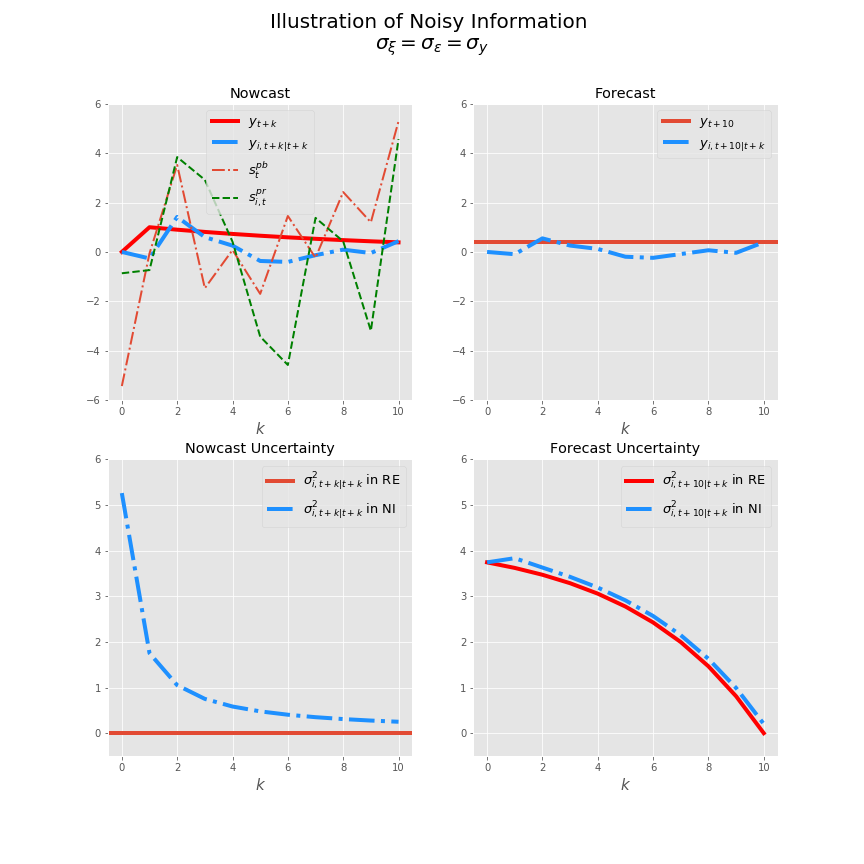
\includegraphics[height=0.8\textheight,width=\textwidth]{figuresDraft/ni_illustration} 
\end{figure}

\end{frame}



\begin{frame}{Impulse responses to shocks: individual moments}

$$\textrm{True Process} \quad   \rho=0.9, \quad \sigma_\omega= 1, \quad \omega_t = 1$$
$$ \textrm{SE:} \quad  \lambda = 0.25; \quad \textrm{NI:} \quad \sigma_\xi =  \sigma_\epsilon = \sigma_y$$

\begin{figure}
	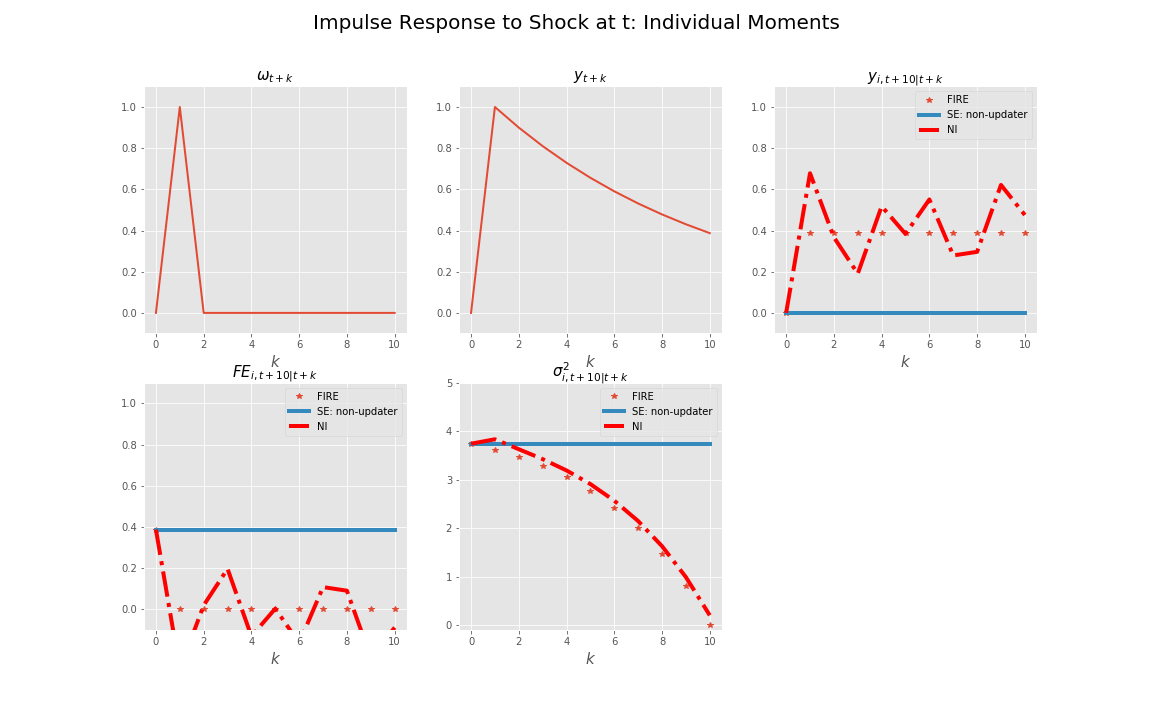
\includegraphics[height=0.6\textheight,width=\textwidth]{figuresDraft/ir_indseni} 
\end{figure}

\end{frame}

\begin{frame}{Impulse responses to shocks: population moments}

$$\textrm{True Process} \quad   \rho=0.9, \quad \sigma_\omega= 1, \quad \omega_t = 1$$
$$ \textrm{SE:} \quad  \lambda = 0.25; \quad \textrm{NI:} \quad \sigma_\xi =  \sigma_\epsilon = \sigma_y$$

\begin{figure}
	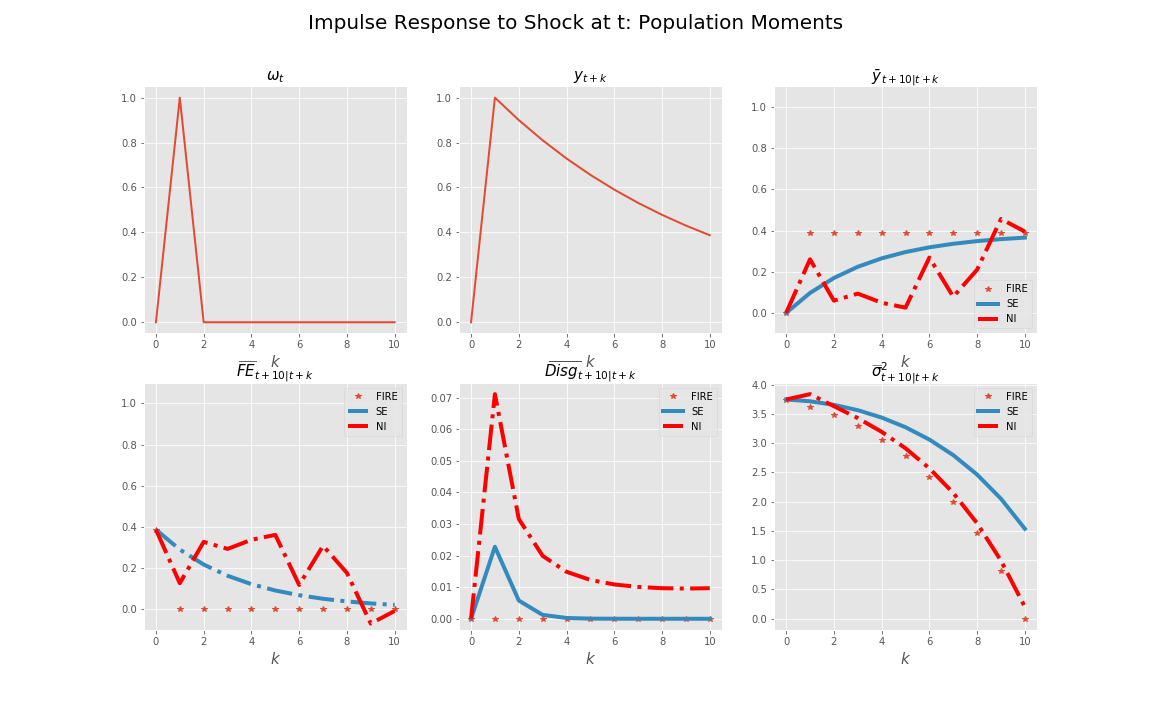
\includegraphics[height=0.6\textheight,width=\textwidth]{figuresDraft/ir_popseni} 
\end{figure}

\end{frame}

%\begin{frame}{Noisy Information: predictions}
%\begin{itemize}
%	\item \textbf{Similar to Sticky Expectation}
%	\begin{enumerate}
%\item \textbf{Macro rigidity}: population forecasts partially respond to shocks
% \item \textbf{Non-response of variance}: both individual and population variance \textcolor{blue}{does not respond to} shocks.   
% \end{enumerate}
%\item \textbf{Different from Sticky Expectation}

%	\begin{enumerate}
%	\item \textbf{Micro rigidity}: both individual and population forecast \textcolor{blue}{partially} respond to shocks 
%	\item \textbf{Horizon-sensitive rigidity}: rigidity decreases with horizon
%	\item \textbf{Increasing disagreements:} population disagreements \textcolor{blue}{increase} over time as approaching $t+h$
%	\item \textbf{Shock-specific responses:} different impacts of fundamental shocks, or simply news shocks 
%\end{enumerate}
%\end{itemize}

%\end{frame}



\begin{frame}{Comparing FIRE, SE and NI}


\begin{figure}
	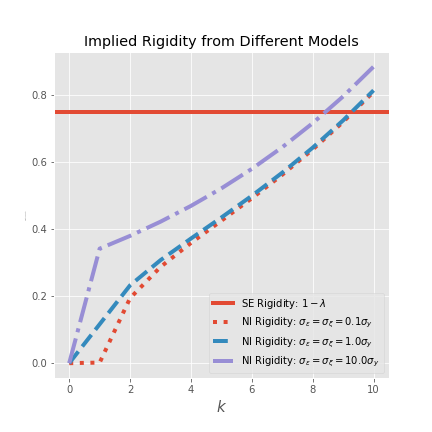
\includegraphics[height=5cm,width=8cm]{figuresDraft/rigidity} 
\end{figure}

\end{frame}



\begin{frame}{Other theories on to-do-list}
\begin{itemize}
	\item \textbf{Rational Inattention:} attentiveness endogenously respond to variances
	\item \textbf{Learning}: the structural parameter $\rho$ is not known, thus the agent learns about it as if an econometrician does
\end{itemize}
\end{frame}

\begin{frame}{Identification strategies 1: testing rigidity models}

\begin{itemize}
	\item \citet{coibion2012can}
	\begin{itemize}
		\item \textcolor{blue}{FEs} respond to shocks and serially correlated. 
	\end{itemize}
	\item \textbf{Additional in this paper}
	\begin{itemize}
		\item \textcolor{blue}{Uncertainty} does not depend on shocks; and serially correlated. 
	\end{itemize}
\end{itemize}

\end{frame}

\begin{frame}{Identification strategies 2: differentiating theories}
\begin{itemize}
	\item \citet{coibion2012can}
	\begin{itemize}
		\item \textcolor{blue}{FEs} do not depend on past realizations according to baseline SE and NI; but do so according to heterogeneous priors or precision models. 
		\item Implied rigidity does not differ across shocks according to SE but differs according to NI. 
		\item \textcolor{blue}{Disagreements} rise after shocks according to baseline SE, strategic interactions and heterogeneous priors but invariant according to baseline NI.
	\end{itemize}
	\item \textbf{Additional in this paper}
	\begin{itemize}
		\item \textcolor{blue}{Uncertainty} do not depend on shocks per se according to baseline SE and NI, instead on degree of information rigidity.
	\end{itemize}
\end{itemize}

\end{frame}

\section{Data and Methodology}


\begin{frame}{Data}
\begin{table}[]
\resizebox{\textwidth}{!}{	\begin{tabular}{lll}
		
		\hline 
		& SCE & SPF        \\
		\hline 
		Time period                                    & 2013-present                            & 2007-present             \\
		Frequency                                      & Monthly                                 & Quarterly                \\
		Sample Size                                    & 1,300                                   & 30-50                    \\
		Aggregate Var in Density                       & \textcolor{blue}{1-yr and 3-yr inflation}          & \textcolor{blue}{1-yr and 3-yr CPI and PCE}         \\
		Pannel Structure                               & stay up to 12 months                    & average stay for 5 years \\
		Demographic Info                        & Education, Income, Age        & Industry    \\
		\hline 
	\end{tabular}}
\end{table}

\end{frame}



\section{Stylized Facts}

\begin{frame}{Uncertainty and Realized Inflation}
\begin{figure}
	\centering
\label{InfVar}
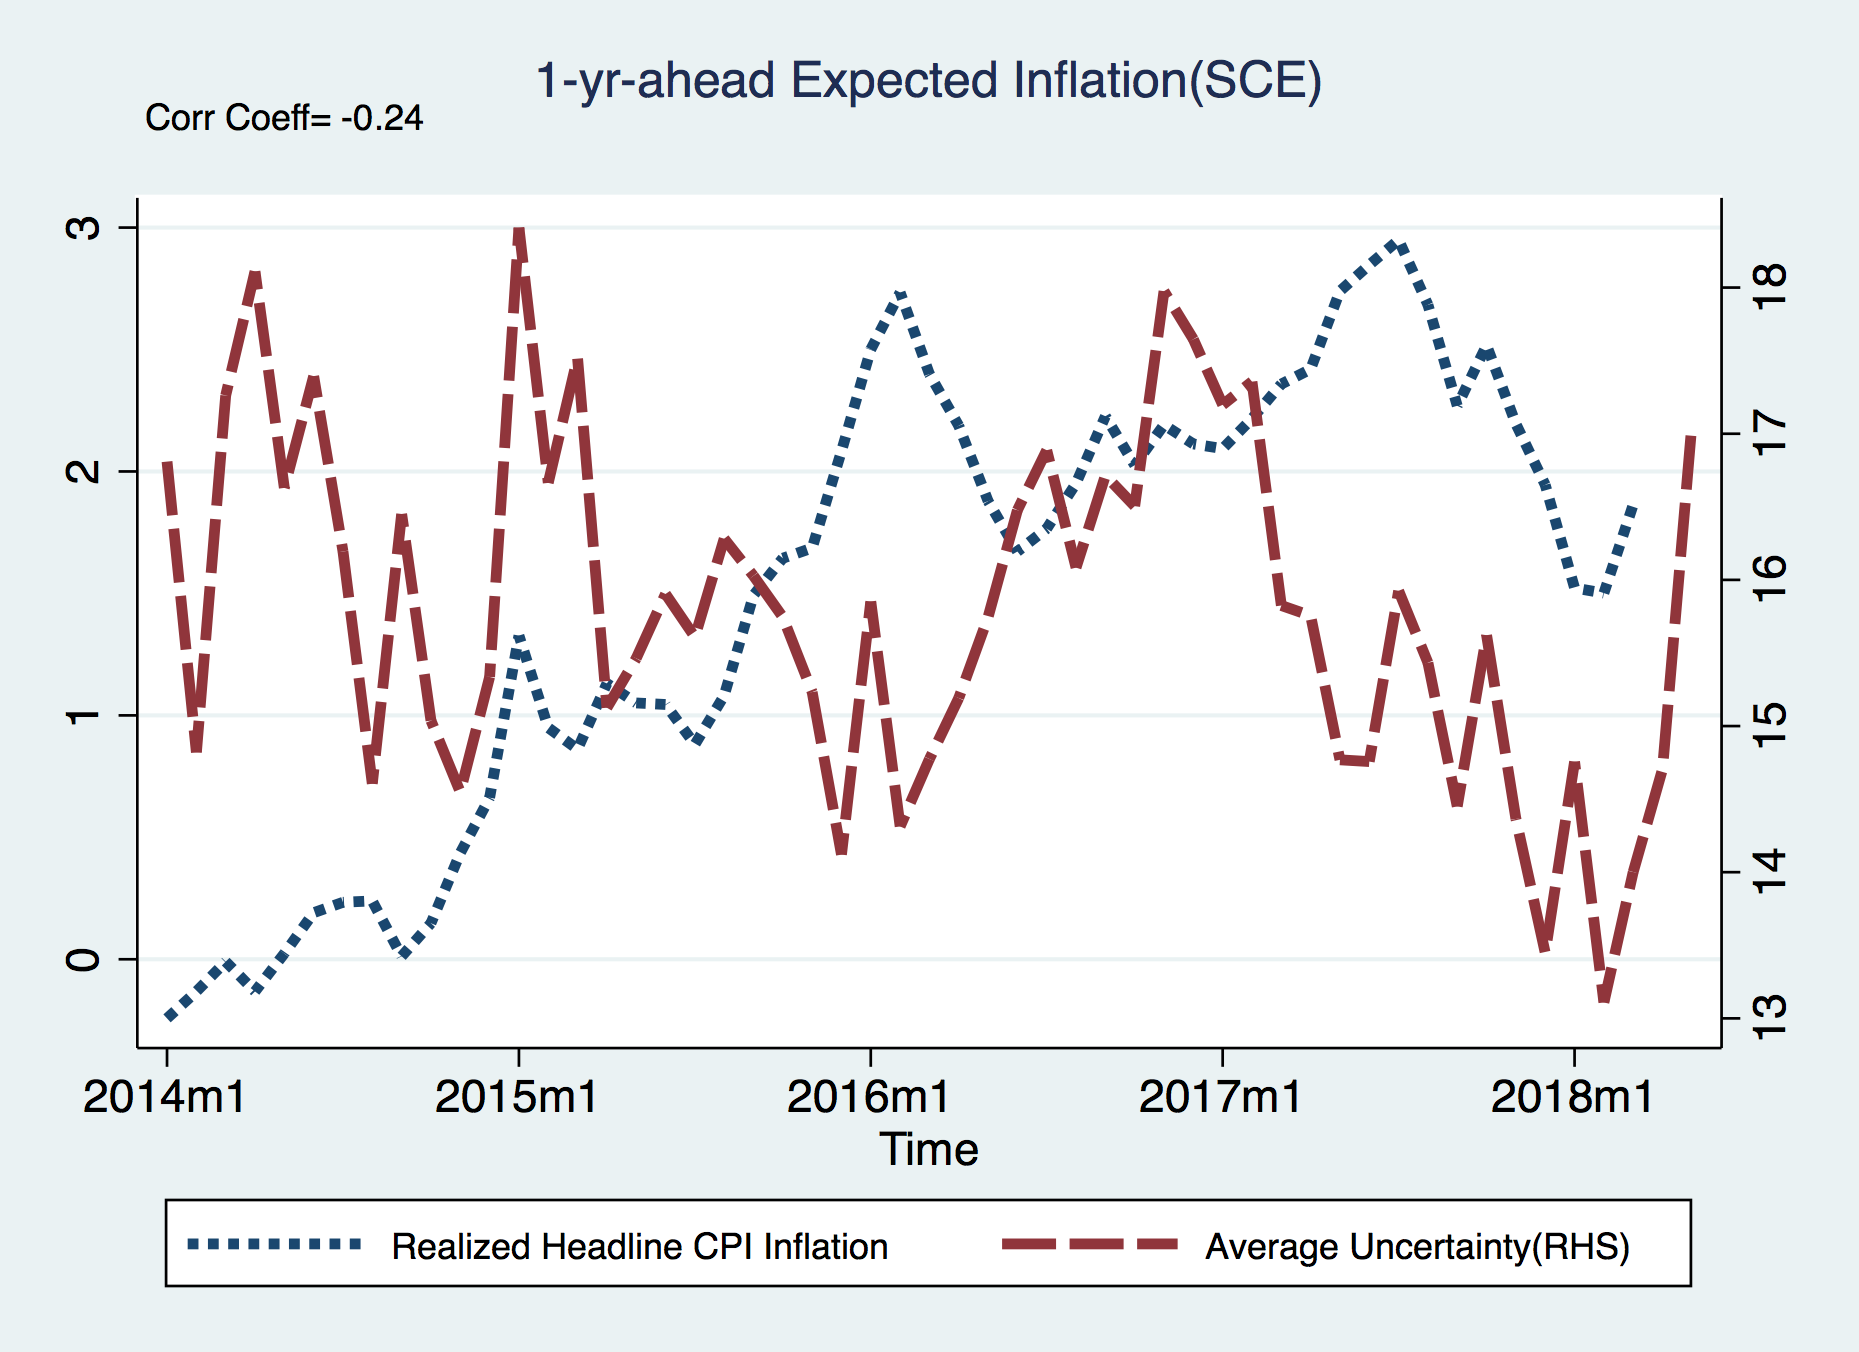
\includegraphics[width=0.33\textwidth]{figuresDraft/Inf1yf_CPIAU_varSCEM.png}
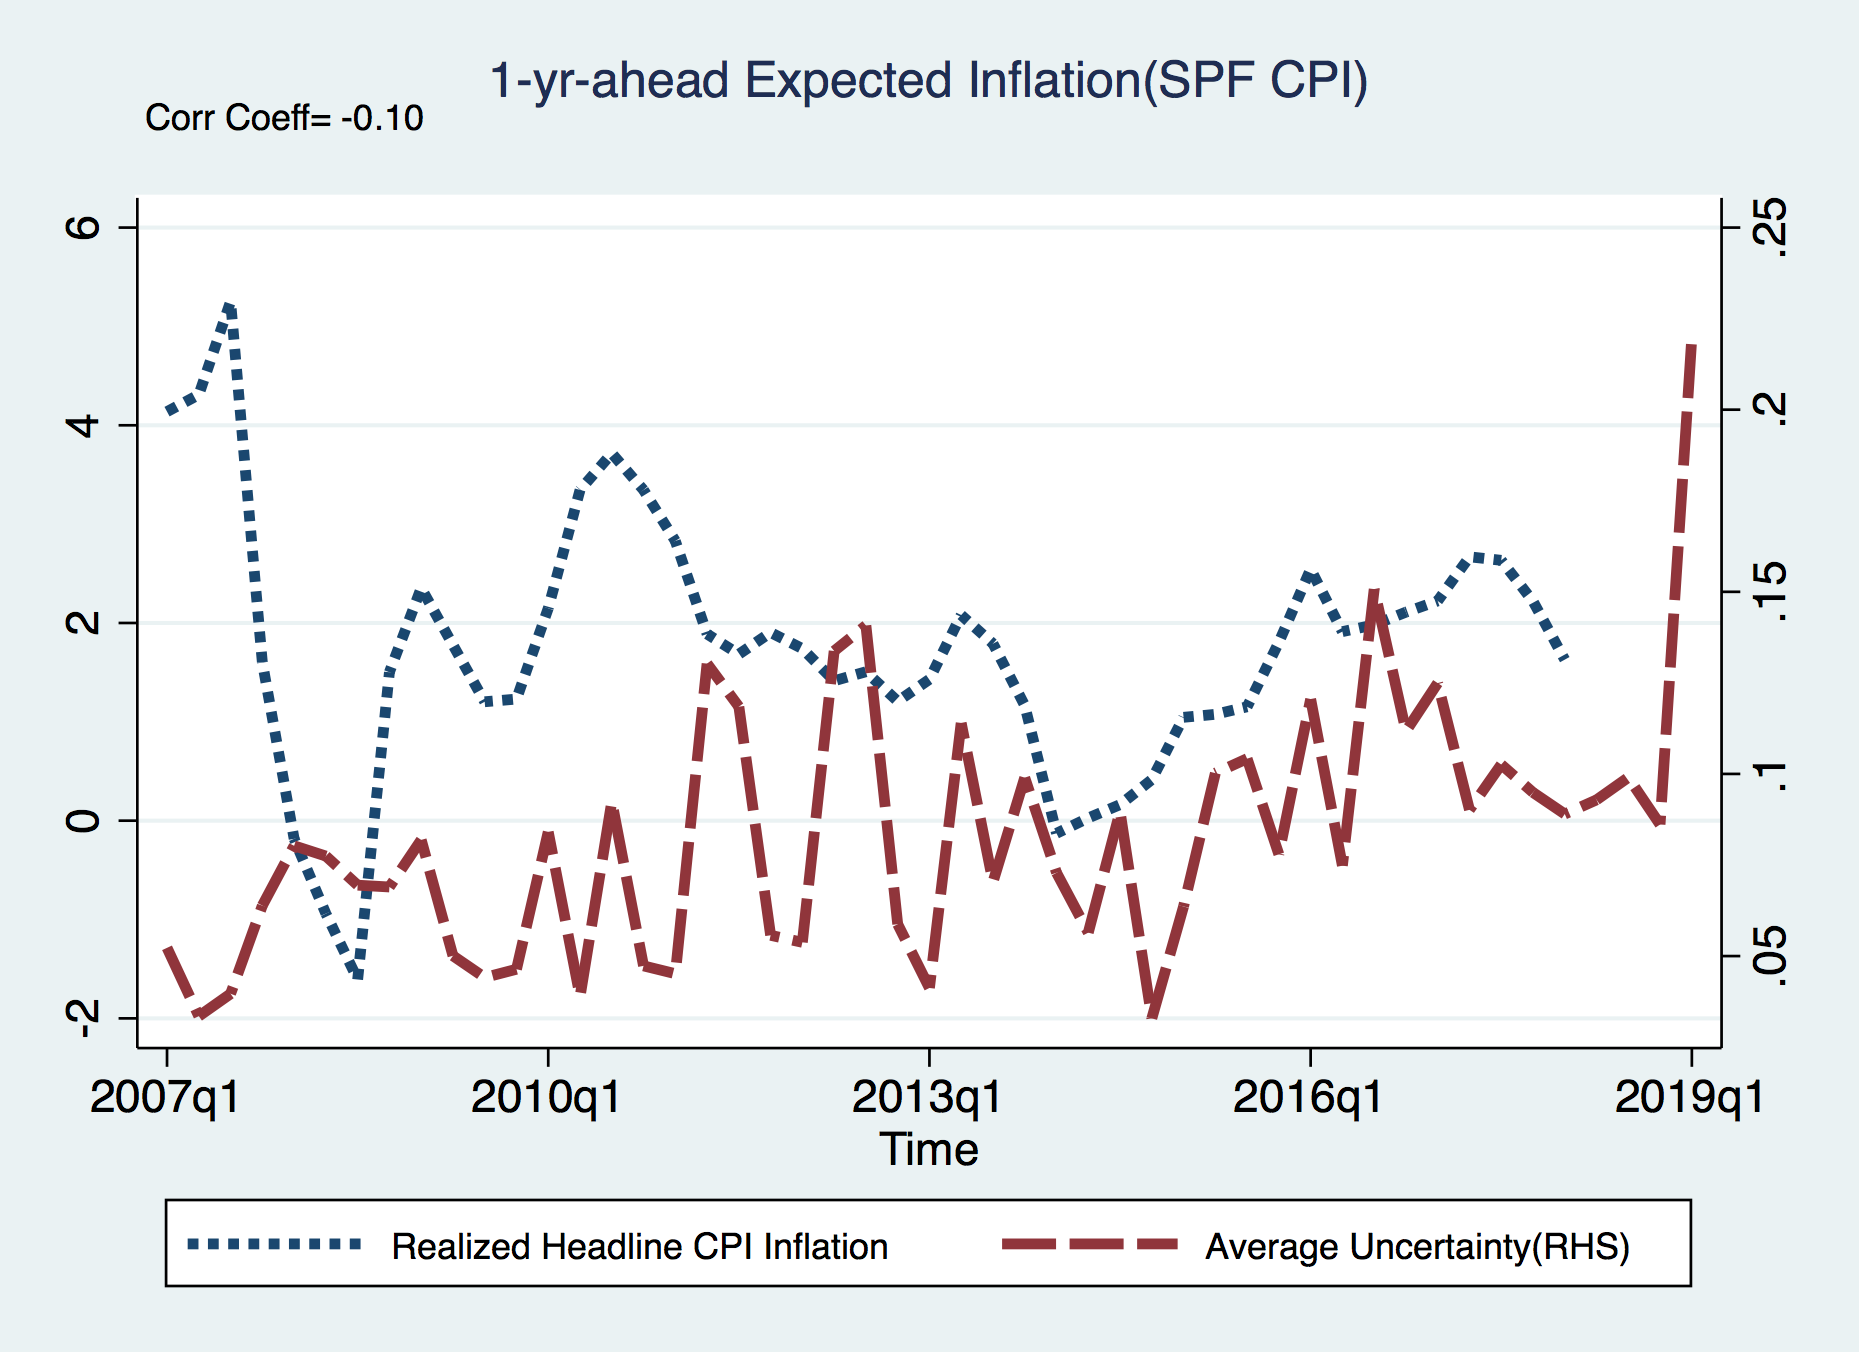
\includegraphics[width=0.33\textwidth]{figuresDraft/Inf1yf_CPIAU_varSPFCPIQ.png}
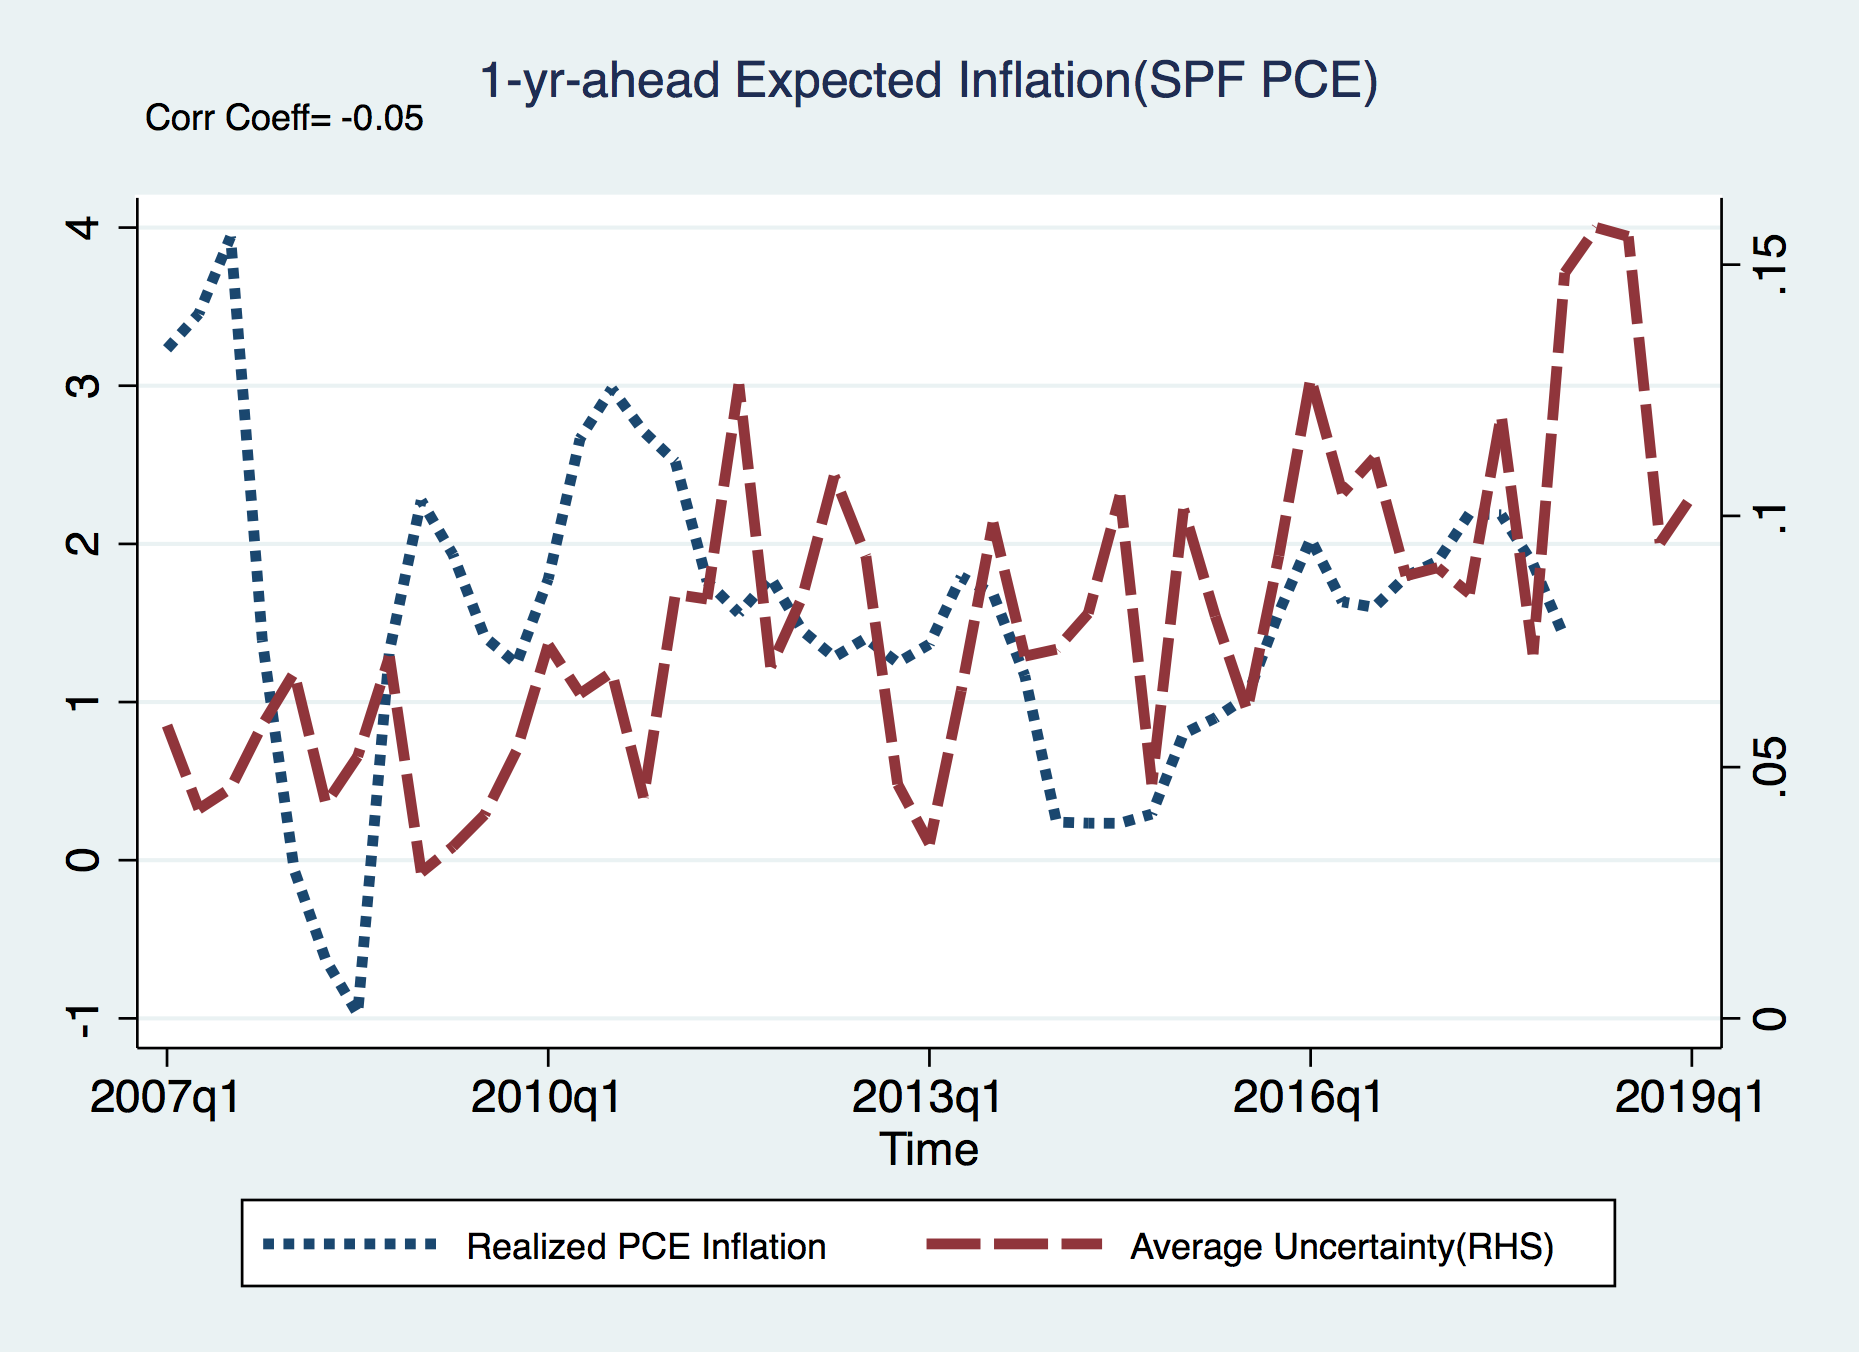
\includegraphics[width=0.33\textwidth]{figuresDraft/Inf1yf_PCE_varSPFPCEQ.png}
\end{figure}
\end{frame}

\begin{frame}{Uncertainty and Forecast Errors}
\begin{figure}
	\centering
	\label{FEVar}
	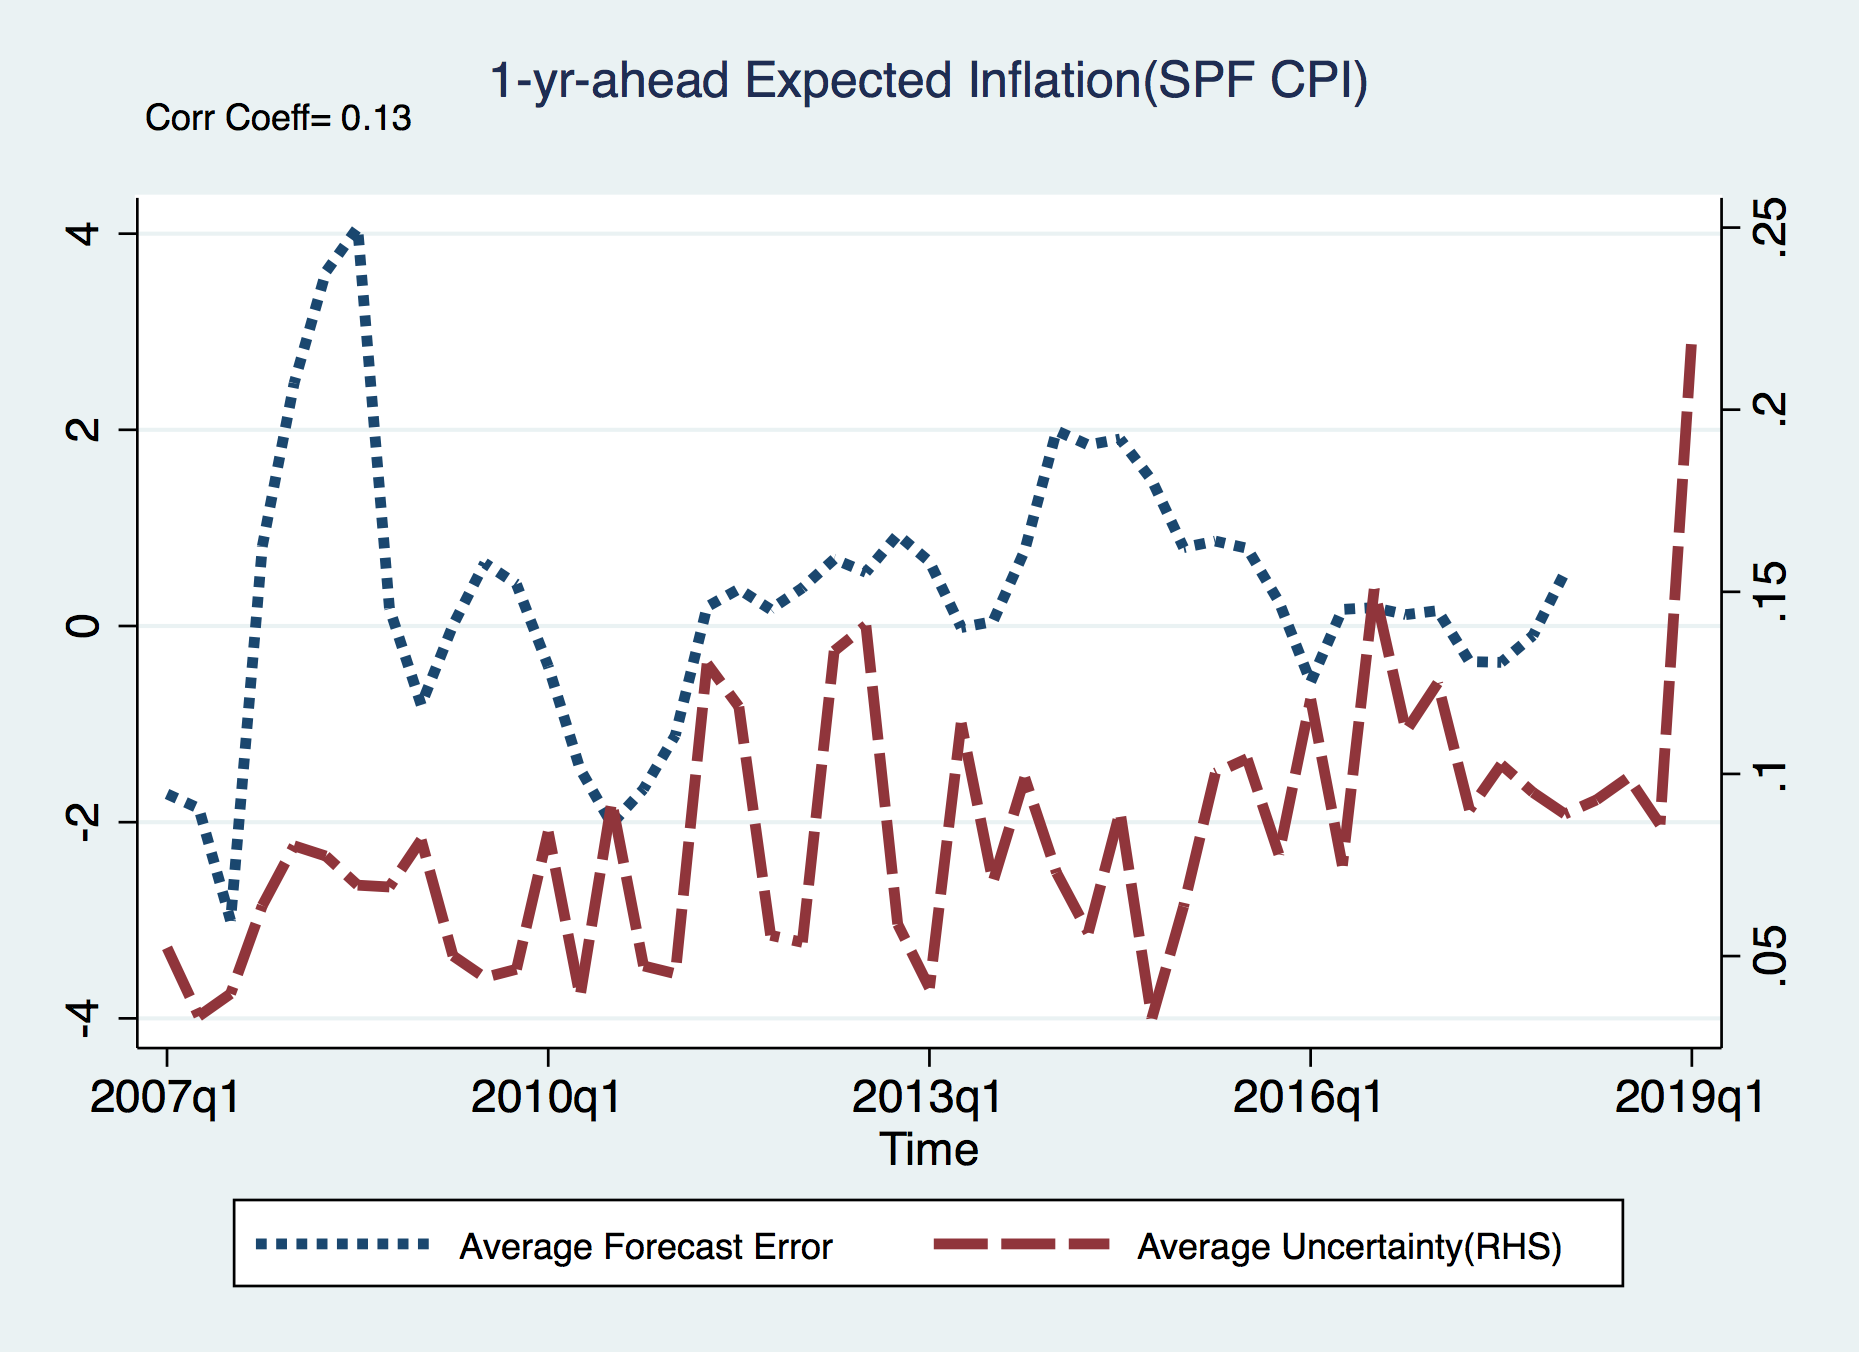
\includegraphics[width=0.33\textwidth]{figuresDraft/SPFCPI_FE_varSPFCPIQ.png}
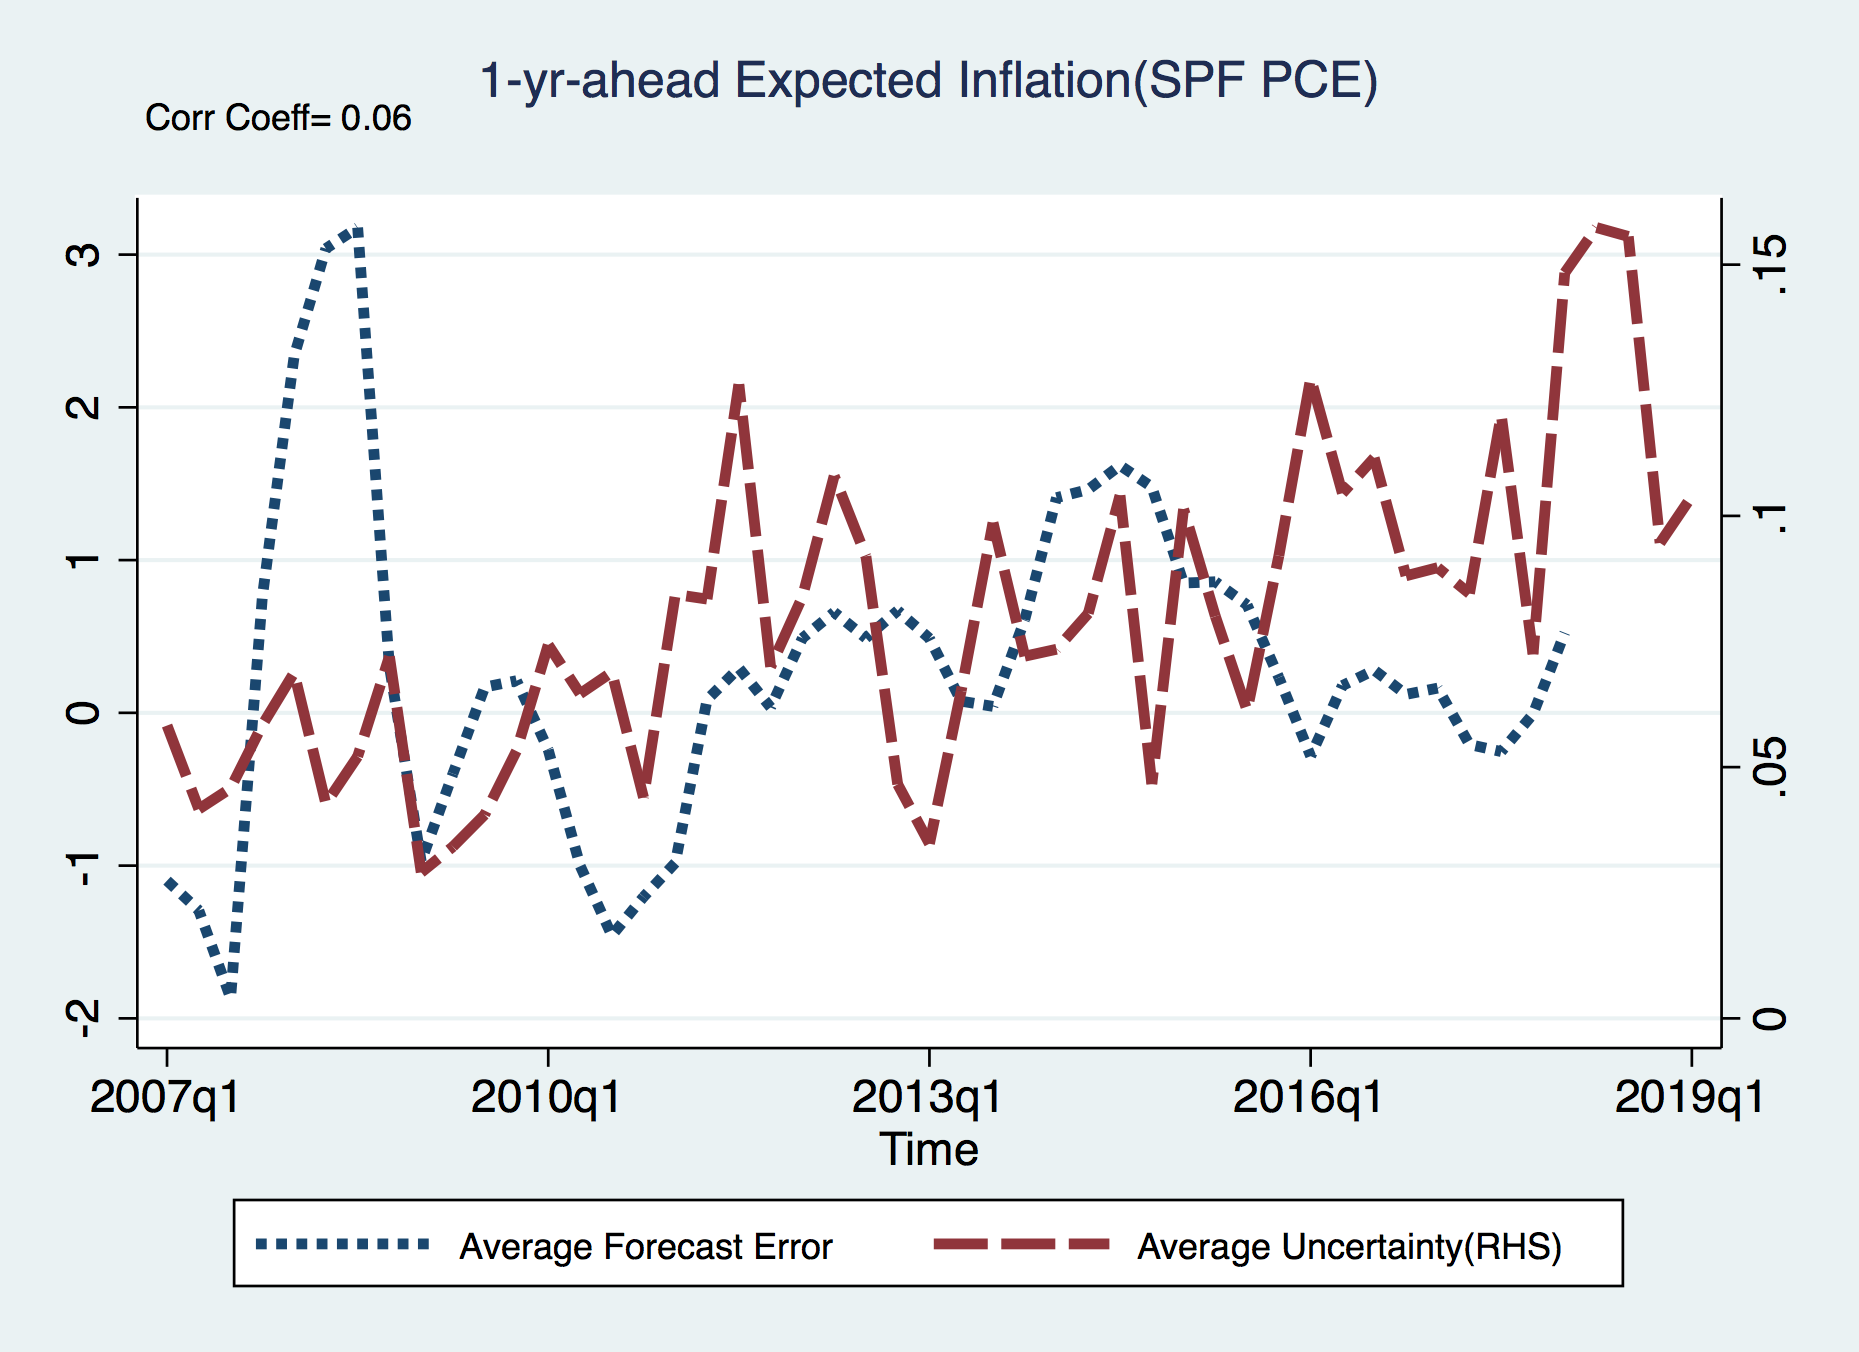
\includegraphics[width=0.33\textwidth]{figuresDraft/SPFPCE_FE_varSPFPCEQ.png}
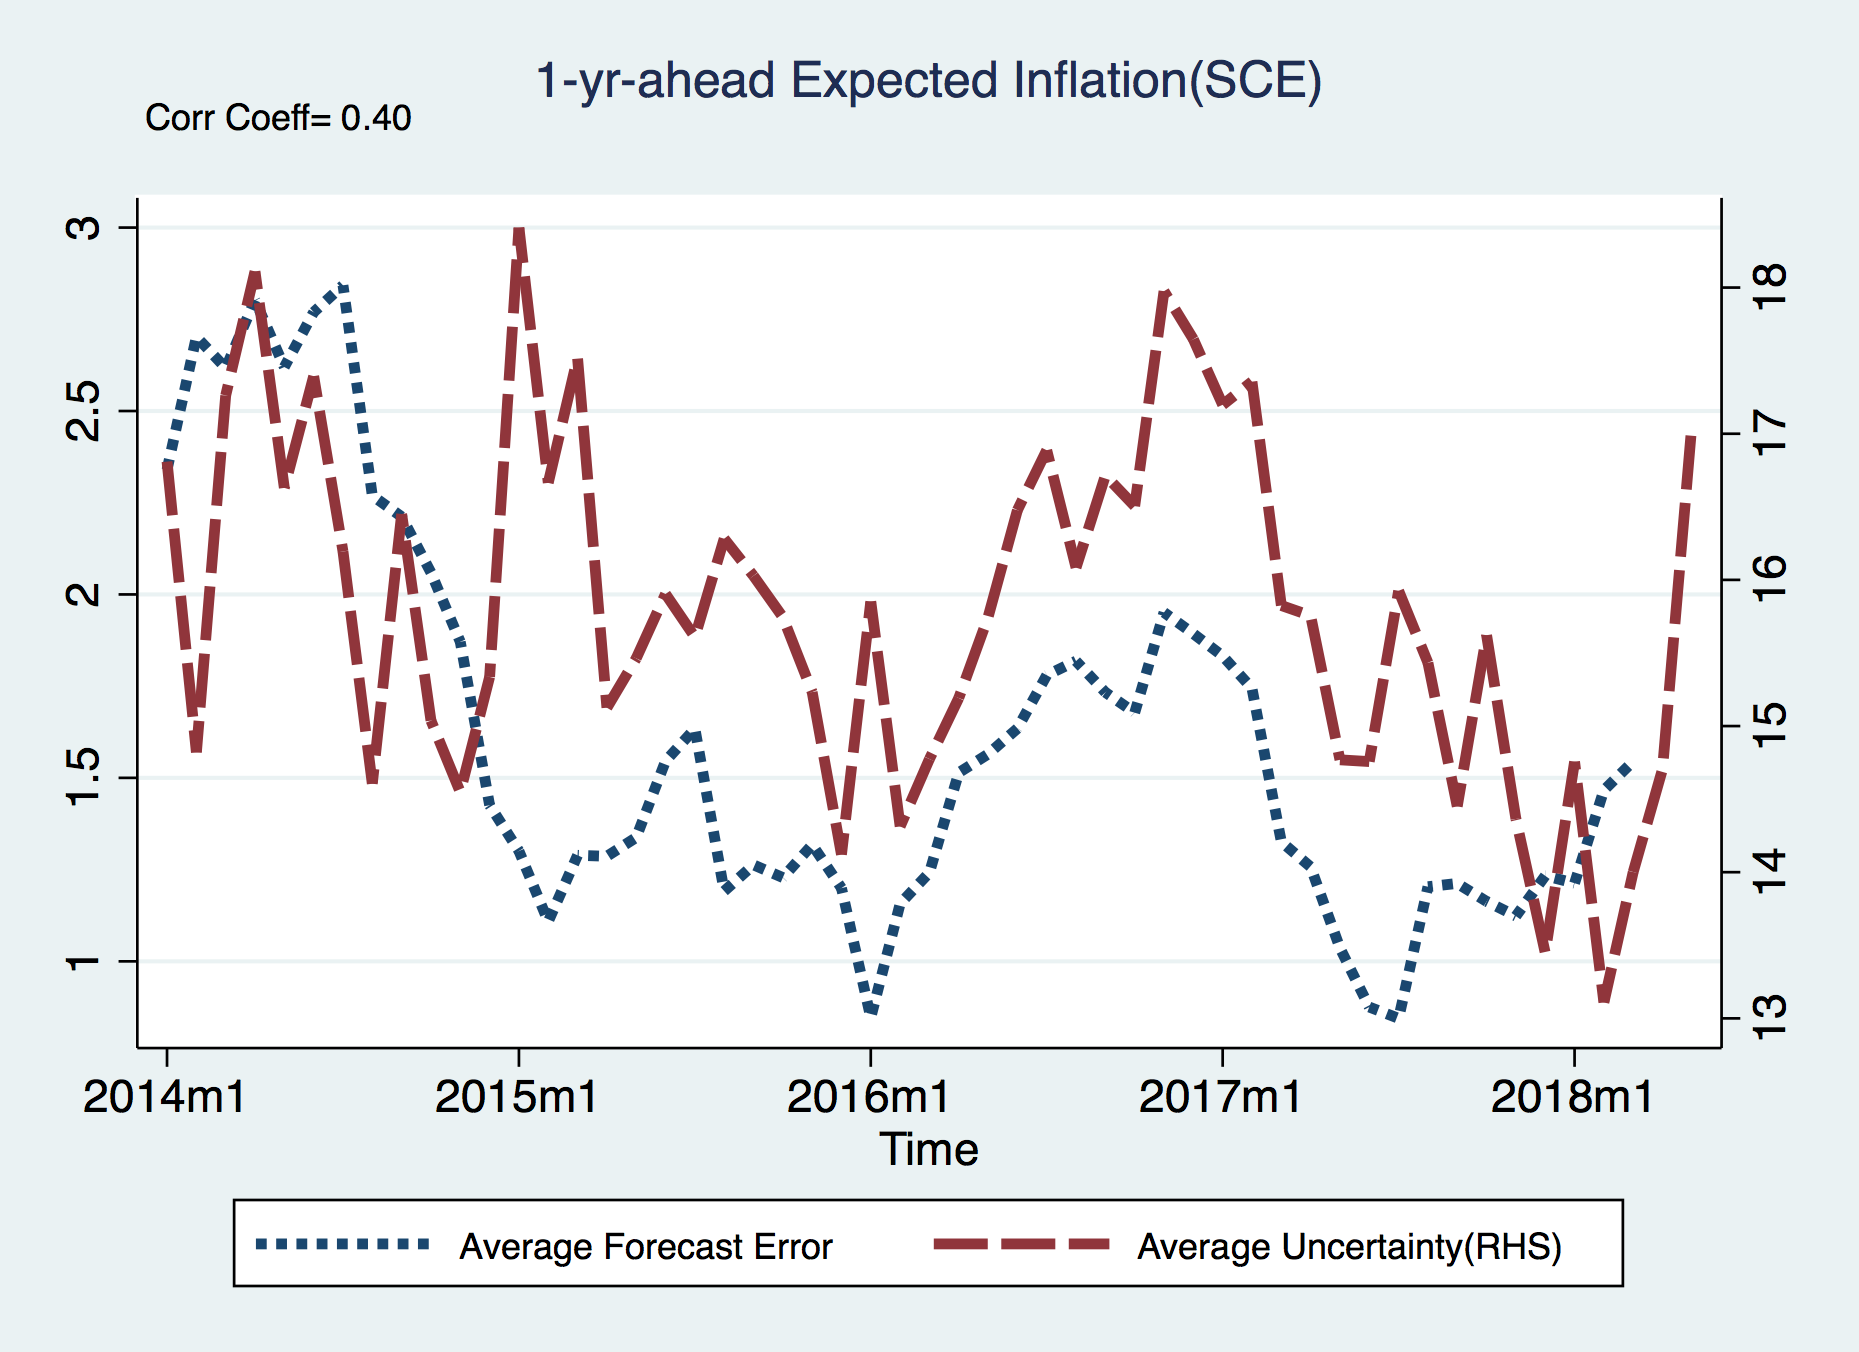
\includegraphics[width=0.33\textwidth]{figuresDraft/SCE_FE_varSCEM.png}
\end{figure}
\end{frame}


\begin{frame}{Uncertainty and Disagreements}
\begin{figure}
	\centering
\label{DisgVar}
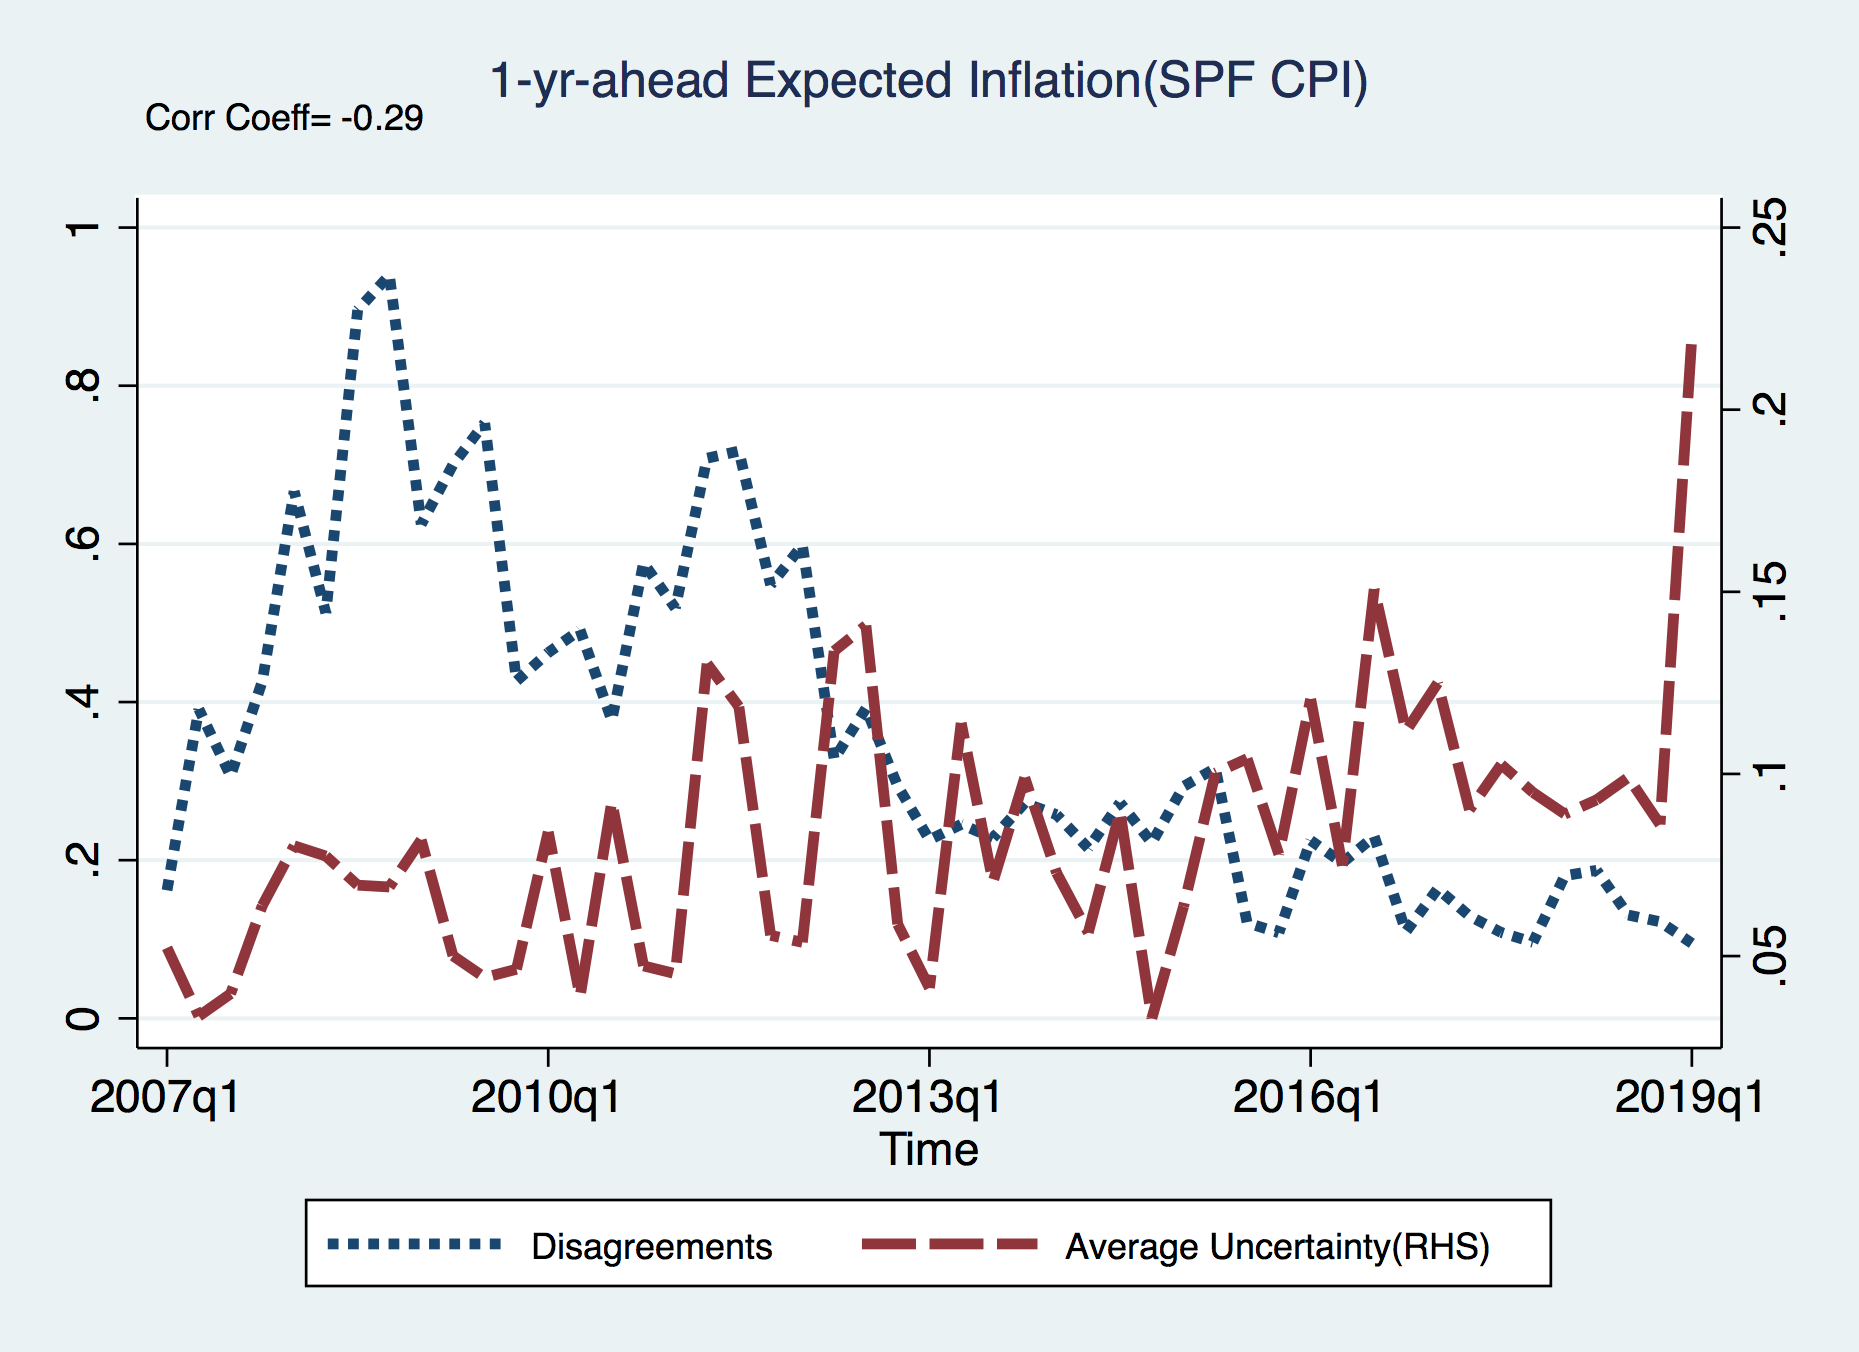
\includegraphics[width=0.33\textwidth]{figuresDraft/CPI_disg_varSPFCPIQ.png}
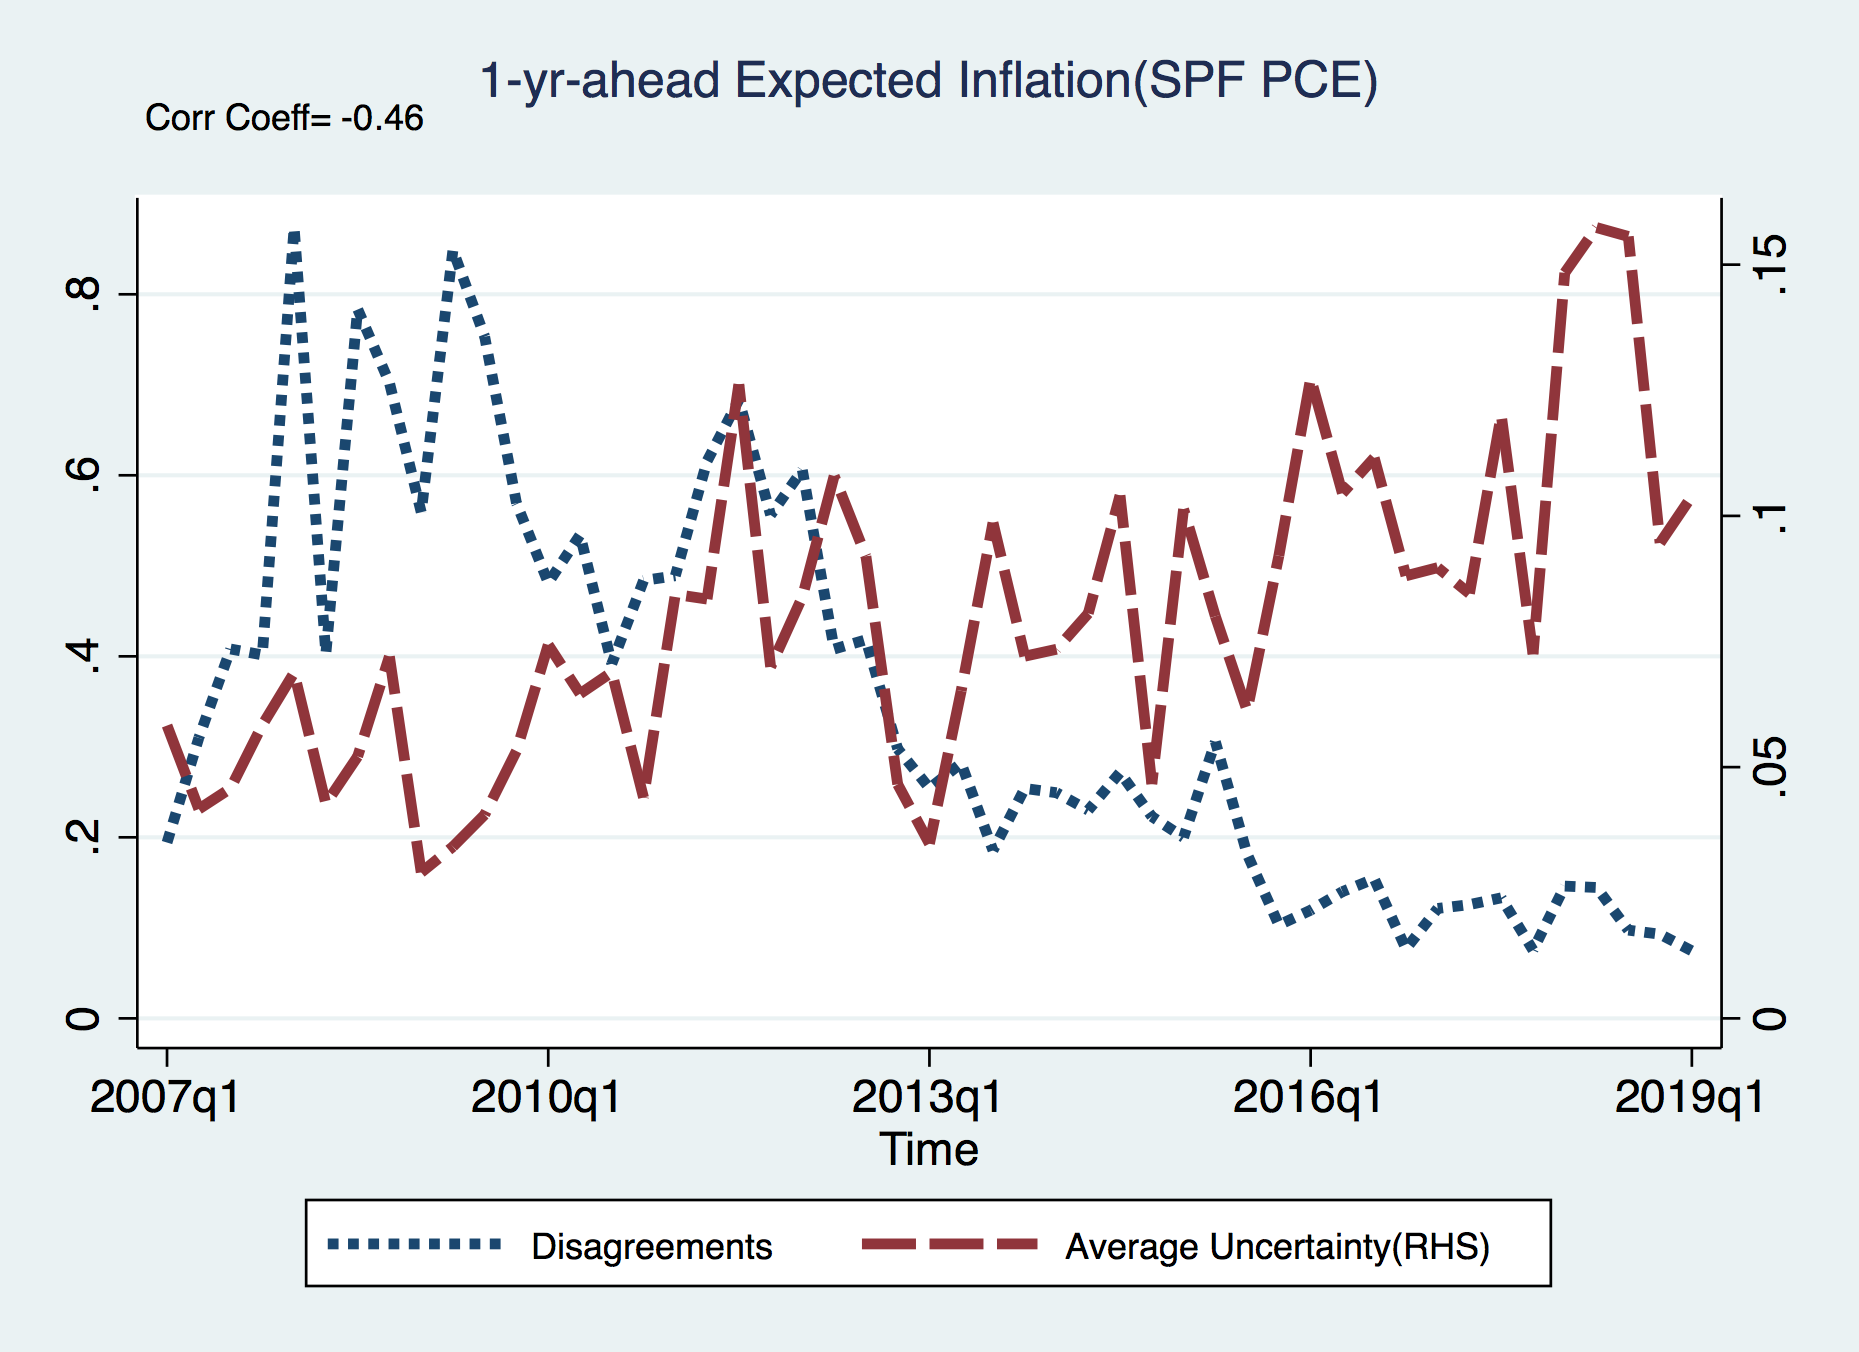
\includegraphics[width=0.33\textwidth]{figuresDraft/PCE_disg_varSPFPCEQ.png}
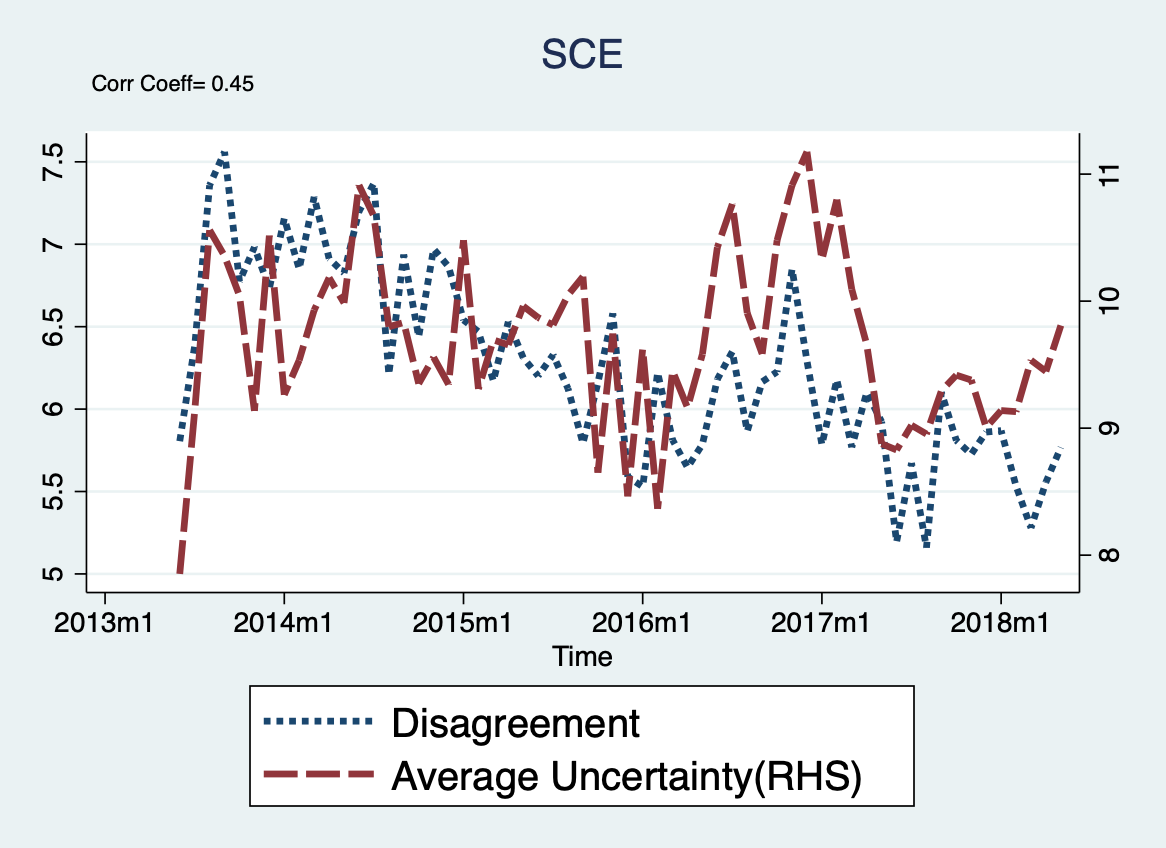
\includegraphics[width=0.33\textwidth]{figuresDraft/Q9_disg_varSCEM.png}
\end{figure}
\end{frame}



\begin{frame}{Dispersion of Mean Forecast}
\begin{figure}
	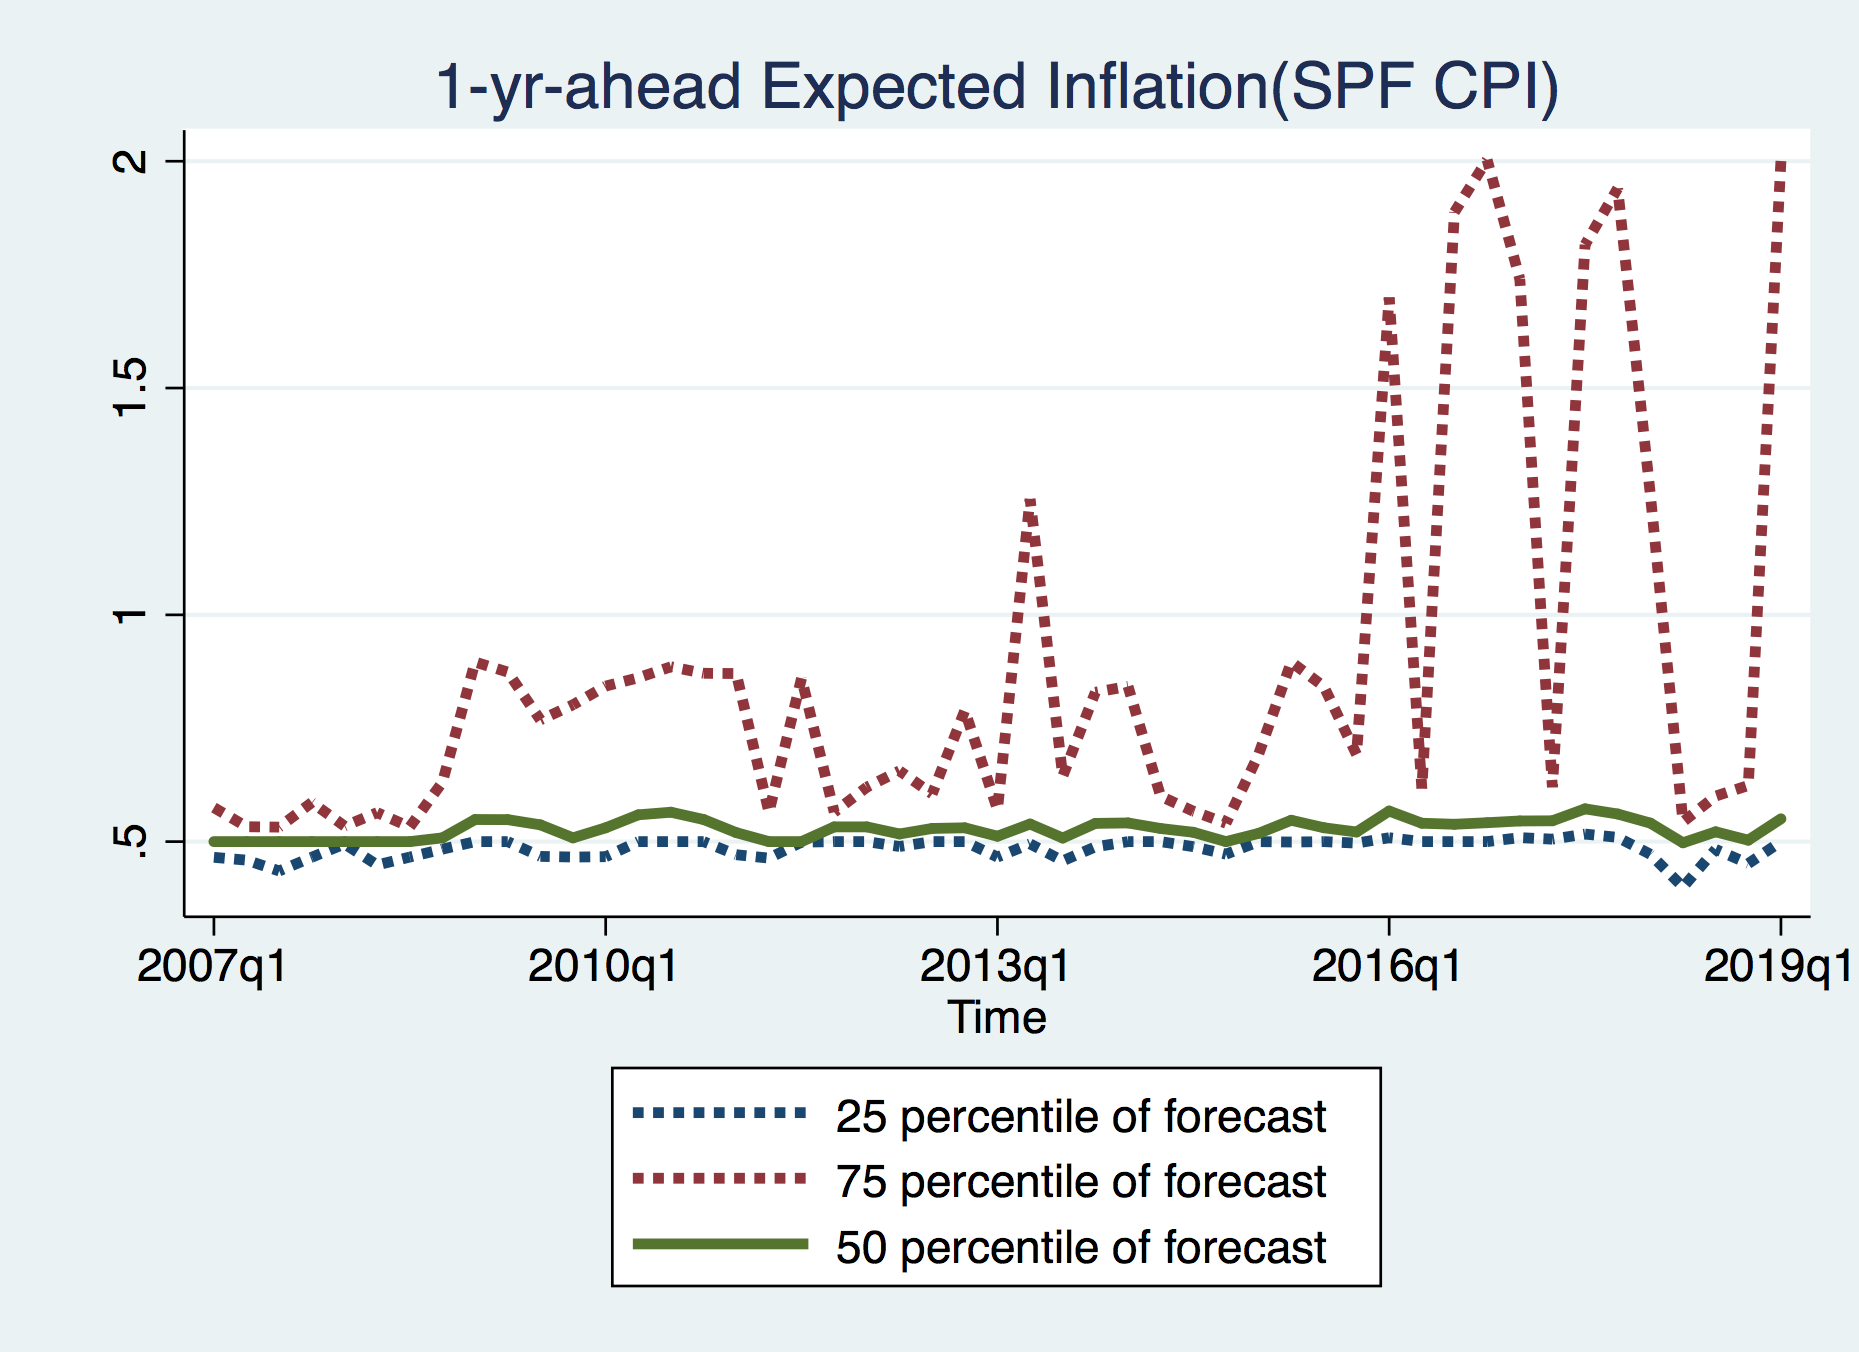
\includegraphics[width=0.33\textwidth]{figuresDraft/IQRmeanCPIQ.png} 
\smallskip
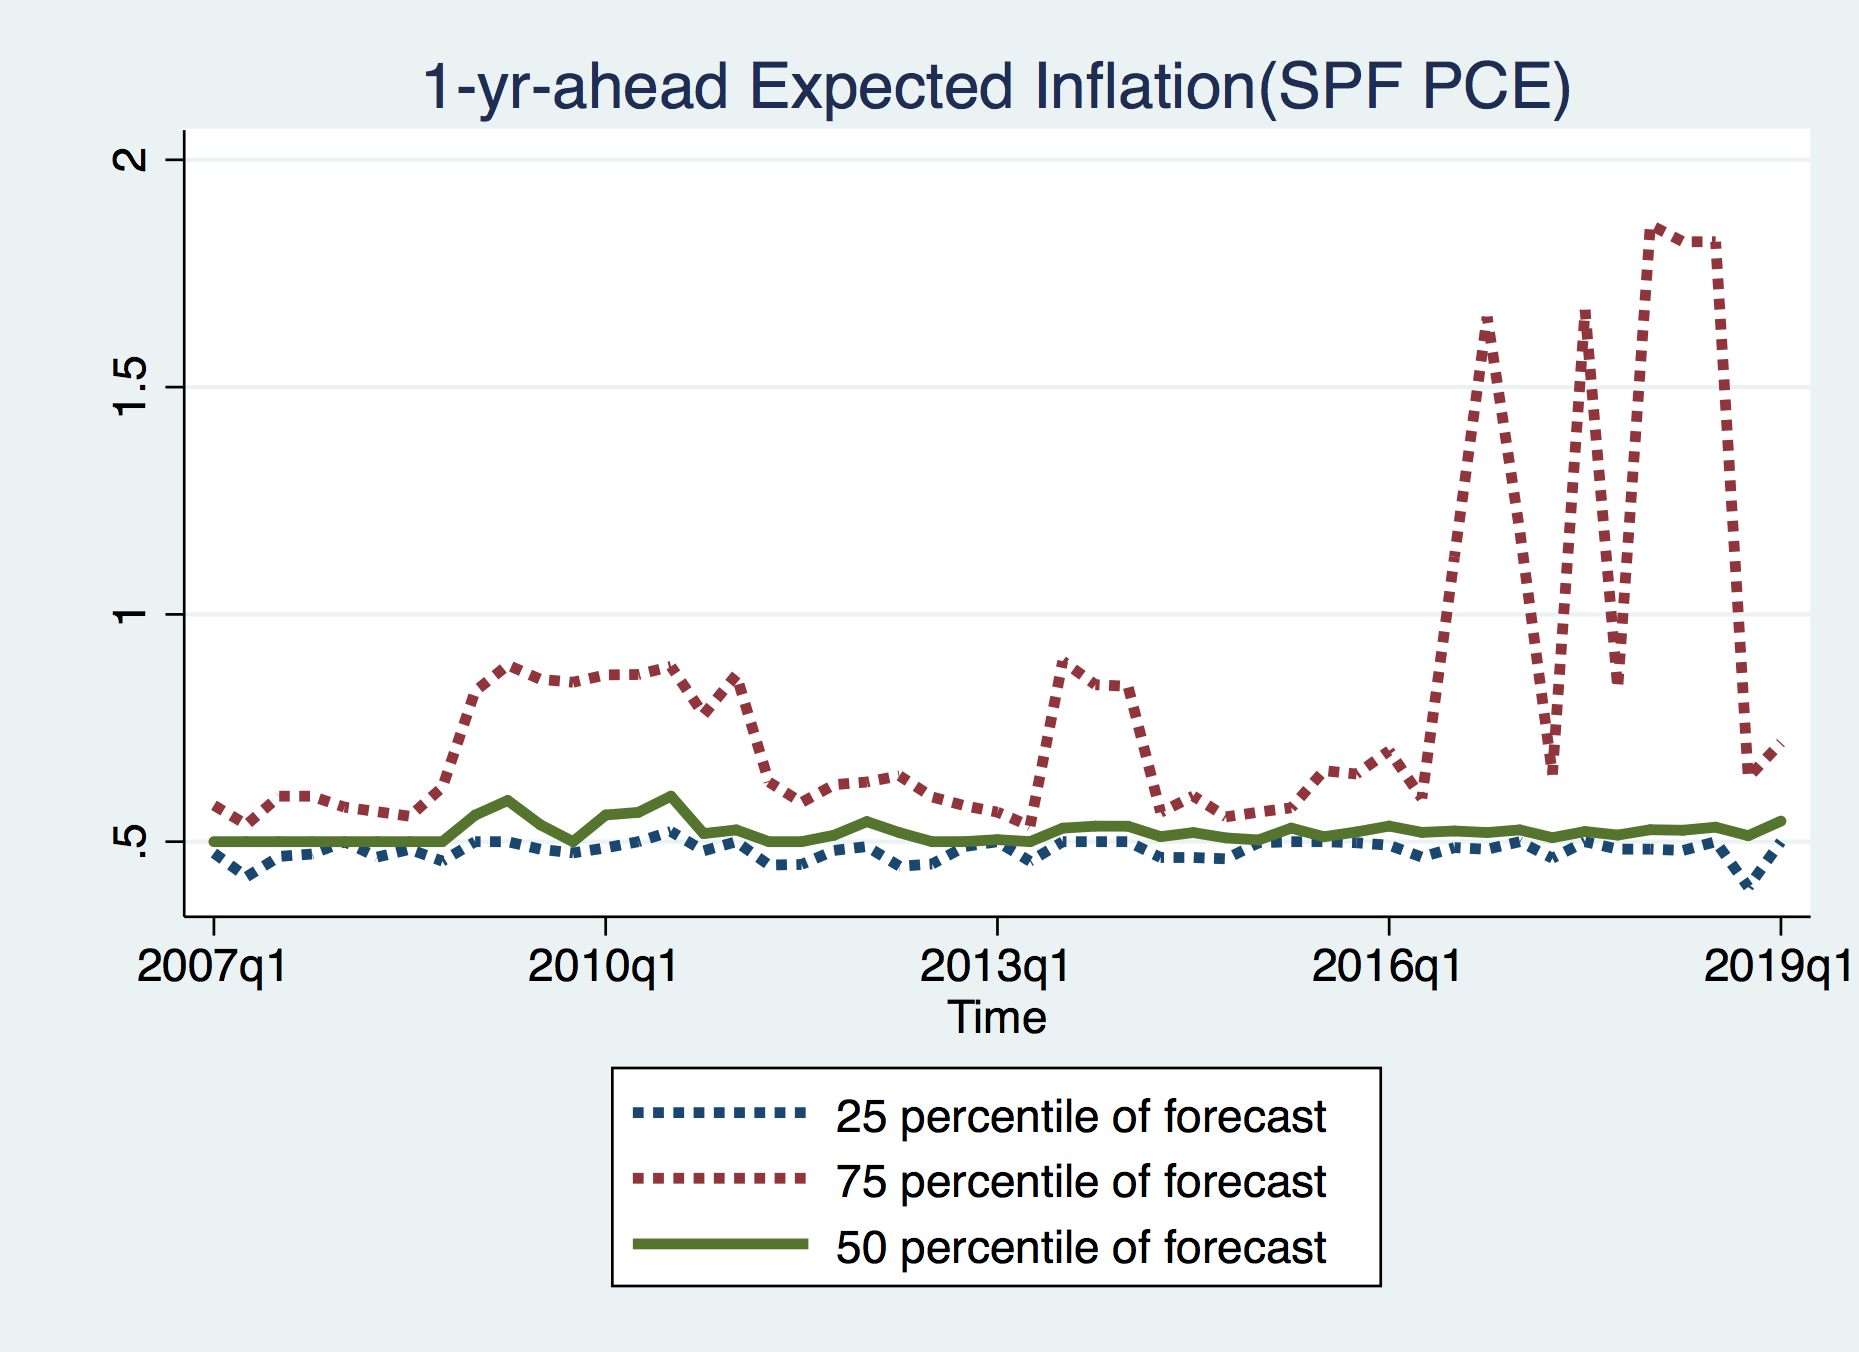
\includegraphics[width=0.33\textwidth]{figuresDraft/IQRmeanPCEQ.png}
\smallskip
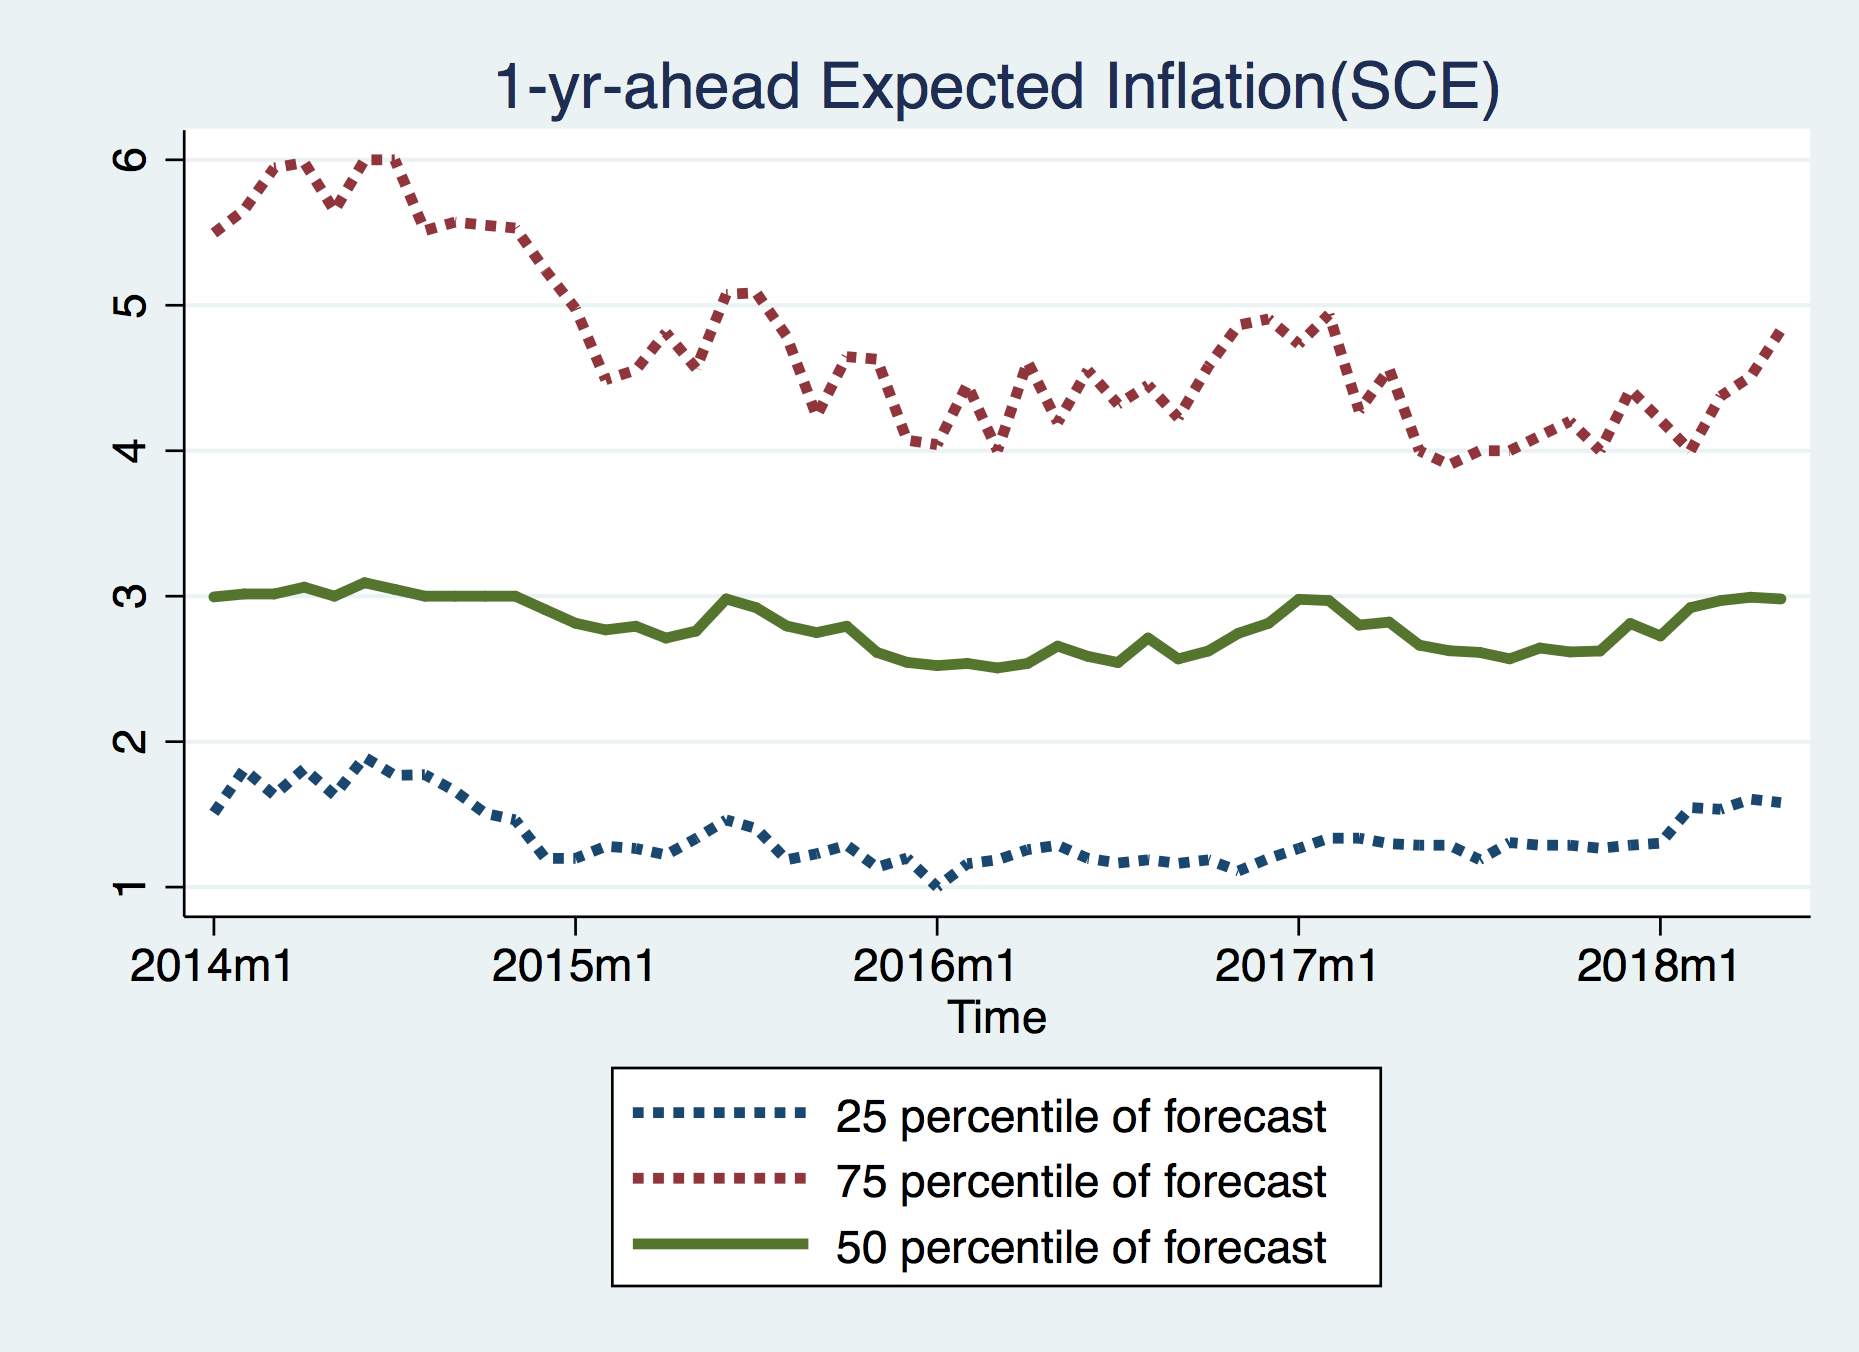
\includegraphics[width=0.33\textwidth]{figuresDraft/IQRmeanSCEM.png}
\end{figure}
\end{frame}


\begin{frame}{Dispersion of Uncertainty}
\begin{figure}
	\label{IQR_Unceratitny}
	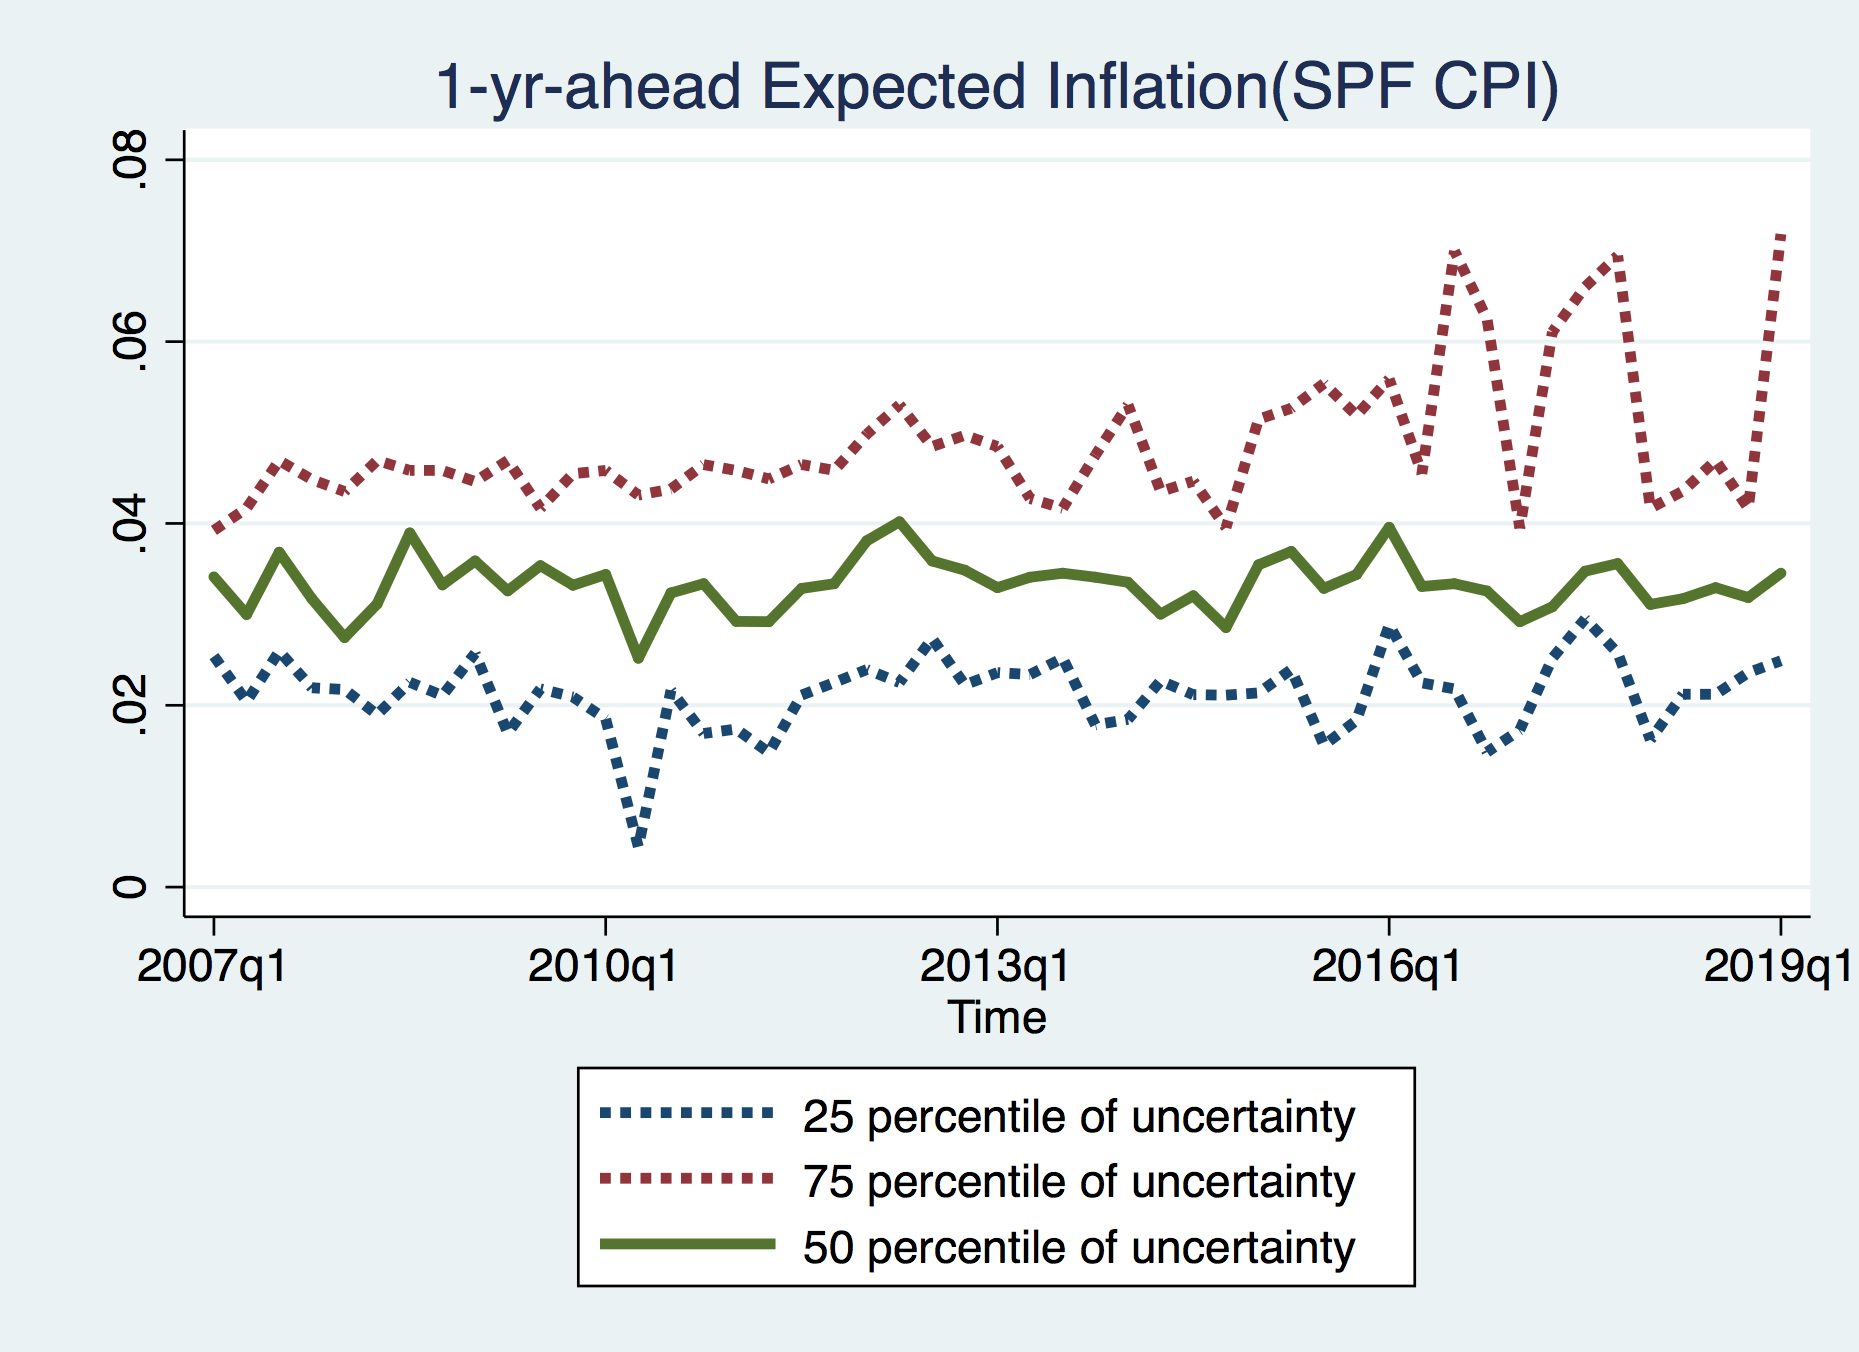
\includegraphics[width=0.33\textwidth]{figuresDraft/IQRvarCPIQ.png}
\smallskip
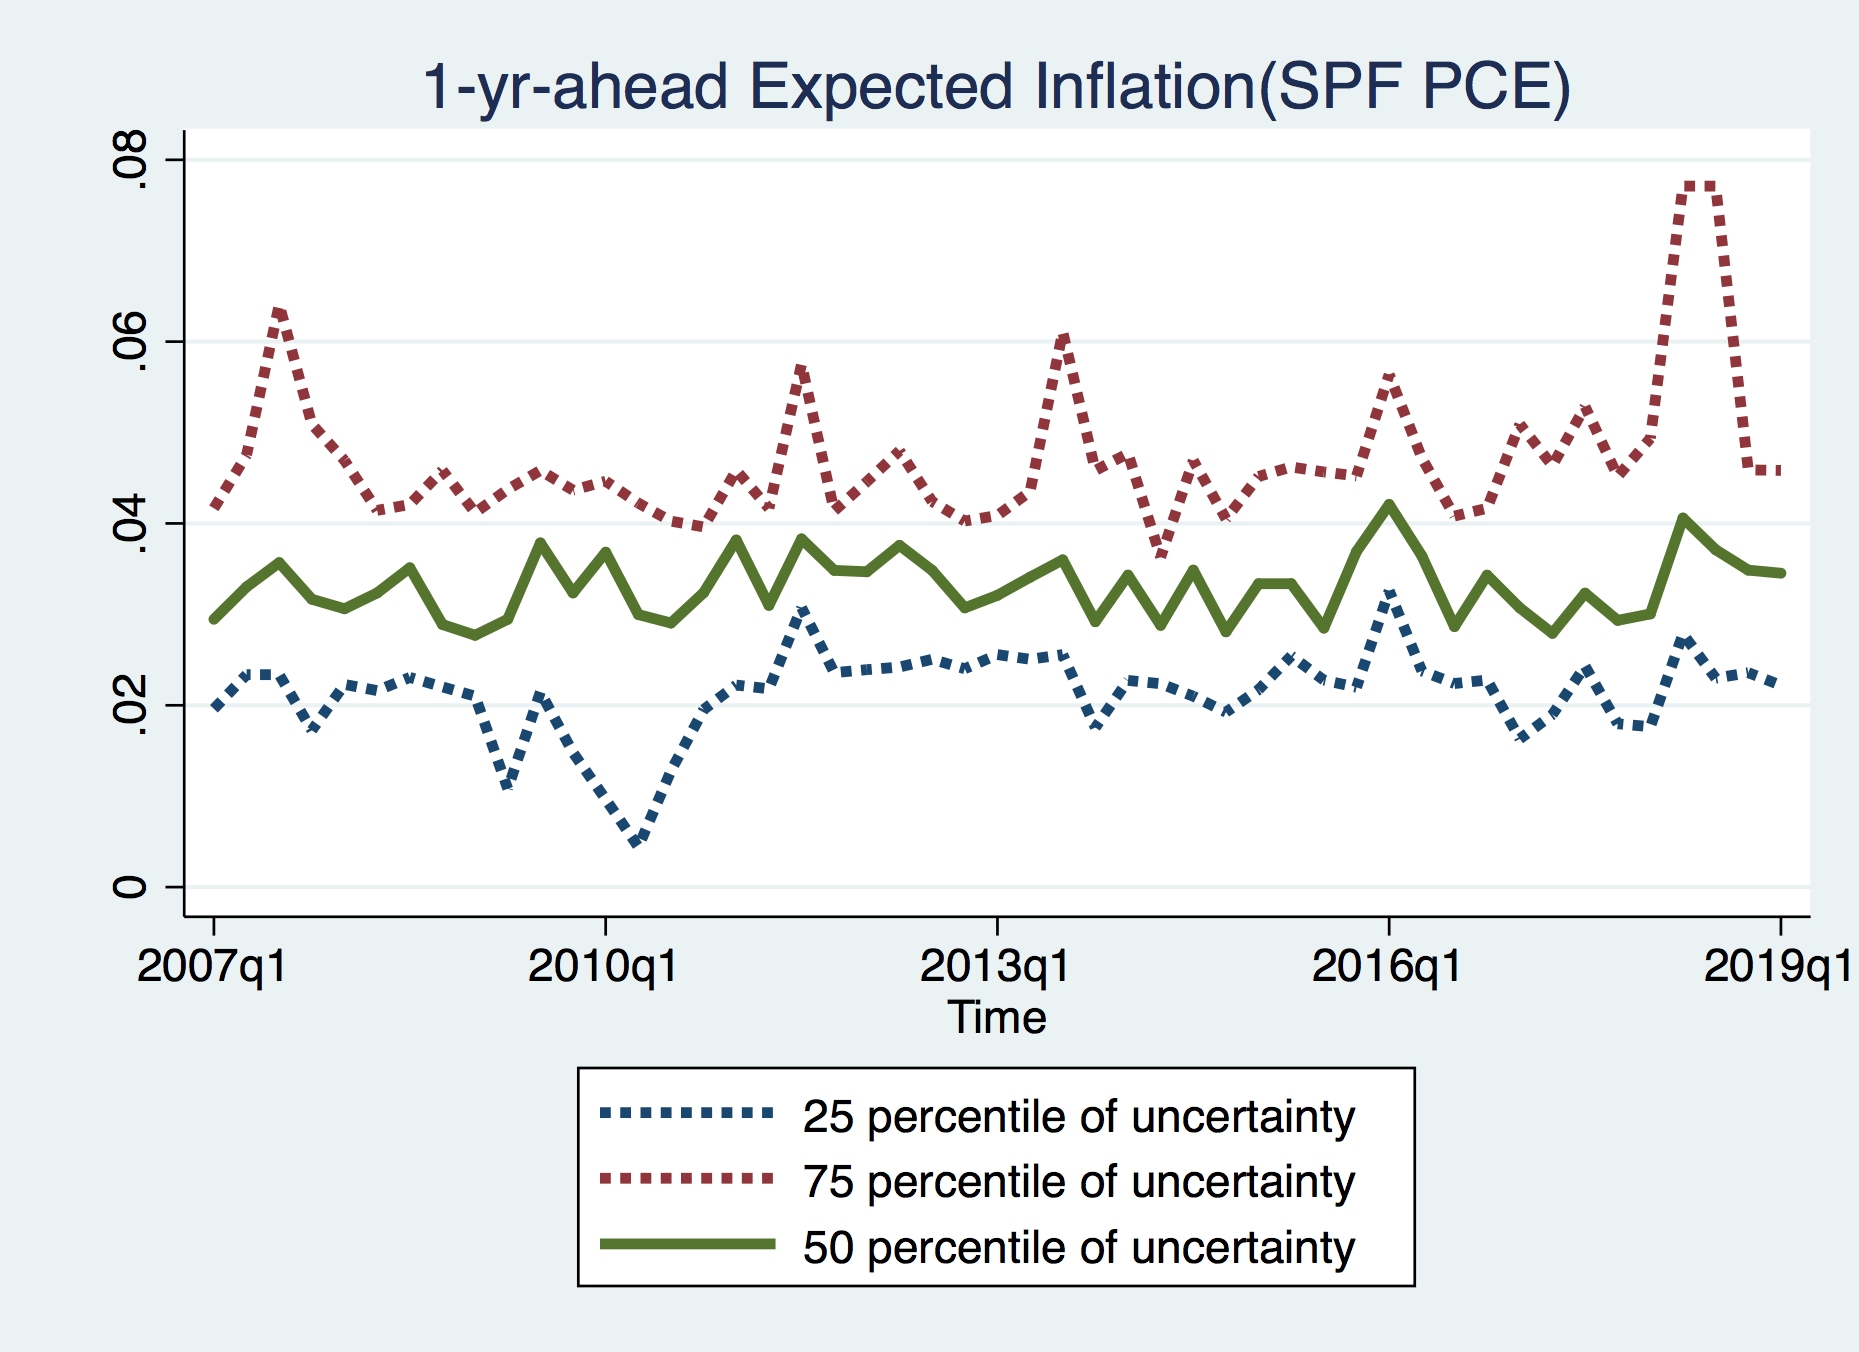
\includegraphics[width=0.33\textwidth]{figuresDraft/IQRvarPCEQ.png}
\smallskip
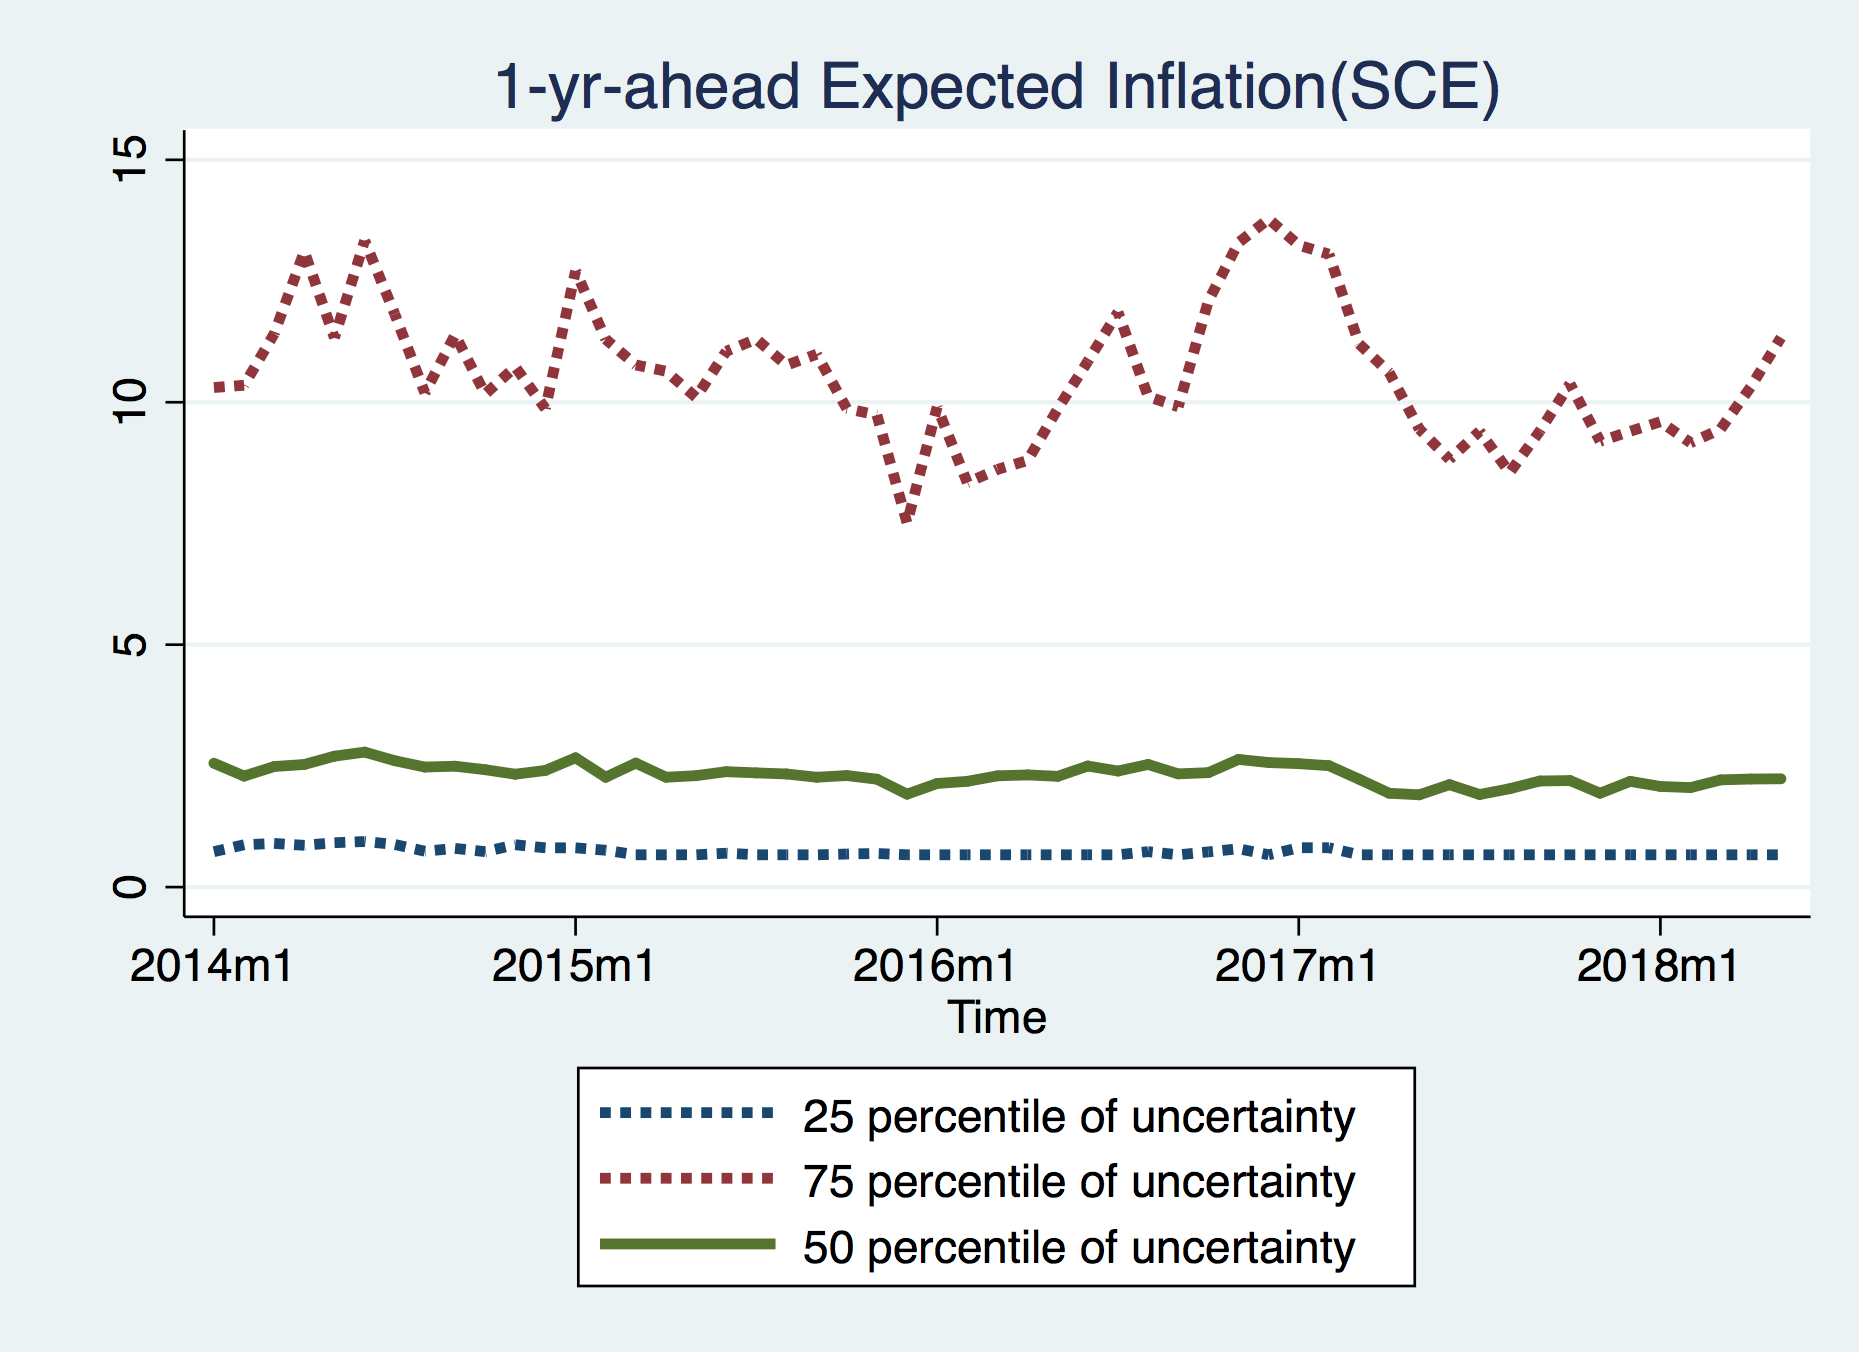
\includegraphics[width=0.33\textwidth]{figuresDraft/IQRvarSCEM.png}
\end{figure}
\end{frame}


\begin{frame}{Distribution of Uncertainty}
\begin{figure}
		\label{Unceratitny_Histogram}
	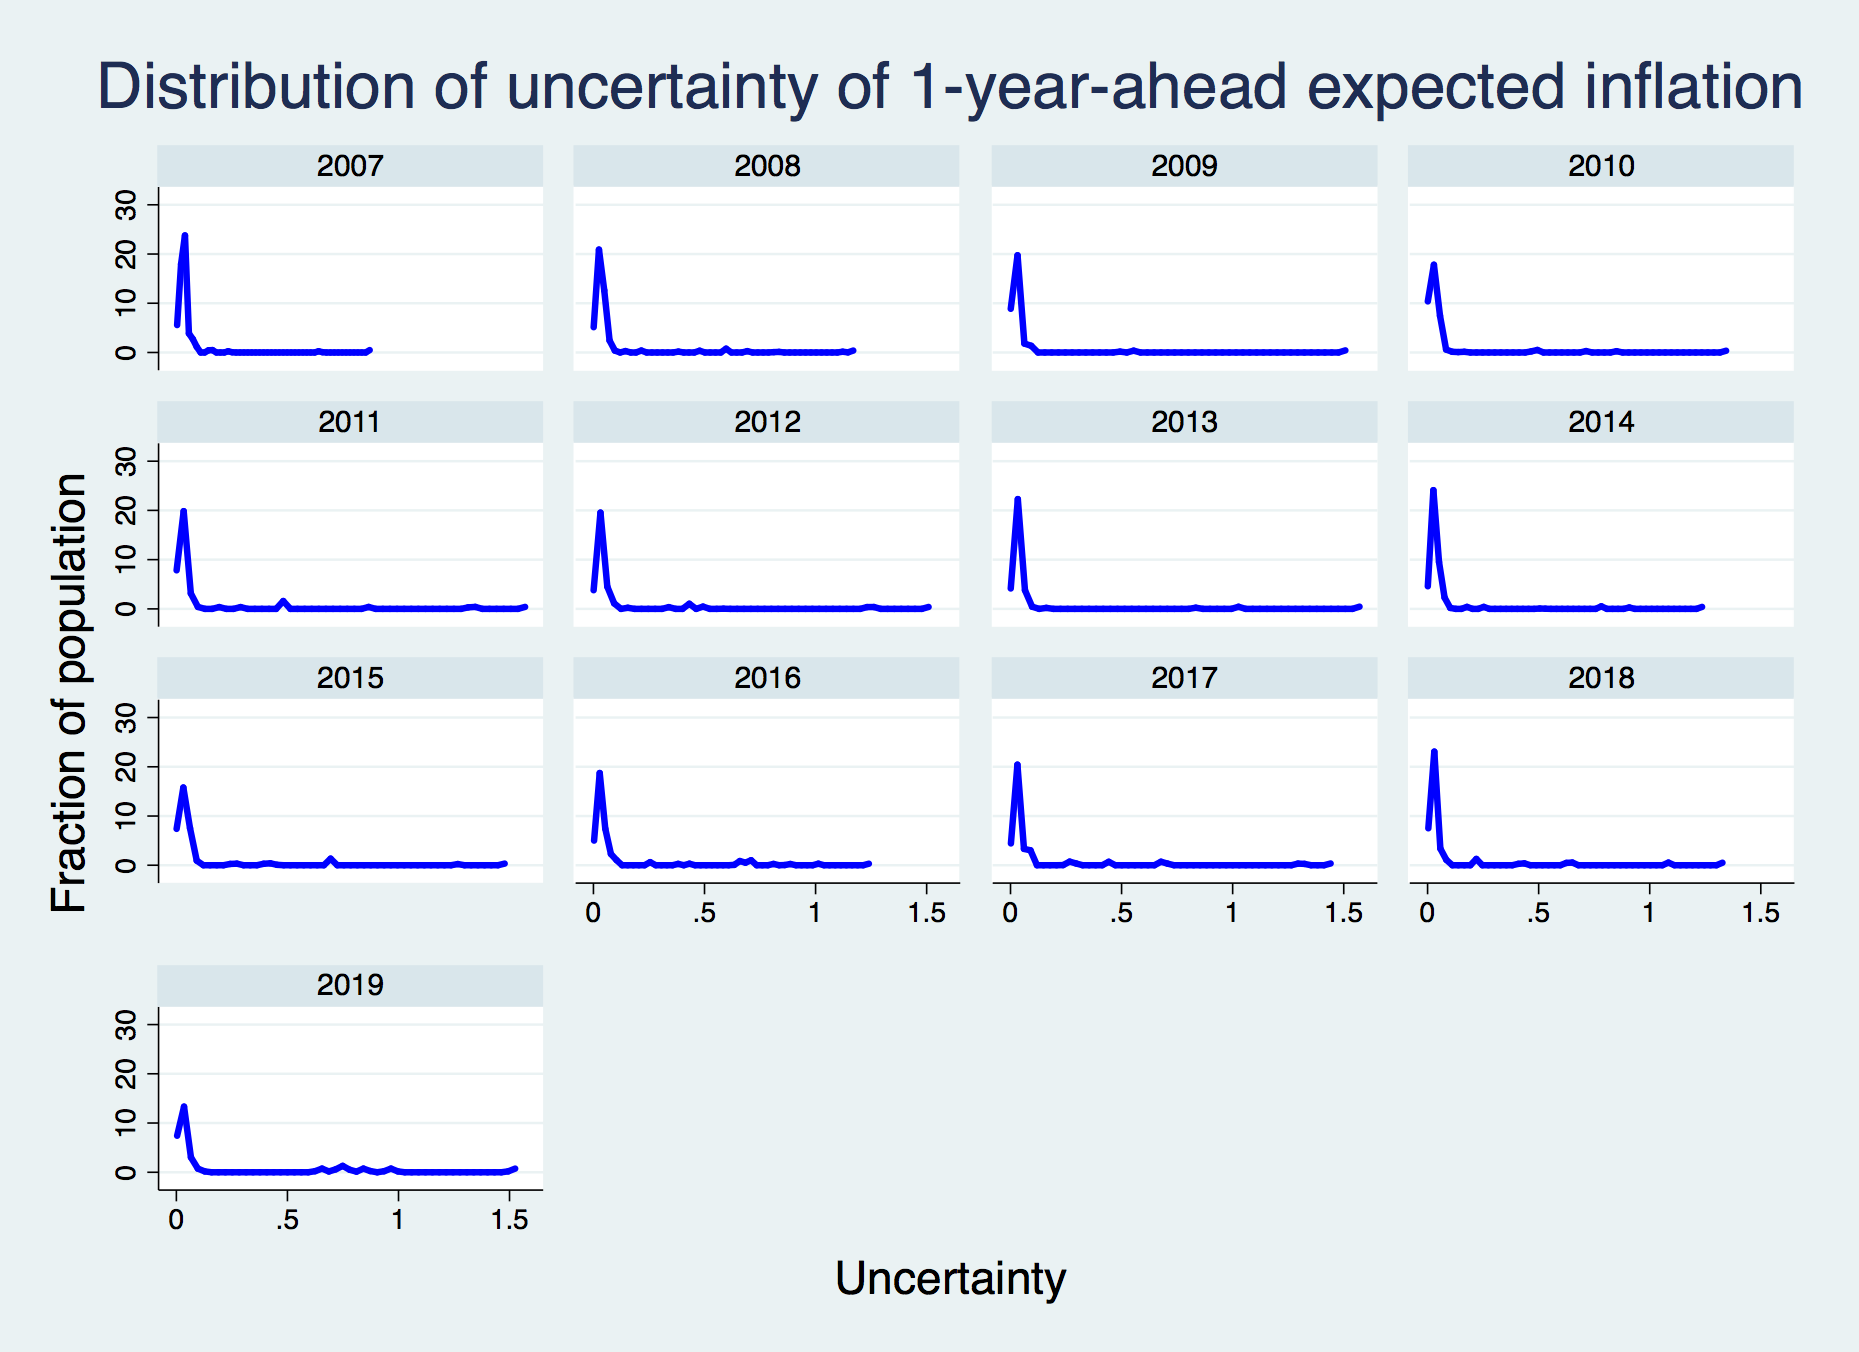
\includegraphics[width=0.33\textwidth]{figuresDraft/PRCCPIVar1_hist.png}  
\smallskip
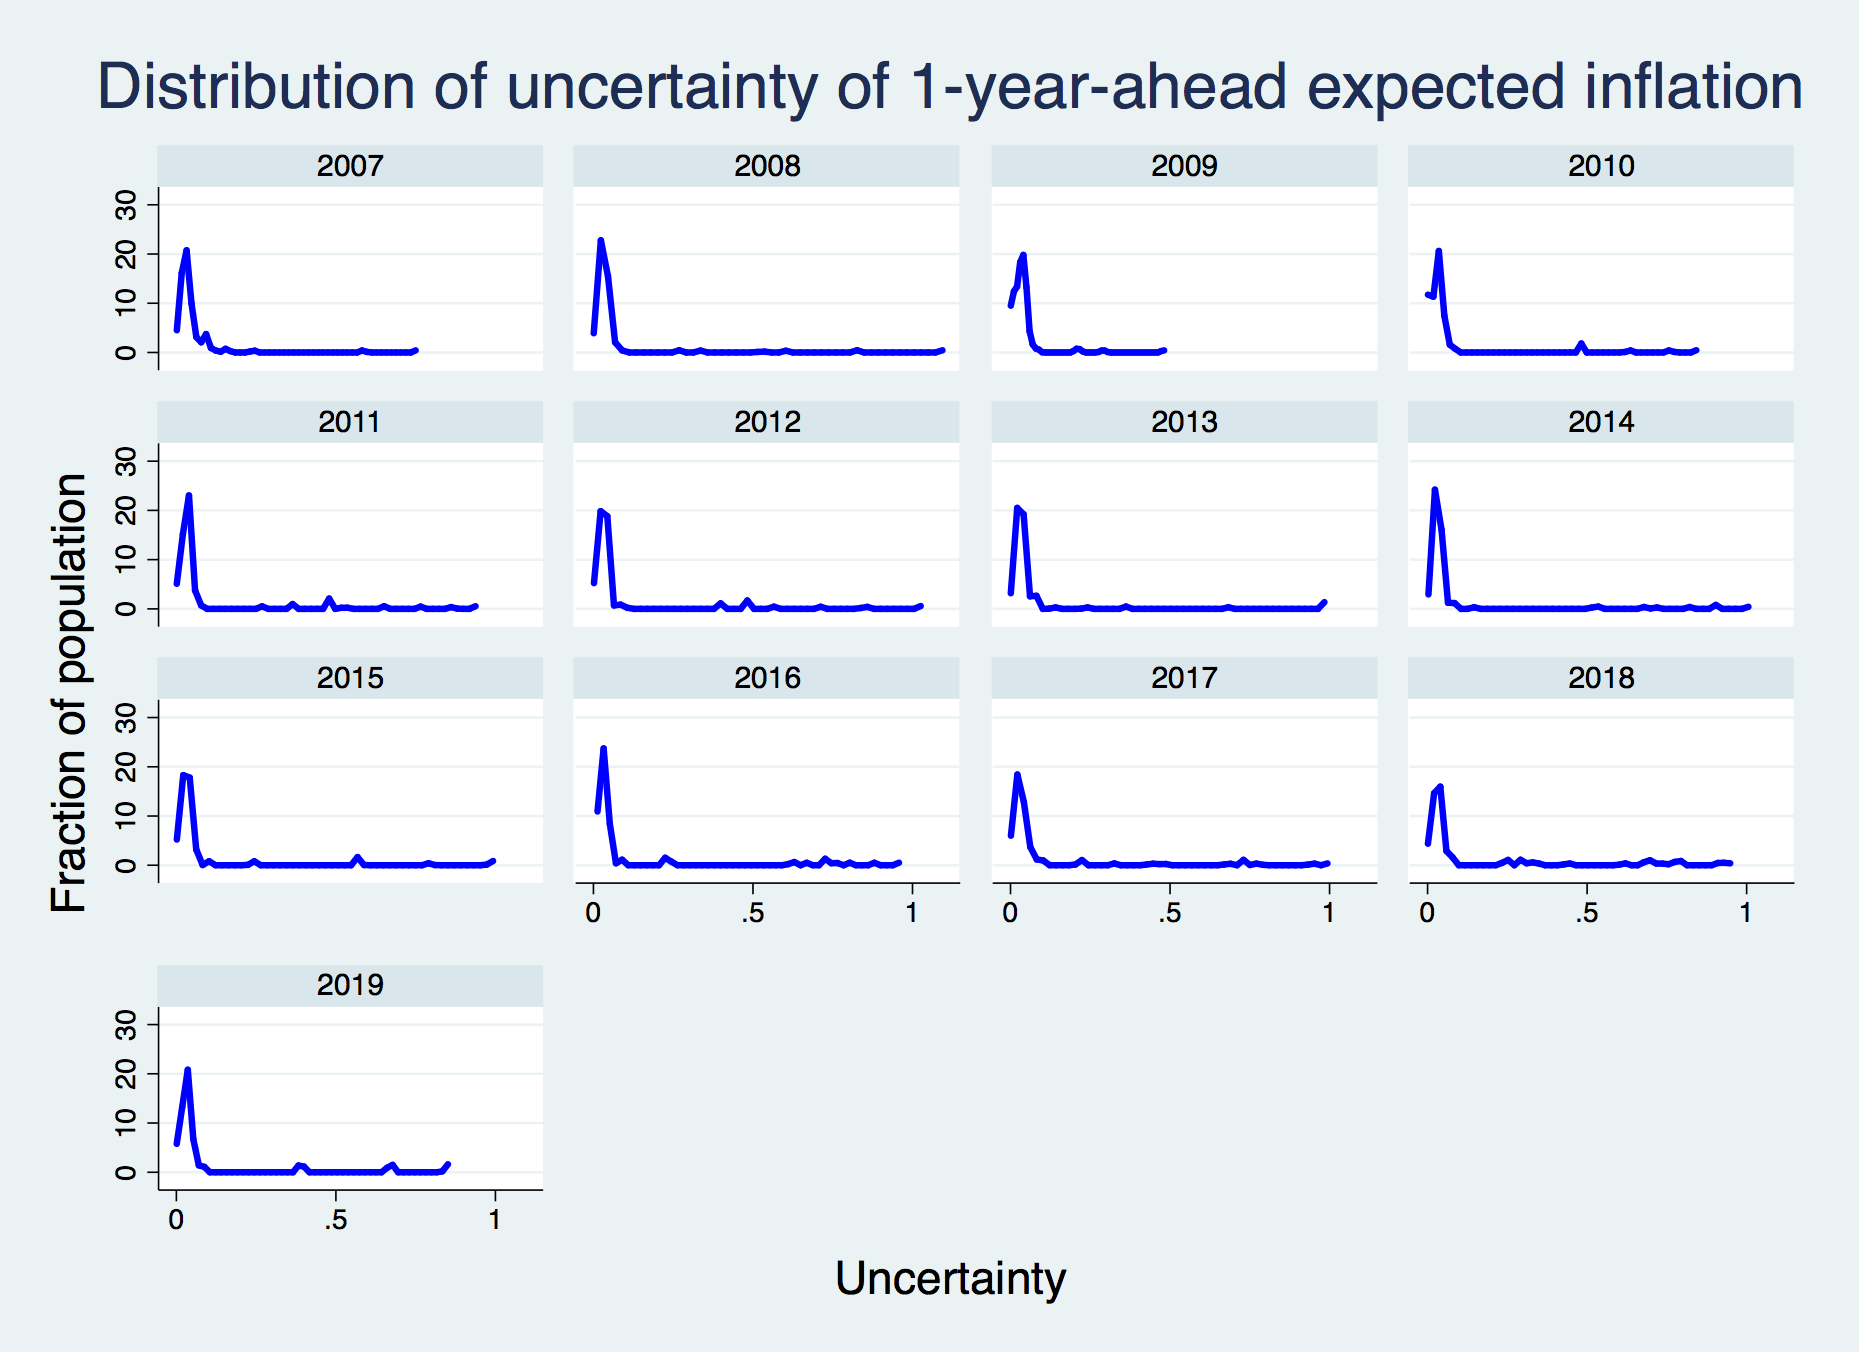
\includegraphics[width=0.33\textwidth]{figuresDraft/PRCPCEVar1_hist.png}  
\smallskip
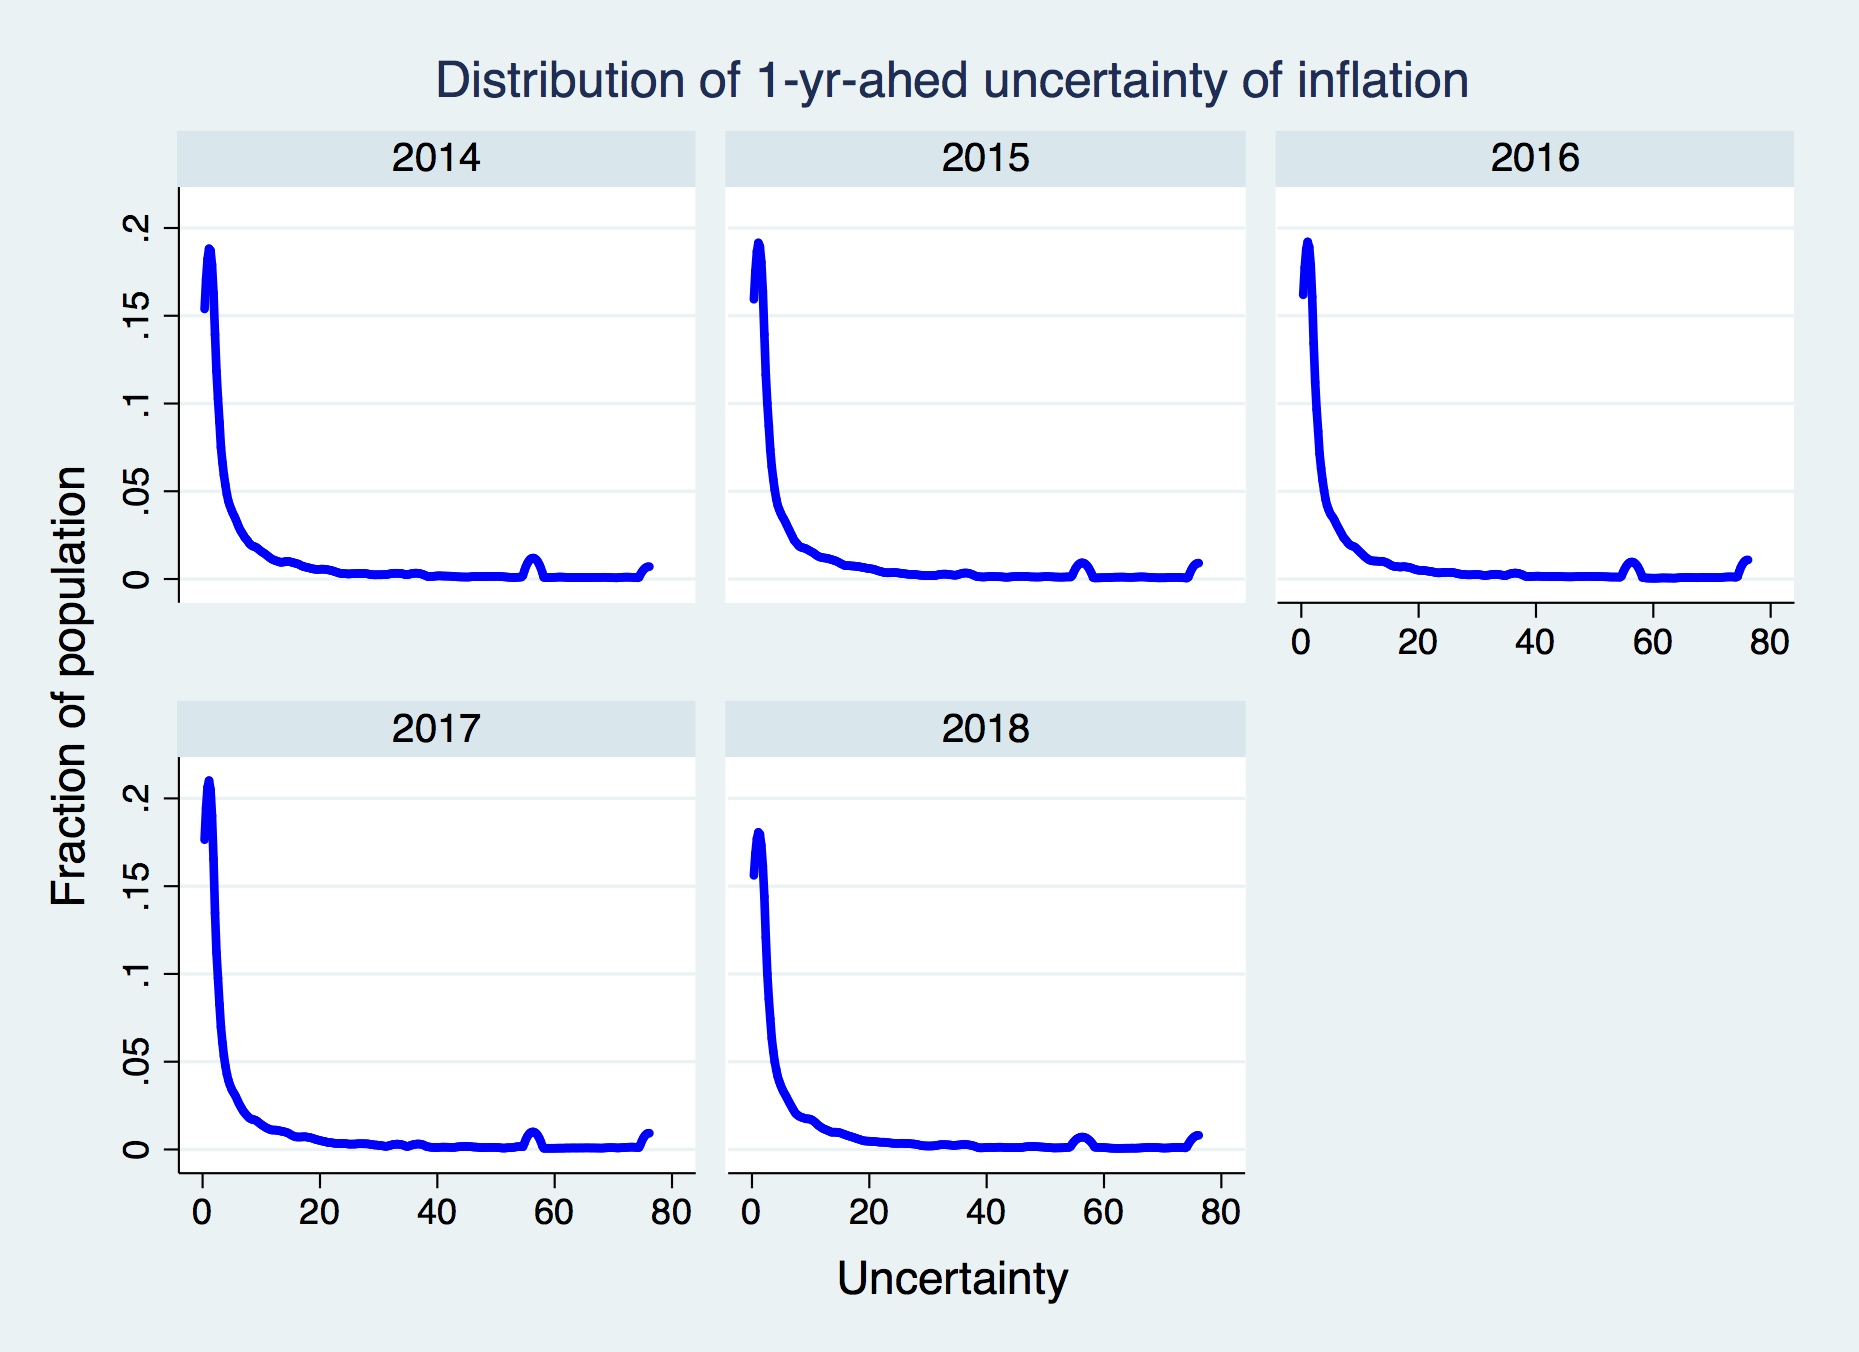
\includegraphics[width=0.33\textwidth]{figuresDraft/SCEvar_hist.png}  
\end{figure}
\end{frame}


\begin{frame}{Distribution of Revision in Forecast}
\begin{figure}
	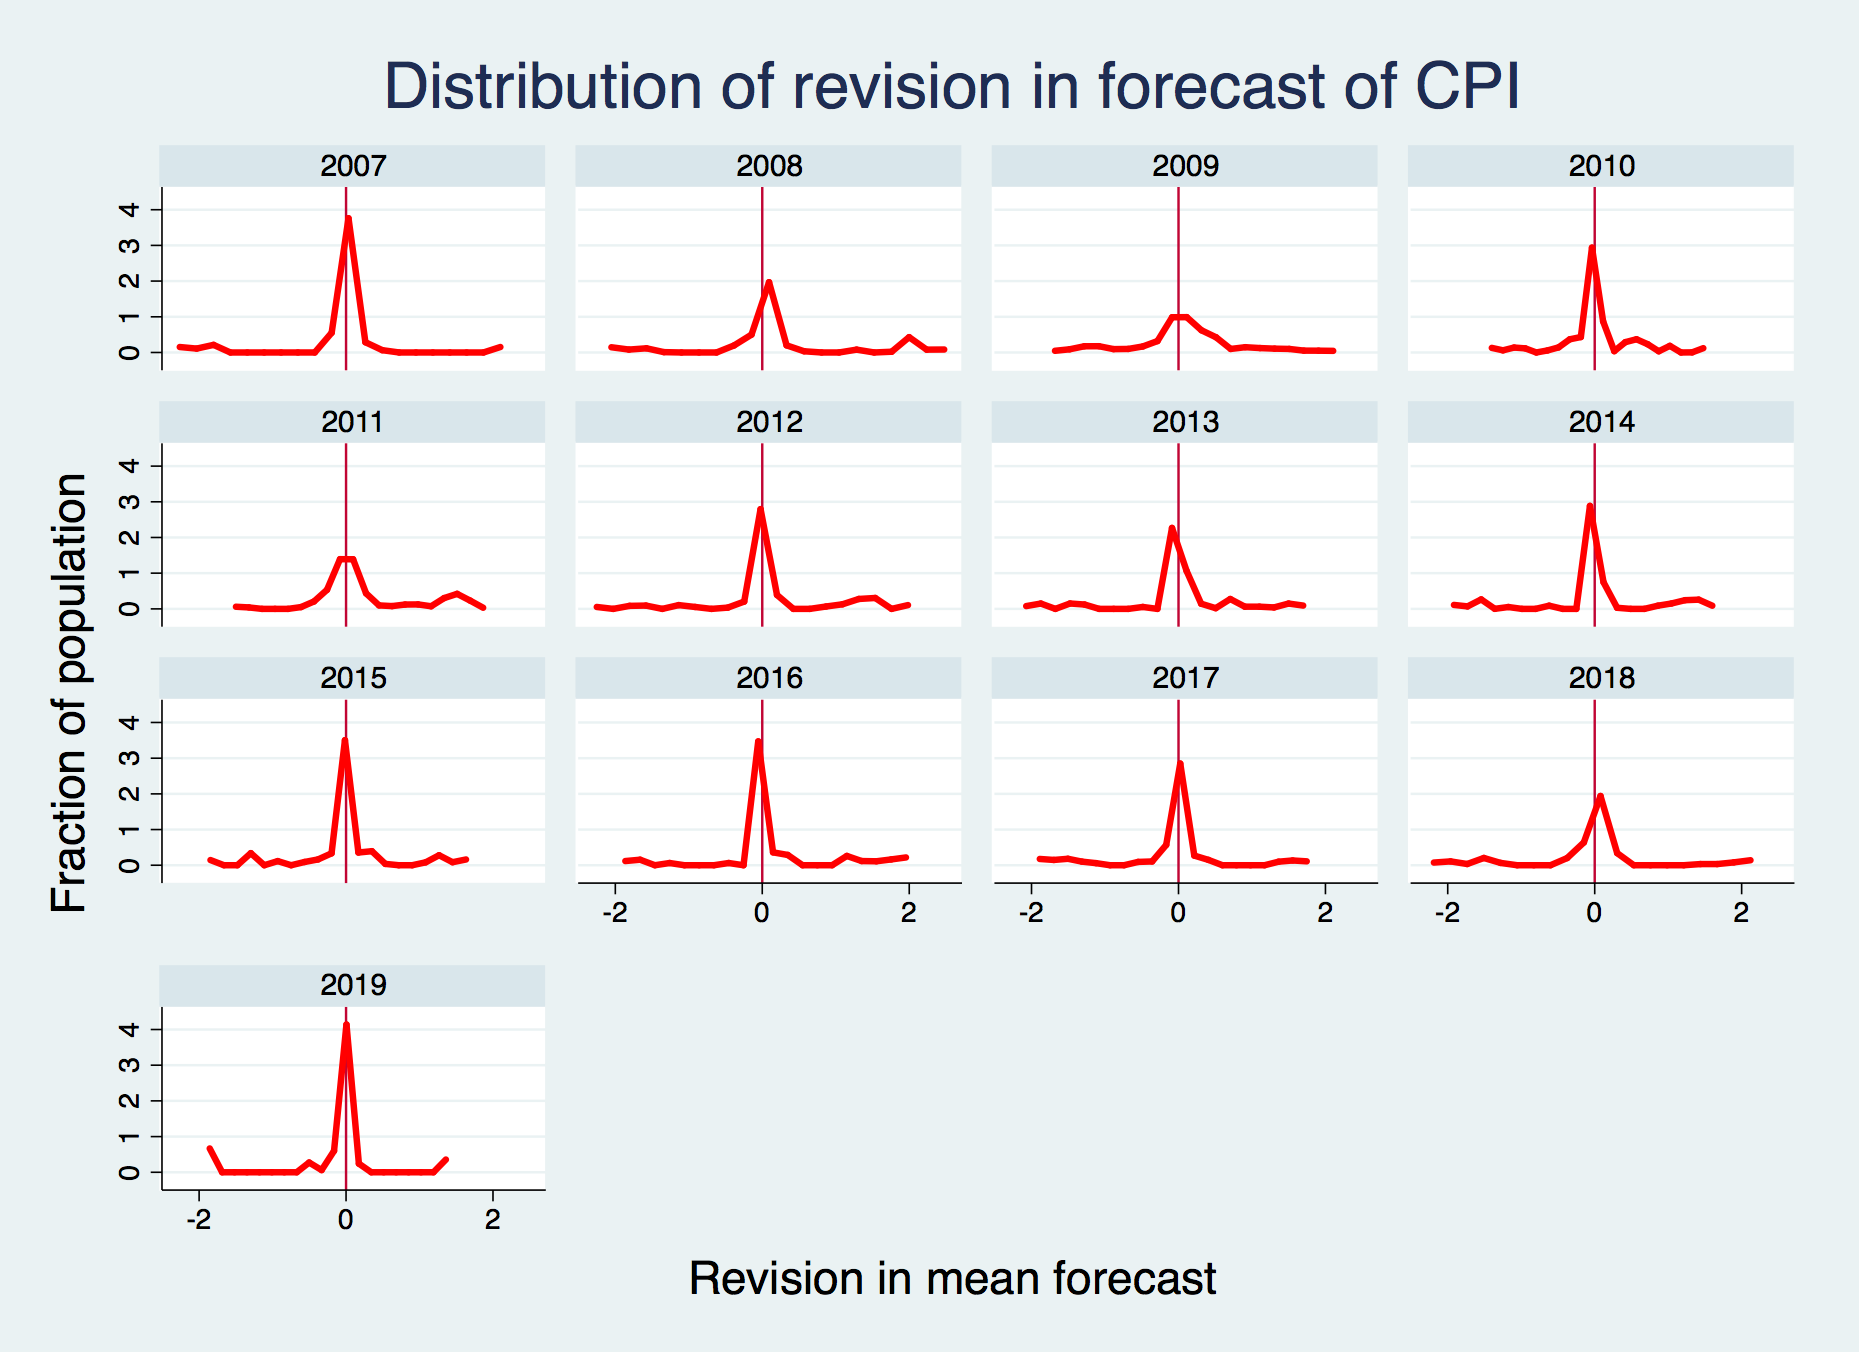
\includegraphics[width=0.5\textwidth]{figuresDraft/PRCCPIMean01_rv_true_hist.png} 
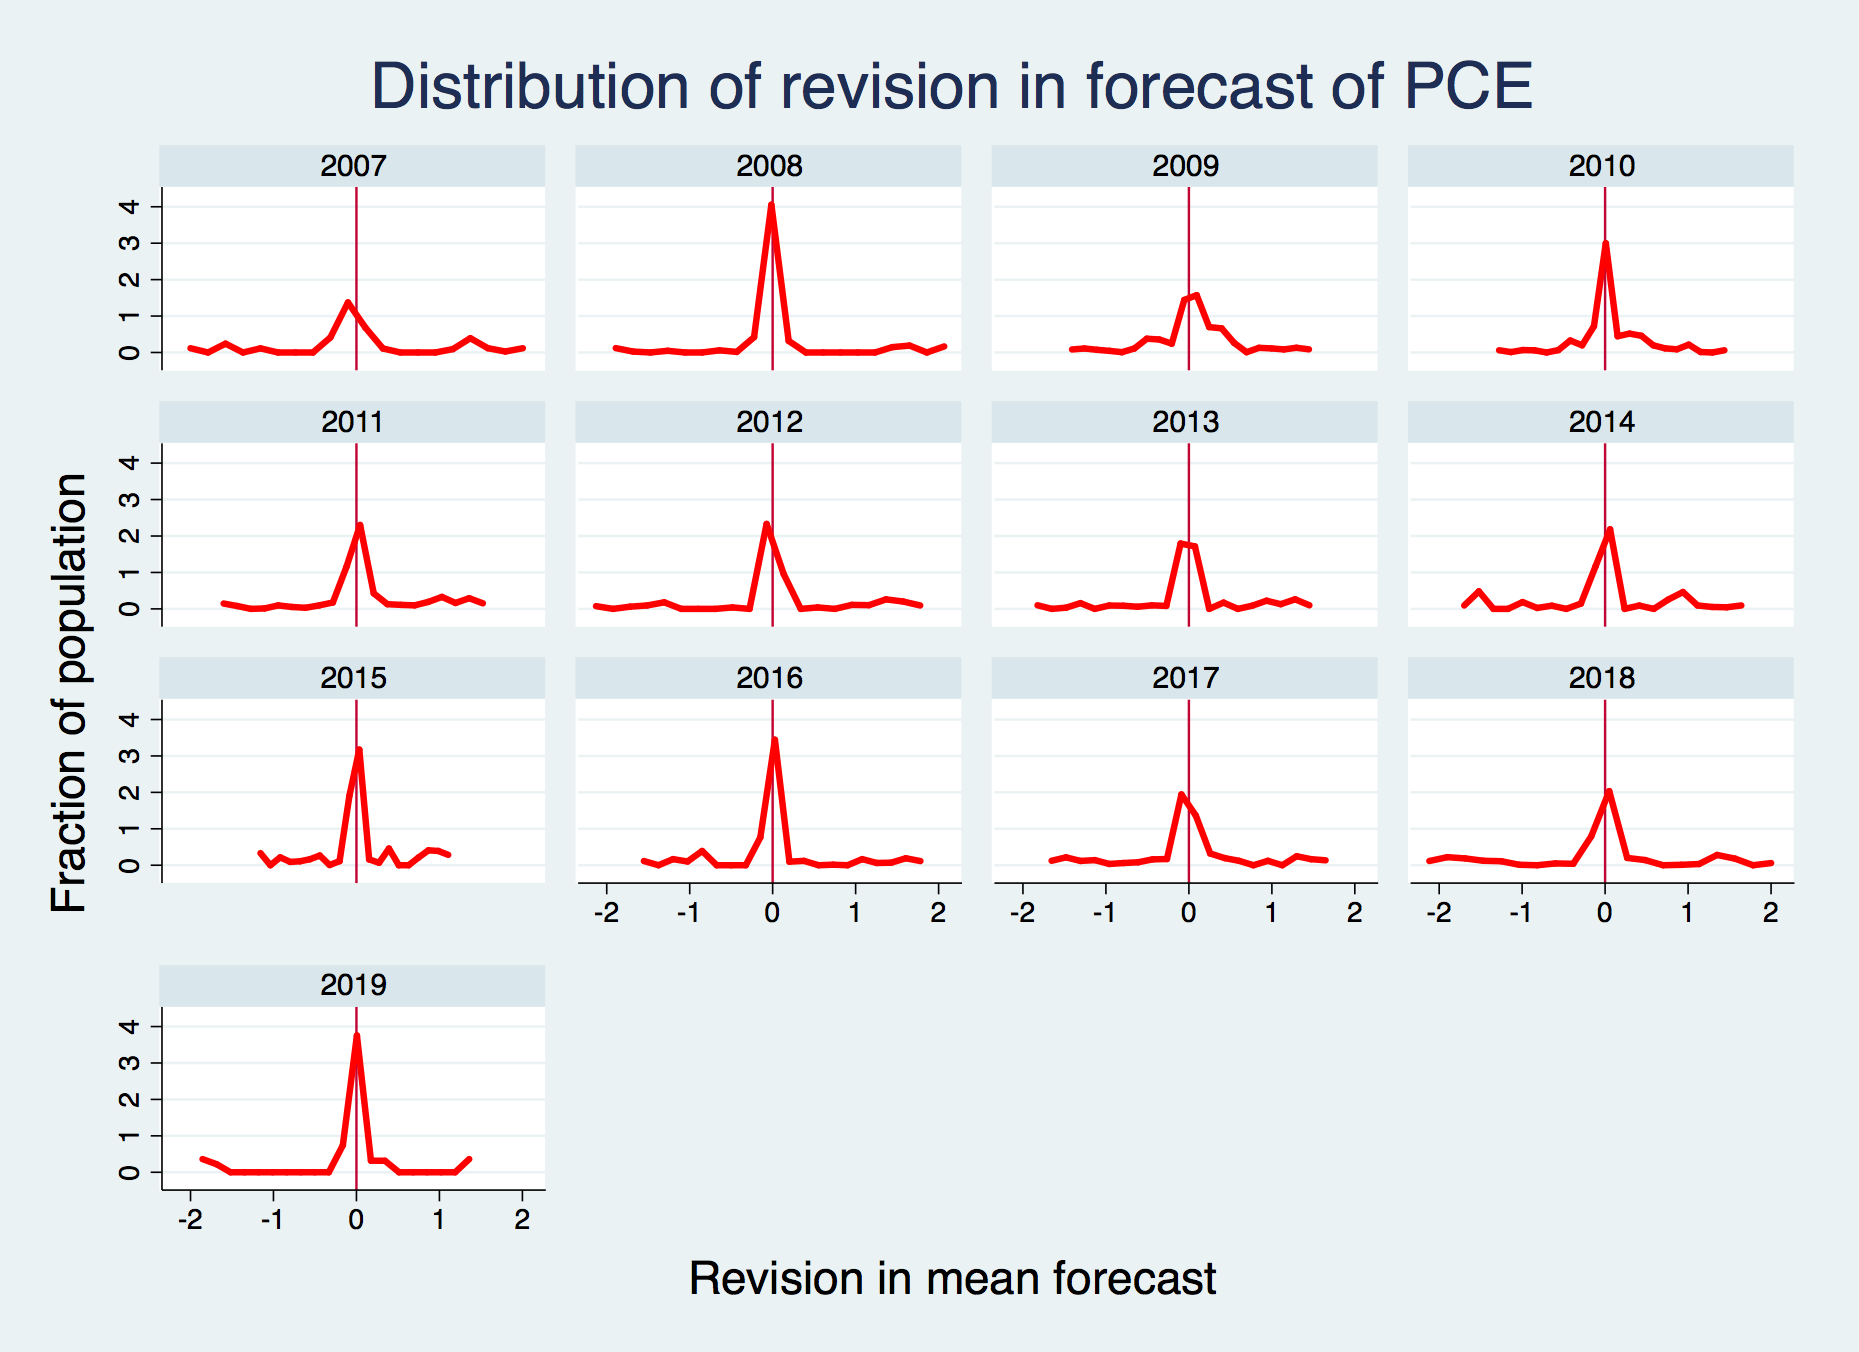
\includegraphics[width=0.5\textwidth]{figuresDraft/PRCPCEMean01_rv_true_hist.png} 
\end{figure}
\end{frame}


\begin{frame}{Distribution of Revision in Uncertainty}
\begin{figure}
	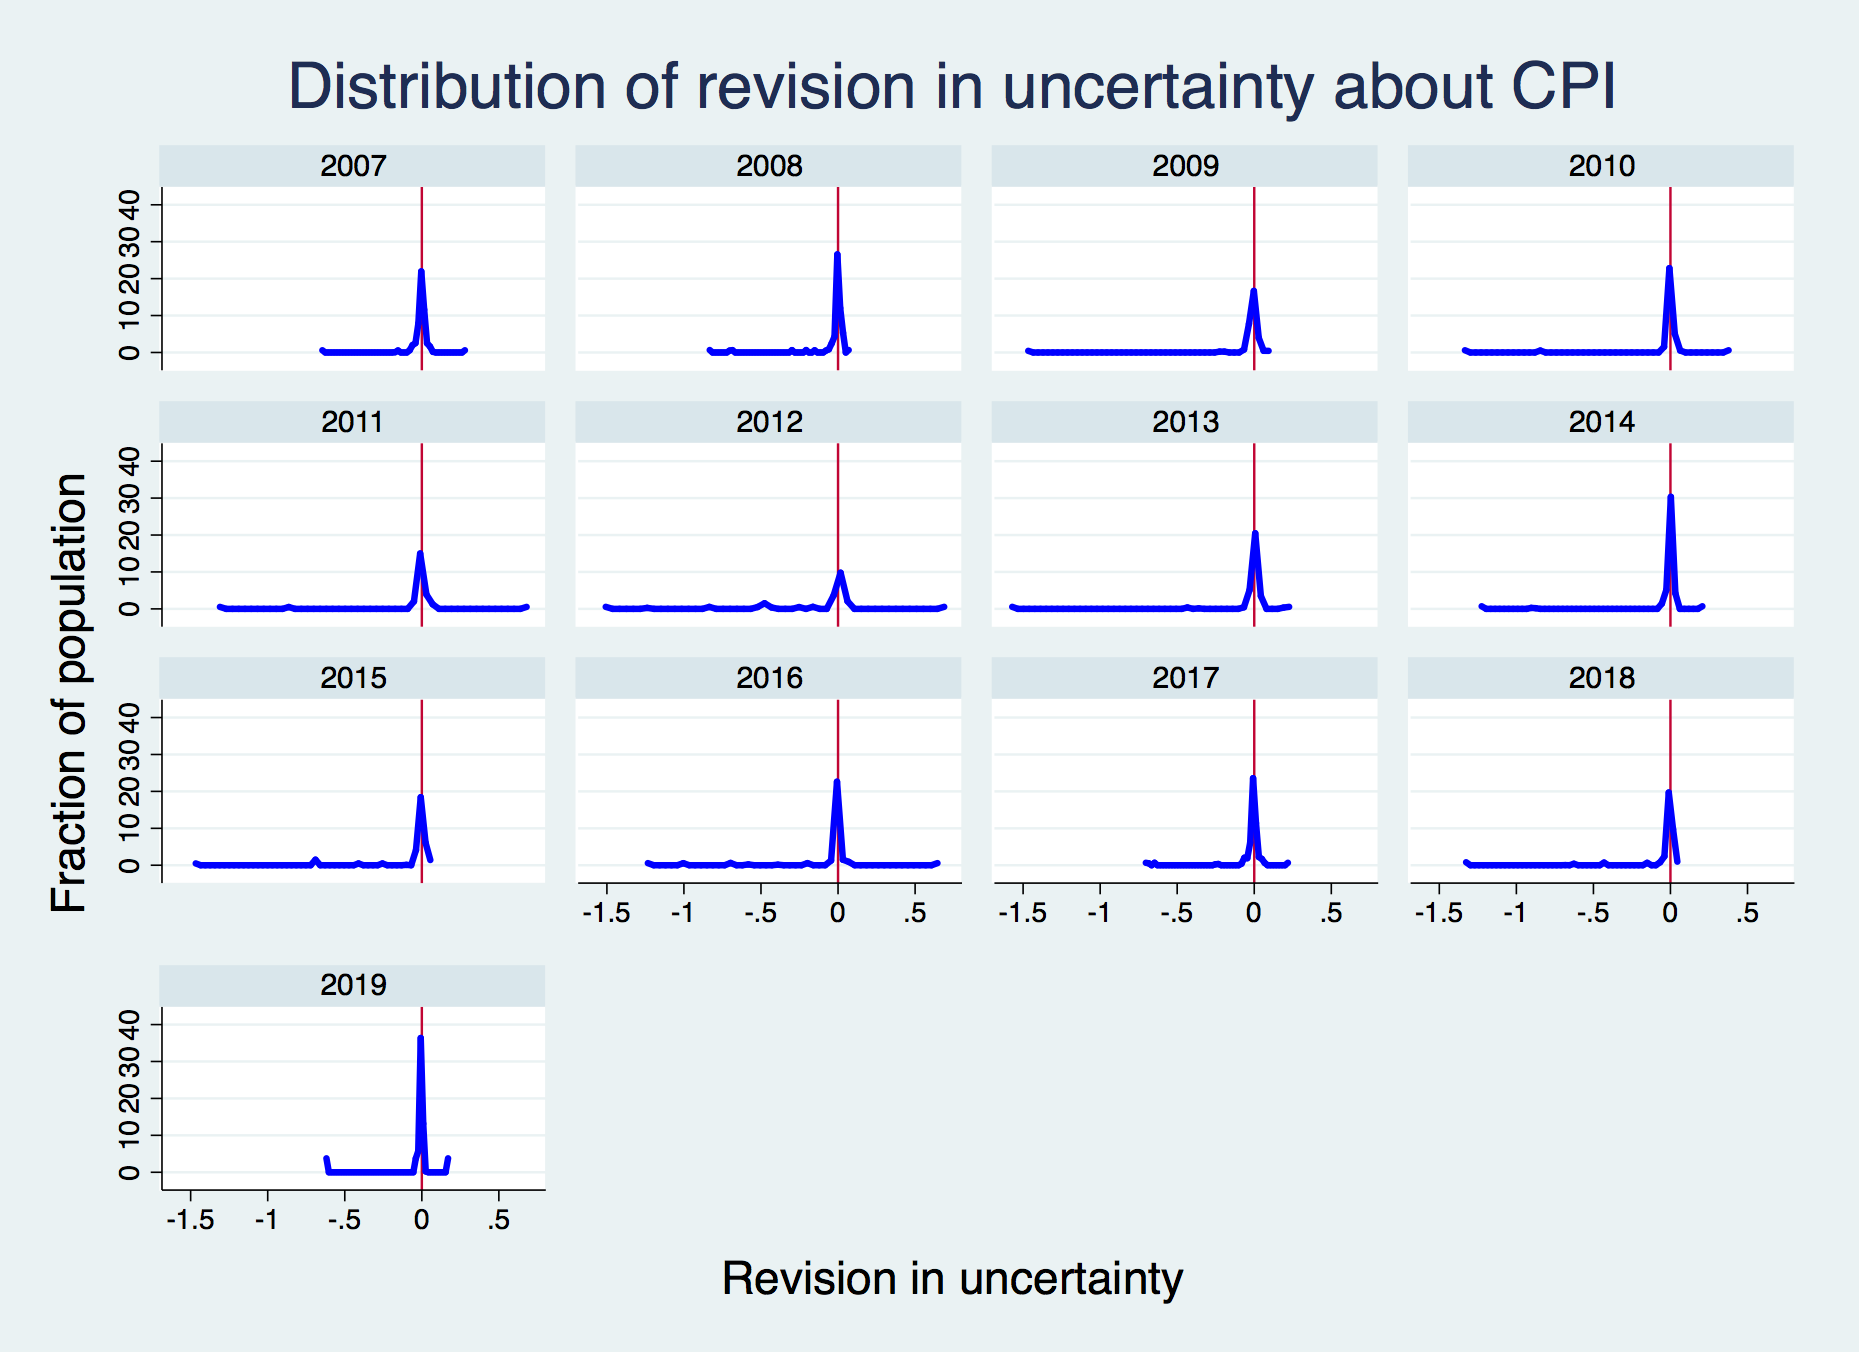
\includegraphics[width=0.5\textwidth]{figuresDraft/PRCCPIVar01_rv_true_hist.png}  
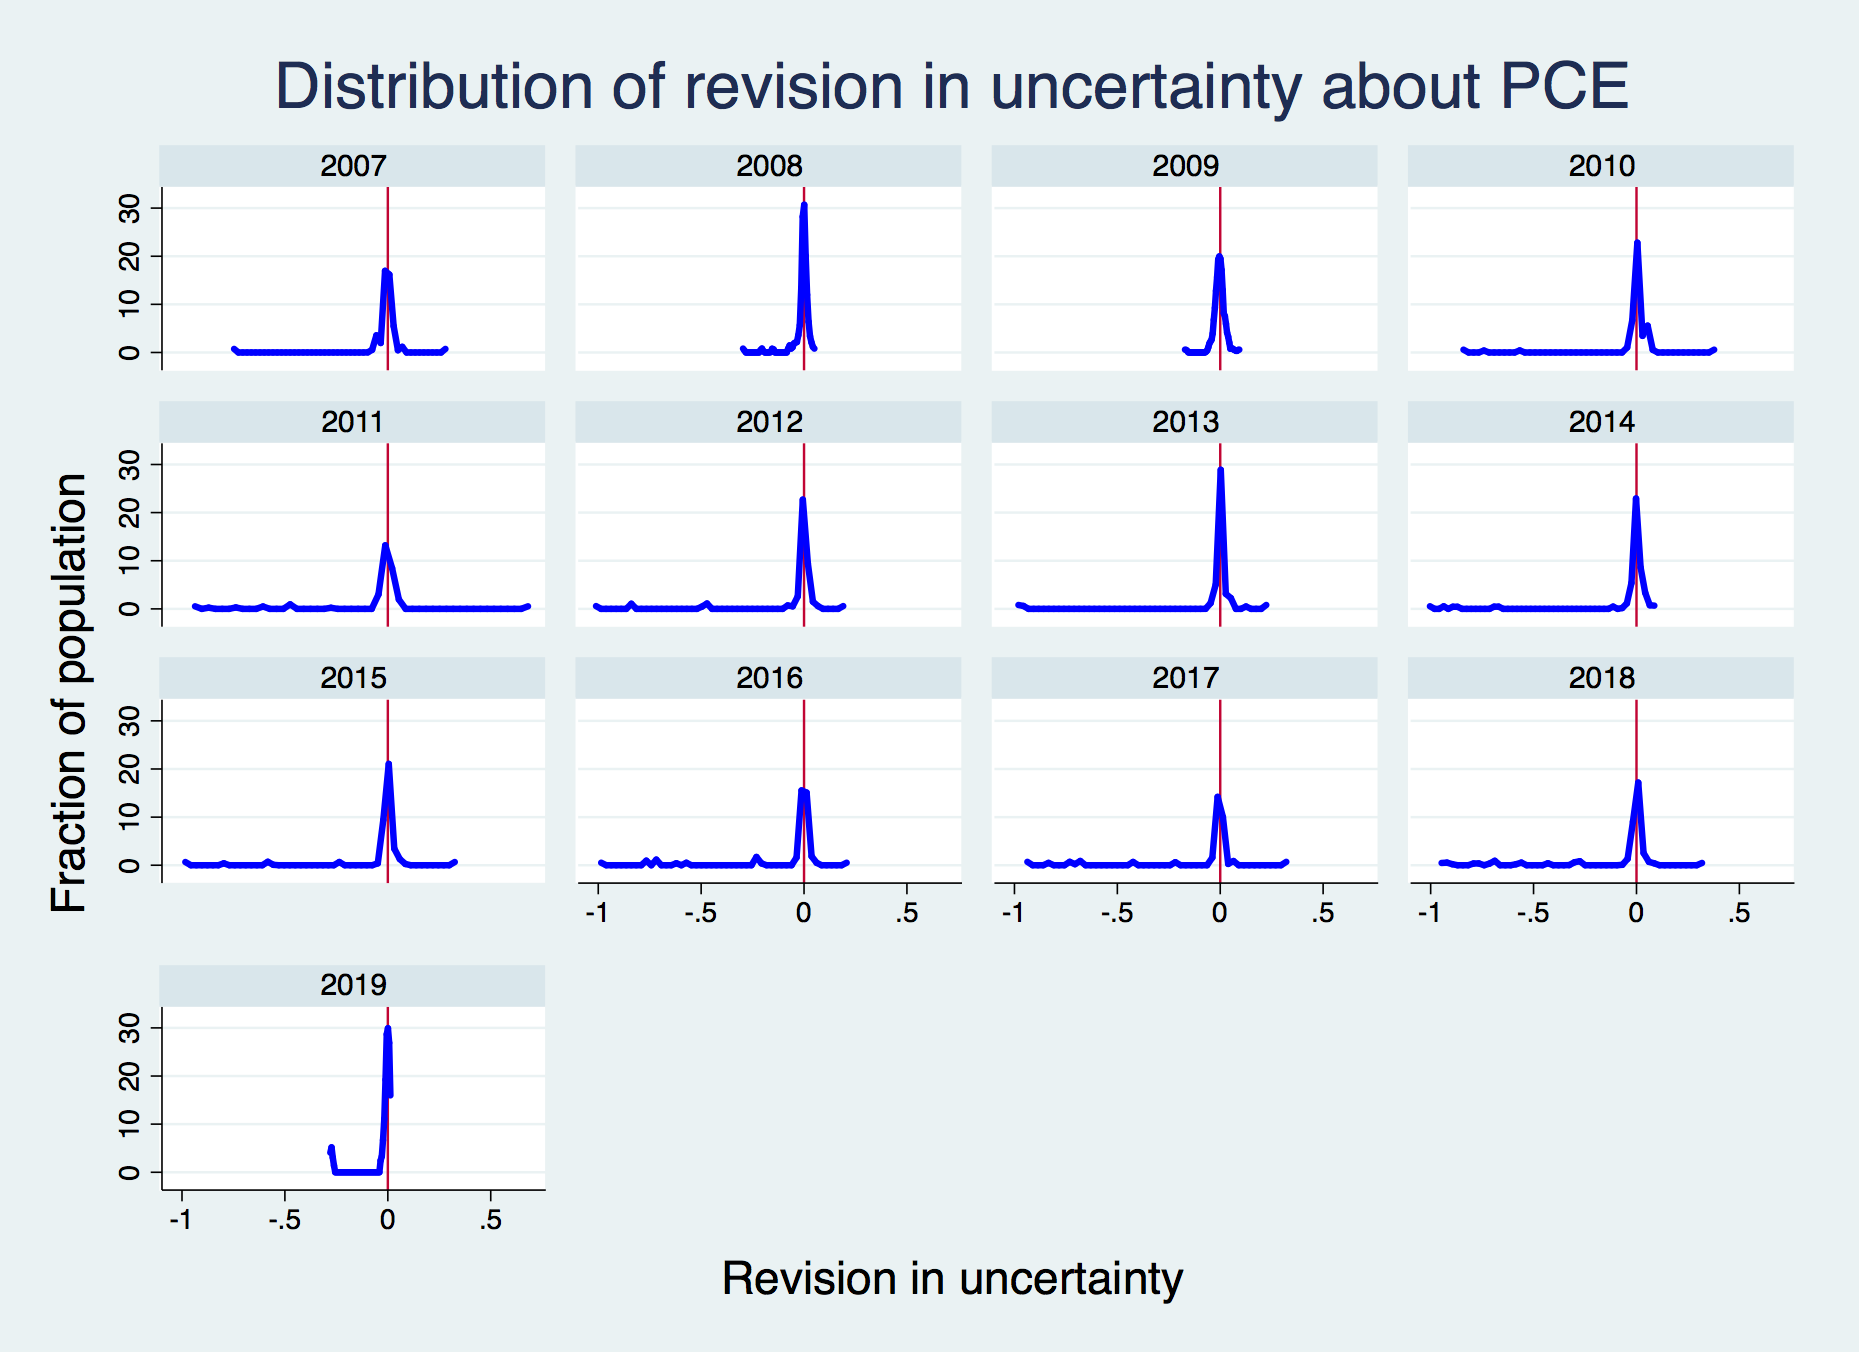
\includegraphics[width=0.5\textwidth]{figuresDraft/PRCPCEVar01_rv_true_hist.png} 
\end{figure}
\end{frame}



\section{Empirical Results}

\begin{frame}{Empirical execution}

\begin{itemize}

\item \textbf{Density Estimation}: generalized beta estimation, \citet{engelberg2009comparing}
 \item \textbf{Identification of Shocks}: following \citet{coibion2012can} and monetary policy shocks. 
\end{itemize}

\end{frame}

\subsection{Test of Null Hypothesis of Rational Expectation}

\begin{frame}{Tests of rationality using forecast errors}
	\begin{adjustbox}{totalheight=0.9\textheight}
	\label{NullTestTable}
	\centering 
	\begin{tabular}{llll}
		\hline 
		& SPF CPI          & SPF PCE          & SCE            \\
		\hline 
		\multicolumn{4}{l}{Test 1: Unbiasedness}                                                           \\
		\hline 
		Constant                            & 0.122***         & 0.586***         & 2.220***       \\
		& (0.017)          & (0.061)          & (0.019)        \\
		\hline 
		N                                   & 4697             & 1208             & 67380          \\
		\hline 
		\multicolumn{4}{l}{Test 2: FE does not depend on past information}                                  \\
		\hline 
		Forecast 1-yr before                & 0.307***         & 0.586***         & NA             \\
		& (0.020)          & (0.061)          & NA             \\
		Constant                            & -0.655***        & -0.777***        & NA             \\
		& (0.060)          & (0.116)          & NA             \\
		\hline 
		N                                   & 3429             & 1208             & NA             \\
		$R^2$                 & 0.0721           & 0.118            & NA             \\
		\hline 
		\multicolumn{4}{l}{Test 3: FEs of non-overlapping forecast horizons not serially correlated} \\
		\hline 
		Forecast Error 1-year before        & 0.0756***        & 0.0503***        & NA             \\
		& (0.020)          & (0.035)          & NA             \\
		Constant                            & 0.145***         & 0.275***         & NA             \\
		& (0.021)          & (0.035)          & NA             \\
		\hline 
		N                                   & 3356             & 1208             & NA             \\
		$R^2$                   & 0.00591          & 0.00264          & NA             \\
		\hline 
		\multicolumn{4}{l}{Test 4: Overlapping FEs are only weakly serially correlated}                          \\
		\hline 
		Forecast Error 1-q before           & 0.657***         & 0.834***         & 0.297***       \\
		& (0.025)          & (0.037)          & (0.021)        \\
		Forecast Error 2-q before           & 0.0282           & -0.0858          & 0.308***       \\
		& (0.027)          & (0.048)          & (0.046)        \\
		Forecast Error 3-q before           & -0.0244          & -0.0555          & 0.311***       \\
		& (0.025)          & (0.038)          & (0.045)        \\
		Constant                            & 0.0626***        & 0.113***         & 0.742***       \\
		& (0.019)          & (0.026)          & (0.097)        \\
		\hline 
		N                                   & 2536             & 1004             & 2836           \\
		$R^2$                & 0.439            & 0.552            & 0.232    \\
		\hline      
	\end{tabular}
\end{adjustbox}

\end{frame}

\begin{frame}{Test of revision efficiency Using mean revisions}

	\begin{adjustbox}{width=0.9\textwidth}
	\begin{threeparttable}
		\label{MeanRevEfficiency}
		\begin{tabular}{lllllllll}
			\hline 
			& \multicolumn{4}{l}{SPF CPI}                     & \multicolumn{4}{l}{SPF PCE}                       \\
			\hline 
			\multicolumn{9}{l}{Test 1.  Revision efficiency of mean forecast}            \\
			\hline 
			& Mean revision & t-1       & t-1- t-2 & t-1-t-3  & Mean revision & t-1       & t-1- t-2  & t-1-t-3   \\
			\hline 
			L.InfExp\_Mean\_rv  &               & 0.539***  & 0.418*** & 0.387*** &               & 0.606***  & 0.435***  & 0.369***  \\
			&               & (0.031)   & (0.043)  & (0.052)  &               & (0.034)   & (0.042)   & (0.049)   \\
			L2.InfExp\_Mean\_rv &               &           & 0.218*** & 0.166**  &               &           & 0.261***  & 0.246***  \\
			&               &           & (0.040)  & (0.053)  &               &           & (0.047)   & (0.058)   \\
			L3.InfExp\_Mean\_rv &               &           &          & 0.134**  &               &           &           & 0.116     \\
			&               &           &          & (0.048)  &               &           &           & (0.069)   \\
			SPFCPI\_ct50        &               & -0.444*** & -0.391** & -0.454** &               &           &           &           \\
			&               & (0.105)   & (0.124)  & (0.138)  &               &           &           &           \\
			SPFPCE\_ct50        &               &           &          &          &               & -0.432*** & -0.413*** & -0.504*** \\
			&               &           &          &          &               & (0.109)   & (0.111)   & (0.138)   \\
			& -1.257***     & 0.329     & 0.351    & 0.546*   & -1.095***     & 0.365     & 0.428*    & 0.641**   \\
			Constant & (0.045)       & (0.191)   & (0.237)  & (0.269)  & (0.039)       & (0.188)   & (0.191)   & (0.228)   \\
			\hline 
			N                   & 1337          & 1045      & 822      & 652      & 1111          & 867       & 683       & 549       \\
			$R^2$                  & 0.000         & 0.335     & 0.355    & 0.372    & 0.000         & 0.409     & 0.444     & 0.452     \\
			\hline 
		\end{tabular} 
		\begin{tablenotes}
			\item Standard errors are clustered by date. *** p$<$0.001, ** p$<$0.01 and * p$<$0.05.
		\end{tablenotes}
	\end{threeparttable}
\end{adjustbox}

\end{frame}


\begin{frame}{Test of revision efficiency using uncertainty revisions}

\begin{adjustbox}{width=0.9\textwidth}
	\begin{threeparttable}
		\label{VarRevEfficiency}
		\begin{tabular}{lllllllll}
			\hline 
			& \multicolumn{4}{l}{SPF CPI}                     & \multicolumn{4}{l}{SPF PCE}                       \\
			\hline 
			\multicolumn{9}{l}{Test 2. Revision efficiency of uncertainty}                                                            \\
			\hline 
			& Mean revision & t-1       & t-1- t-2 & t-1-t-3  & Mean revision & t-1       & t-1- t-2  & t-1-t-3   \\
			\hline 
			L.InfExp\_Var\_rv   &               & 0.290*    & 0.529*** & 0.581*** &               & 0.577***  & 0.477***  & 0.344*    \\
			&               & (0.122)   & (0.117)  & (0.145)  &               & (0.080)   & (0.130)   & (0.148)   \\
			L2.InfExp\_Var\_rv  &               &           & -0.059   & -0.209   &               &           & 0.360*    & 0.205*    \\
			&               &           & (0.125)  & (0.127)  &               &           & (0.143)   & (0.098)   \\
			L3.InfExp\_Var\_rv  &               &           &          & 0.353**  &               &           &           & 0.390*    \\
			&               &           &          & (0.121)  &               &           &           & (0.149)   \\
			Constant              & -0.034***     & -0.011**  & -0.008*  & -0.005   & -0.039***     & -0.019**  & -0.010**  & -0.007*   \\
			& (0.005)       & (0.004)   & (0.003)  & (0.004)  & (0.006)       & (0.006)   & (0.003)   & (0.003)   \\
			\hline 
			N                   & 1189          & 877       & 663      & 504      & 1082          & 801       & 604       & 458       \\
			$R^2$                 & 0.000         & 0.124     & 0.284    & 0.408    & 0.000         & 0.353     & 0.583     & 0.723    \\
			\hline 
		\end{tabular} 
		\begin{tablenotes}
			\item Standard errors are clustered by date. *** p$<$0.001, ** p$<$0.01 and * p$<$0.05.
		\end{tablenotes}
	\end{threeparttable}
\end{adjustbox}

\end{frame}


\begin{frame}{Weak tests of efficiency using changes in forecasts }

	\begin{adjustbox}{width=\textwidth}
	\begin{threeparttable}
		\caption{Weak Tests of Revision Efficiency using Change in Forecasts and Uncertainty}
		\label{MeanWeakRevEfficiency}
		\begin{tabular}{llllllllllllll}
			\hline 
			& \multicolumn{4}{l}{SPF CPI}                     & \multicolumn{4}{l}{SPF PCE}                       &                      & \multicolumn{4}{l}{SCE}                           \\
			\hline 
			\multicolumn{14}{l}{Test 3. Weak revision efficiency of change in forecast}                                                                                                                                    \\
			\hline 
			& Mean change & t-1       & t-1- t-2  & t-1-t-3   & Mean revision & t-1       & t-1- t-2  & t-1-t-3   &                      & Mean revision & t-1       & t-1- t-2  & t-1-t-3   \\
			\hline 
			L.InfExp\_Mean\_ch   &             & -0.295*** & -0.344*** & -0.367*** &               & -0.303*** & -0.348*** & -0.364*** & L.InfExp\_Mean\_ch  &         & -0.433*** & -0.586*** & -0.642*** \\
			&             & (0.034)   & (0.044)   & (0.045)   &               & (0.043)   & (0.059)   & (0.062)   &                    &         & (0.01)     & (0.013)    & (0.025)    \\
			
			L2.InfExp\_Mean\_ch  &             &           & -0.179*** & -0.242*** &               &           & -0.162*   & -0.200**  & L2.InfExp\_Mean\_ch &         &           & -0.336*** & -0.439*** \\
			
			&             &           & (0.047)   & (0.049)   &               &           & (0.061)   & (0.067)   &                                   &         &           & (0.018)    & (0.031)    \\
			L3.InfExp\_Mean\_ch  &             &           &           & -0.097**  &               &           &           & -0.088*   & L3.InfExp\_Mean\_ch &         &           & -0.143*** & -0.270*** \\
			
			&             &           &           & (0.032)   &               &           &           & (0.036)   &                                &         &           & (0.012)    & (0.027)    \\
			
			&             &           &           &           &               &           &           &           & L4.InfExp\_Mean\_ch &         &           &           & -0.183*** \\
			
			&             &           &           &           &               &           &           &           &                                 &         &           &           & (0.027)    \\
			&             &           &           &           &               &           &           &           & L5.InfExp\_Mean\_ch &         &           &           & -0.096*** \\
			&             &           &           &           &               &           &           &           &                      &         &           &           & (0.021)    \\
			&             &           &           &           &               &           &           &           & L6.InfExp\_Mean\_ch &         &           &           & -0.044**  \\
			&             &           &           &           &               &           &           &           &                                     &         &           &           & (0.013)    \\
			Constant               & -0.005      & -0.004    & -0.011    & -0.015    & 0.001         & 0.008     & -0.002    & -0.007    & Constant              & -0.055* & -0.034    & -0.001    & -0.002    \\
			& (0.023)     & (0.024)   & (0.026)   & (0.026)   & (0.020)       & (0.020)   & (0.022)   & (0.022)   &                                 & -0.023  & -0.023    & -0.028    & -0.033    \\
			\hline 
			N                    & 1636        & 1430      & 1266      & 1141      & 1402          & 1190      & 1022      & 898       & N                   & 53016   & 43166     & 28850     & 14445     \\
			$R^2$                  & 0.000       & 0.086     & 0.112     & 0.128     & 0.000         & 0.090     & 0.112     & 0.120     & $R^2$ &  0.000       & 0.202     & 0.273     & 0.306   \\
			\hline 
		\end{tabular}
		\begin{tablenotes}
			\item Standard errors are clustered by date. *** p$<$0.001, ** p$<$0.01 and * p$<$0.05.
		\end{tablenotes}
	\end{threeparttable}
\end{adjustbox}
\end{frame}

\begin{frame}{Weak Tests of Efficiency using changes in uncertainty}
\begin{adjustbox}{width=\textwidth}
	\begin{threeparttable}
				\label{VarWeakRevEfficiency}
		\begin{tabular}{llllllllllllll}
			\hline 
			& \multicolumn{4}{l}{SPF CPI}                     & \multicolumn{4}{l}{SPF PCE}                       &                      & \multicolumn{4}{l}{SCE}                           \\
			\hline 
			\multicolumn{14}{l}{Test 4. Weak revision efficiency of change in uncertainty}                \\
			\hline                                                                                                                 
			& Mean change & t-1       & t-1- t-2  & t-1-t-3   & Mean change   & t-1       & t-1- t-2  & t-1-t-3   &                      & Mean change   & t-1       & t-1- t-2  & t-1-t-3   \\
			\hline 
			L.InfExp\_Var\_ch    &             & -0.393**  & -0.568*** & -0.543**  &               & -0.444*** & -0.602*** & -0.658*** & L.InfExp\_Var\_ch    &               & -0.382*** & -0.565*** & -0.652*** \\
			&             & (0.136)   & (0.146)   & (0.177)   &               & (0.094)   & (0.127)   & (0.145)   &                      &               & -0.015    & -0.022    & -0.037    \\
			L2.InfExp\_Var\_ch   &             &           & -0.322**  & -0.278*   &               &           & -0.289*   & -0.404**  & L2.InfExp\_Var\_ch   &               &           & -0.300*** & -0.406*** \\
			&             &           & (0.104)   & (0.132)   &               &           & (0.110)   & (0.137)   &                      &               &           & -0.021    & -0.031    \\
			L3.InfExp\_Var\_ch   &             &           &           & 0.048     &               &           &           & -0.292    & L3.InfExp\_Var\_ch   &               &           & -0.123*** & -0.265*** \\
			&             &           &           & (0.096)   &               &           &           & (0.154)   &                      &               &           & -0.012    & -0.027    \\
			&             &           &           &           &               &           &           &           & L4.InfExp\_Var\_ch   &               &           &           & -0.130*** \\
			&             &           &           &           &               &           &           &           &                      &               &           &           & -0.025    \\
			&             &           &           &           &               &           &           &           & L5.InfExp\_Var\_ch   &               &           &           & -0.058**  \\
			&             &           &           &           &               &           &           &           &                      &               &           &           & -0.018    \\
			&             &           &           &           &               &           &           &           & L6.InfExp\_Var\_ch   &               &           &           & -0.025    \\
			&             &           &           &           &               &           &           &           &                      &               &           &           & -0.012    \\
			Constant               & -0.002      & -0.001    & 0.004     & 0.004     & 0.000         & 0.002     & 0.004     & 0.005     &   Constant                   & -1.339***     & -1.324*** & -1.139*** & -0.839*** \\
			& (0.005)     & (0.005)   & (0.004)   & (0.004)   & (0.004)       & (0.004)   & (0.004)   & (0.004)   &                      & -0.123        & -0.11     & -0.104    & -0.163    \\
			\hline 
			N                    & 1202        & 950       & 765       & 625       & 1078          & 842       & 657       & 519       &                      & 53016         & 43166     & 28850     & 14445     \\
			$R^2$ & 0.000       & 0.120     & 0.265     & 0.242     & 0.000         & 0.233     & 0.321     & 0.385     &                      & 0             & 0.182     & 0.278     & 0.321  \\
			\hline    
		\end{tabular}
		\begin{tablenotes}
			\item Standard errors are clustered by date. *** p$<$0.001, ** p$<$0.01 and * p$<$0.05.
		\end{tablenotes}
	\end{threeparttable}
\end{adjustbox}
\end{frame}

\begin{frame}{Estimation: minimum distance approach}
	\begin{itemize}
\item model-specific moment dynamics as a function real time data and process parameters 
\item minimize the distance (percent deviation) from the data moments to find the parameter of expectation formation	
	\end{itemize}
\end{frame}

\begin{frame}{Results: professionals and SEAR}
\begin{figure}[ht]
	\centering
    \label{SE_diag_SPF}
		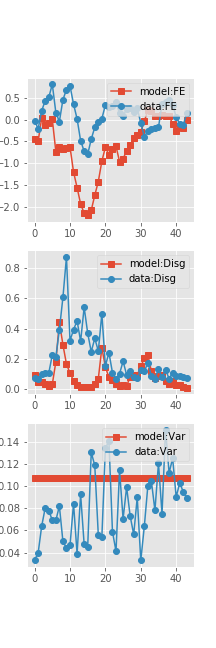
\includegraphics[width=0.19\textwidth, height = \0.95\textheight]{figures/spf_se_est_diag0.png}
		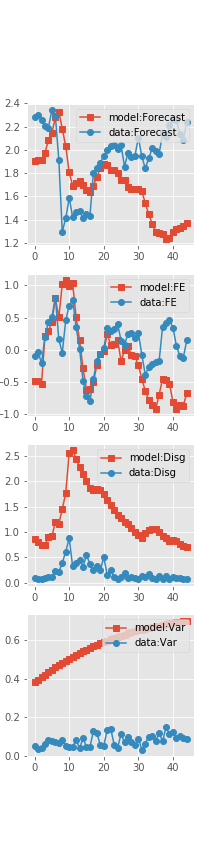
\includegraphics[width=0.19\textwidth, height = \0.95\textheight]{figures/spf_se_est_diag1.png}
		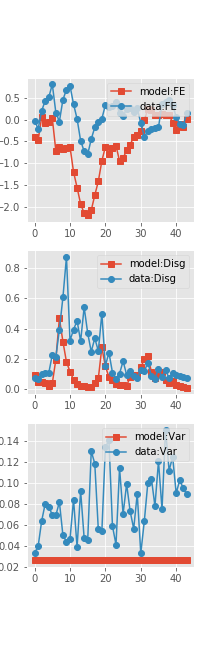
\includegraphics[width=0.19\textwidth, height = \0.95\textheight]{figures/spf_se_est_diag2.png}
		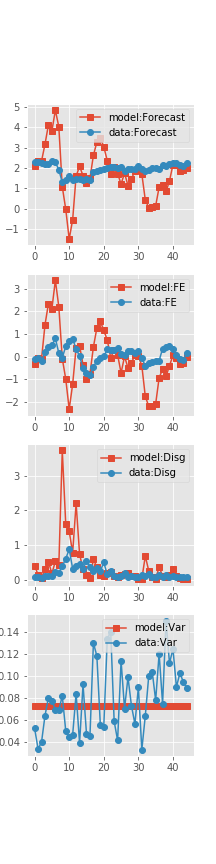
\includegraphics[width=0.19\textwidth, height = \0.95\textheight]{figures/spf_se_est_diag3.png}
		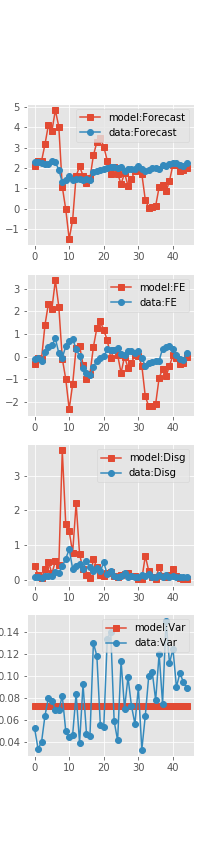
\includegraphics[width=0.19\textwidth, height = \0.95\textheight]{figures/spf_se_est_diag4.png}
\end{figure}
\end{frame}


\begin{frame}{Results: households and SEAR}
	
	\begin{frame}{Results: households and SESV}
		\begin{figure}[ht]
			\centering
			\label{SESV_diag_SCE}
			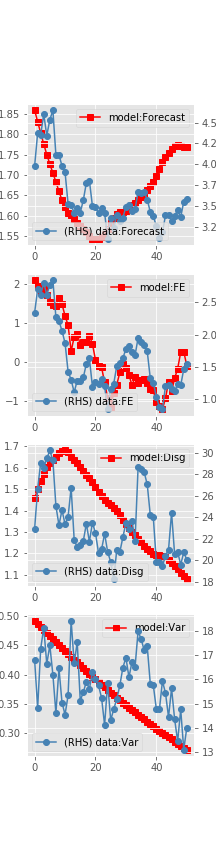
\includegraphics[width=0.19\textwidth, height = \0.95\textheight]{figures/sce_se_est_sv_diag0.png}
			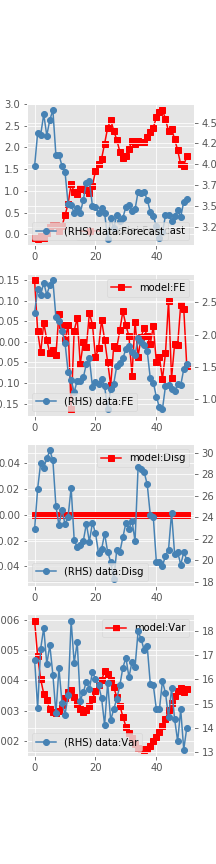
\includegraphics[width=0.19\textwidth, height = \0.95\textheight]{figures/sce_se_est_sv_diag1.png}
			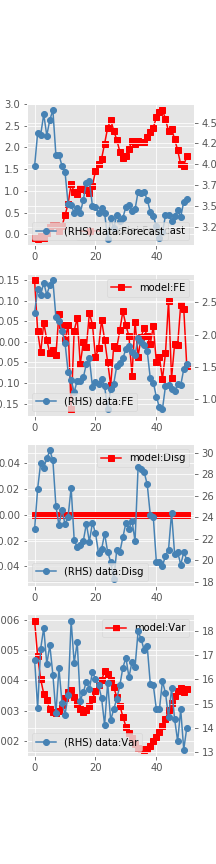
\includegraphics[width=0.19\textwidth, height = \0.95\textheight]{figures/sce_se_est_sv_diag2.png}
			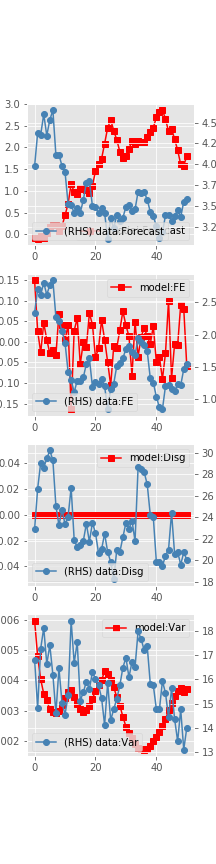
\includegraphics[width=0.19\textwidth, height = \0.95\textheight]{figures/sce_se_est_sv_diag3.png}
			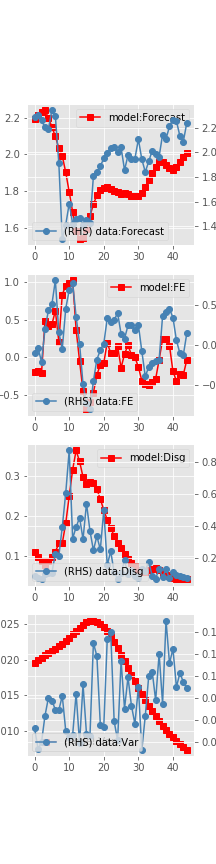
\includegraphics[width=0.19\textwidth, height = \0.95\textheight]{figures/spf_se_est_sv_diag4.png}
		\end{figure}
	\end{frame}
	
	\begin{frame}{SEAR parameters}
		\begin{figure}[ht]
			\centering
			\label{SE_diag_SCE}
			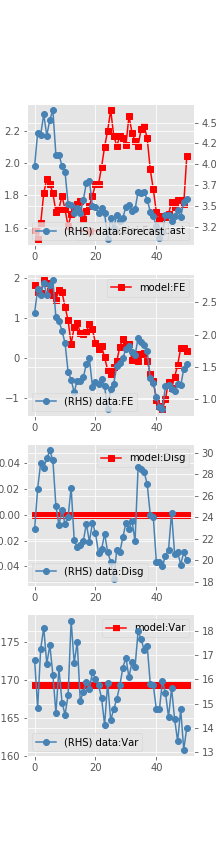
\includegraphics[width=0.19\textwidth, height = \0.95\textheight]{figures/sce_se_est_diag0.png}
			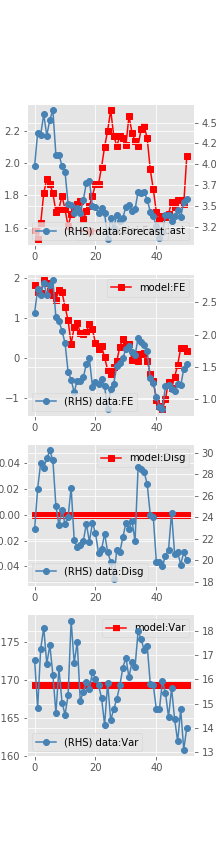
\includegraphics[width=0.19\textwidth, height = \0.95\textheight]{figures/sce_se_est_diag1.png}
			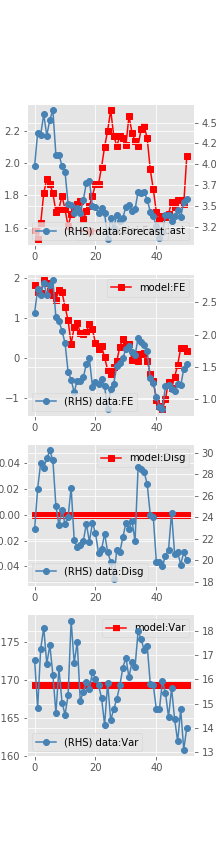
\includegraphics[width=0.19\textwidth, height = \0.95\textheight]{figures/sce_se_est_diag2.png}
			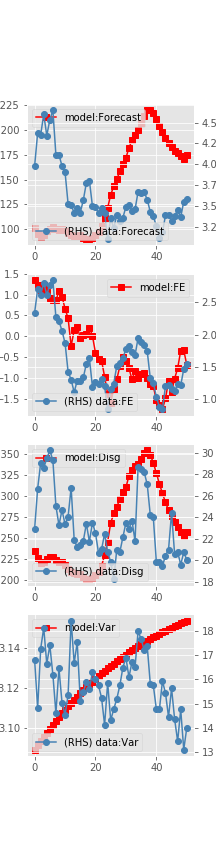
\includegraphics[width=0.19\textwidth, height = \0.95\textheight]{figures/sce_se_est_diag3.png}
			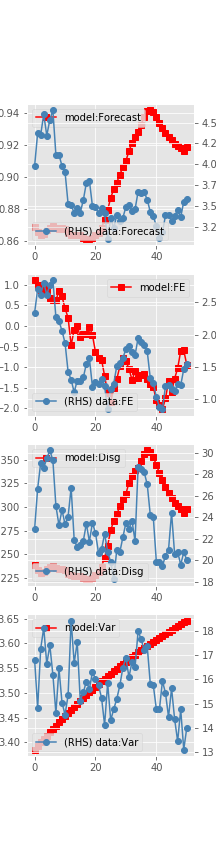
\includegraphics[width=0.19\textwidth, height = \0.95\textheight]{figures/sce_se_est_diag4.png}
		\end{figure}
	\end{frame}
	
	\begin{frame}{SESV parameters}
		\begin{table}
			\centering
			\caption{GMM Estimates of Parameters of SESV}
			\label{GMM_Est_SE_SV_Table}
			\begin{tabular}{llllll}
				\hline 
				0        & 1  & 2    & 3   & SE: $\hat\lambda_{SPF}$(Q) & SE: $\hat\lambda_{SCE}$(M) \\
				\hline 
				Forecast &    &      &     & 0.23                       & 0.01                       \\
				FE       &    &      &     & 0.12                       & 1                          \\
				Forecast & FE &      &     & 0.12                       & 1                          \\
				Forecast & FE & Disg &     & 0.12                       & 1                          \\
				Forecast & FE & Disg & Var & 0.12                       & 1           \\
				\hline               
			\end{tabular}
		\end{table}	
	\end{frame}
	
	\begin{frame}{SESV parameters}
		\begin{table}
			\centering
			\caption{GMM Estimates of Parameters of SE and Inflation Process}
			\label{GMM_Est_SE_Table}
			\begin{tabular}{llllllllllll}
				\hline 
				& 1  & 2    & 3   & SE: $\hat\lambda_{SPF}$(Q) & SE: $\hat\lambda_{SPF}$(Q) & SE: $\rho$ & SE: $\sigma$ & SE: $\hat\lambda_{SCE}$(M) & SE: $\hat\lambda_{SCE}$(M) & SE: $\rho$ & SE: $\sigma$ \\
				\hline 
				Forecast &    &      &     & 0.05                       & 0.03                       & 1          & 0.1          & 1                          & 1                          & 1          & 0.1          \\
				FE       &    &      &     & 0.05                       & 0.03                       & 1          & 0.1          & 1                          & 1                          & 1          & 0.1          \\
				Forecast & FE &      &     & 0.05                       & 0.03                       & 1          & 0.1          & 1                          & 1                          & 1          & 0.1          \\
				Forecast & FE & Disg &     & 0.7                        & 0.38                       & 0.88       & 0.1          & 0.02                       & 0.03                       & 0.98       & 0.1          \\
				Forecast & FE & Disg & Var & 0.7                        & 0.38                       & 0.88       & 0.2          & 0.01                       & 0.03                       & 0.98       & 1.11     \\
				\hline    
			\end{tabular}
		\end{table}
\end{frame}

\begin{frame}{Conclusion}
\begin{itemize}
	\item Sticky expectation(SE) matches data of inflation and expectations better compared to nosiy information (NI) 
	\item Within model,  households are more irrational compared professionals
	\item Incorporating higher moments, i.e. uncertainty helps ``discipline'' theories on expectation formation
	\item  Higher moments from surveys also contain useful information about the inflation dynamics itself
\end{itemize}	
\end{frame}


\bibliographystyle{apalike}
\bibliography{ExpSlides}

\section{Appendix}

\end{document}
